% !TeX encoding = UTF-8
% !TeX program = pdflatex
% !TeX spellcheck = en-UK
%Qui tutto ciò che c’ è da saper su LaTeX: http://www.lorenzopantieri.net/LaTeX_files/ArteLaTeX.pdf
%Per scrivere la bibliografia puoi vedere il seguente link: https://www.guitex.org/home/images/doc/GuideGuIT/bibliografia.pdf
% Per usare in locale questo progetto latex è necessario eseguire le seguenti installazioni:
% sudo apt install texlive texstudio texlive-publishers texlive-latex-extra texlive-fonts-extra texlive-science texlive-bibtex-extra texlive-lang-english

\documentclass[a4paper, oneside]{sapthesis}

%pacchetti per LaTeX
\usepackage[english]{babel}
\usepackage[utf8]{inputenc}
\usepackage{imakeidx}
\usepackage[acronym]{glossaries}
\usepackage{appendix}
\usepackage[colorlinks=true]{hyperref}
\usepackage{cleveref}
\usepackage{enumitem}
\usepackage{marginnote}
\usepackage{tocloft}
\usepackage{float}
%pacchetti matematici
\usepackage{amssymb}
\usepackage{mathtools}
\usepackage{amsmath}
\usepackage{amsthm}
\usepackage{siunitx}
% ATTENZIONE: c'è un bug in thmtools, per approfondire vedere: https://tex.stackexchange.com/questions/305174/proof-environment-produces-proof-proof-only-when-thmbox-is-used
\usepackage{letltxmacro}
\LetLtxMacro\amsproof\proof
\LetLtxMacro\amsendproof\endproof
\usepackage{thmtools}
\AtBeginDocument{%
	\LetLtxMacro\proof\amsproof
	\LetLtxMacro\endproof\amsendproof
}
\usepackage{dsfont}
%pacchetti per le immagini
\usepackage{graphicx}
\usepackage{subcaption}
\usepackage{color}
\usepackage[dvipsnames, table]{xcolor}
%pacchetti per la scrittura di codice
\usepackage{listings}
\usepackage{algorithm}
\usepackage{algpseudocode}
\usepackage{algorithmicx}
%pacchetti per la gestione di citazioni e bibliografia
\usepackage[sort]{natbib}
\usepackage{comment}


\bibliographystyle{plainnat} %ordine della bibliogragia
\setcitestyle{numbers}
\setcitestyle{square}

%preparazione SAPthesis
\title{Exploring Authorial Identity through Data Mining Techniques}
\subtitle{Analyzing Artistic Traits for Authorship Attribution}
\author{Stefano Magrini Alunno}
\IDnumber{1851728}
\course{Master degree in Applied Mathematics}
\courseorganizer{Faculty of Mathematics, Physics and Natural Sciences}
\AcademicYear{2023/2024}
\advisor{Prof. Grabriella Anna Puppo}
%\customadvisorlabel{Advisor}
\authoremail{stefanomagrini99@gmail.com}
\copyyear{2024}
\thesistype{Master thesis}
\examdate{00/00/00}
\examiner{Prof. uno}  % presidente
\examiner{Prof. due}
\examiner{Prof. tre}
\examiner{Prof. ...}
\examiner{Prof. ...}
\examiner{Prof. ...}
\examiner{Prof. ...}
\versiondate{\today}

%preparazione
\lstdefinestyle{code}{
    backgroundcolor=\color{white},
    commentstyle=\bfseries\itshape\color{gray},
    basicstyle=\ttfamily\scriptsize,
    keywordstyle=\color{blue},
    numberstyle=\tiny\color{gray},
    numbersep=5pt,
    stringstyle=\color{orange},
    showspaces=false,
    showstringspaces=false,
    showtabs=true,
    numbers=left,
    prebreak=\raisebox{0ex}[0ex][0ex]{\ensuremath{\hookleftarrow}},
    captionpos=t,
    frame=bottomline,
    breakatwhitespace=true,
    breaklines=true,
    keepspaces=true,
    tabsize=2,
    escapeinside={\%*}{*)}
}
\definecolor{Teal}{rgb}{0.0, 0.5, 0.5}
\hypersetup{
	colorlinks=true,
	linkcolor=MidnightBlue,
	citecolor=ForestGreen,
	filecolor=RoyalPurple,
	urlcolor=Teal,
	pdftitle={Exploring Authorial Identity through Data Mining Techniques},
	pdfauthor={Stefano Magrini Alunno},
	pdfkeywords={Latex, hyperref, hyperlink}
}

\definecolor{revisioncolor}{RGB}{25, 25, 112}
\definecolor{modifiedcolor}{RGB}{128, 0, 32}
\definecolor{todocolor}{RGB}{34, 139, 34}
\definecolor{notecolor}{RGB}{102, 68, 34}
\newenvironment{toReview}{\addtoReview\color{revisioncolor}\marginnote{\textbf{To Review}}}{\ignorespacesafterend}
\newenvironment{modified}{\addmodified\color{modifiedcolor}\marginnote{\textbf{Modified}}}{\ignorespacesafterend}
\newenvironment{toDo}{\addtoDo\color{todocolor}\marginnote{\textbf{To Do}}}{\ignorespacesafterend}
\newenvironment{note}{\addnote\color{notecolor}\marginnote{\textbf{Note}}}{\ignorespacesafterend}
\newlistof{ambienti}{amb}{Special contents}
\newcommand{\customindex}{\listofambienti}
\newcommand{\addtoReview}{\addcontentsline{amb}{ambienti}{To Review}}
\newcommand{\addmodified}{\addcontentsline{amb}{ambienti}{Modified}}
\newcommand{\addtoDo}{\addcontentsline{amb}{ambienti}{To Do}}
\newcommand{\addnote}{\addcontentsline{amb}{ambienti}{Note}}

\definecolor{kernel}{rgb}{0.96,0.9,0.9} % 0.9 luminosità, 0.6 saturazione, (1,0,0)
\definecolor{python}{rgb}{0.9,0.96,0.9} % 0.9 luminosità, 0.6 saturazione, (0,1,0)
\definecolor{source}{rgb}{0.9,0.9,0.96} % 0.9 luminosità, 0.6 saturazione, (0,0,1)
\lstdefinestyle{CCode}{
	backgroundcolor = \color{source},
	breakatwhitespace=false,
	breaklines=true,
	captionpos=b,
	commentstyle=\color{ForestGreen},
	firstnumber=1,
	keepspaces=true,
	keywordstyle=\bfseries\color{blue},
	language=C,
	morekeywords={*,...},
	numbers=left,
	numbersep=5pt,
	numberstyle=\tiny\color{gray},
	showspaces=false,
	showstringspaces=false,
	stringstyle=\itshape\color{orange},
	tabsize=2
}
\lstdefinestyle{CuCode}{
	backgroundcolor = \color{kernel},
	breakatwhitespace=false,
	breaklines=true,
	captionpos=b,
	commentstyle=\color{ForestGreen},
	firstnumber=1,
	keepspaces=true,
	keywordstyle=\bfseries\color{blue},
	language=C,
	morekeywords={*,...},
	numbers=left,
	numbersep=5pt,
	numberstyle=\tiny\color{gray},
	showspaces=false,
	showstringspaces=false,
	stringstyle=\itshape\color{orange},
	tabsize=2
}
\lstdefinestyle{PyCode}{
	backgroundcolor = \color{python},
	breakatwhitespace=false,
	breaklines=true,
	captionpos=b,
	commentstyle=\color{ForestGreen},
	firstnumber=1,
	keepspaces=false,
	keywordstyle=\bfseries\color{blue},
	language=Python,
	morekeywords={*,...},
	numbers=left,
	numbersep=5pt,
	numberstyle=\tiny\color{gray},
	showspaces=false,
	showstringspaces=false,
	showtabs=false,
	stringstyle=\itshape\color{orange},
	tabsize=2
}

% 3 famiglie: remark, definition, theorem
% remark: la massima utilità è aiutare la comprensione, contiene:
    % remark
    % exempli gratia
\declaretheorem[
    name=Remark,
    numbered=no,
    style=remark
]{remark}
\declaretheorem[
    name=Exempli Gratia,
    numbered=no, shaded,
    style=remark
]{exempli_gratia}
\declaretheorem[
    name=Definition,
    numberwithin=section, shaded,
    style=definition
]{definition}
\declaretheorem[
    name=Notation,
    numbered=no, shaded,
    style=definition
]{notation}
\declaretheorem[
    name=Theorem,
    numberwithin=chapter, thmbox=M,
    style=plain
]{theorem}
\declaretheorem[
    name=Proposition,
    numberwithin=section,
    style=plain
]{proposition}
\declaretheorem[
    name=Lemma,
    numberwithin=section,
    style=plain
]{lemma}
\declaretheorem[
    name=Corollary,
    numbered=no,
    style=plain
]{corollary}

\algnewcommand{\Where}[2]{\State \textbf{where}\ #1\ \textbf{do} #2}

\definecolor{mint}{rgb}{0.68, 0.92, 0.70}
\definecolor{lavender}{rgb}{0.93, 0.57, 1.0}
\definecolor{ambra}{rgb}{1.0, 0.75, 0.0}

\includeonly{
    abstract,
    acknowledgments,
    glossary,
    bibliography,
    main/Introduction,
    main/LiteratureReview,
    main/Methodology,
    main/Discussion,
    main/Conclusion,
    main/Results,
    main/Appendix
}

\makeindex
\makeglossaries  % produce il glossario
\newglossaryentry{boost}
{
    name=boost,
    description={In computer science, "boost" generally refers to enhancing the performance of a system, application, or algorithm through code optimization, leveraging more efficient hardware resources, or implementing advanced techniques}
}
\newglossaryentry{thread}
{
    name=thread,
    description={A thread is a fundamental unit of execution in computing, allowing a program to perform multiple tasks concurrently, akin to different lines of thought in a mathematical problem-solving process}
}
\newglossaryentry{warp}
{
    name=warp,
    description={A warp is a group of threads executed together in a synchronized manner within a GPU, allowing for efficient parallel processing of data}
}
\newglossaryentry{kernel}
{
    name=kernel,
    description={A kernel in GPU programming refers to a small program or function that is executed in parallel across multiple threads on a GPU, typically used to perform computations on large datasets or to accelerate specific tasks}
}
\newglossaryentry{Python}
{
    name=Python,
    description={A high-level, general-purpose programming language}
}
\newglossaryentry{CUDA}
{
    name=CUDA,
    description={Dialect of the C++ language for handling the video card}
}
\newglossaryentry{VSCode}
{
name=VSCode,
description={Popular free, open-source code editor that integrates with GitHub for version control and supports Python debugging}
}
\newglossaryentry{dataset}
{
    name=dataset,
    description={A data set is a collection of data}
}
\newglossaryentry{png}
{
    name=png,
    description={The PNG (Portable Network Graphics) format is a raster image file format used for lossless compression. This means that images saved in this format do not lose quality or detail during compression}
}
\newglossaryentry{kmeans}
{
    name=KMeans,
    description={K-means is an unsupervised clustering algorithm that divides a data set into k distinct groups based on distance. Each group is defined by its centroid, and the goal of the algorithm is to minimise the variance within the groups}
}
\newglossaryentry{cxx}
{
    name=C++,
    description={A general-purpose computer language widely used to build high-performance code for embedded systems}
}
\newglossaryentry{gdb}
{
name=gdb,
description={GDB is a debugger for C, C++, and CUDA code, allowing step-by-step execution and inspection of programs to identify and fix issues}
}
\newglossaryentry{thrust}
{
    name=thrust,
    description={libreria di C++ che può gestire anche dati attraverso il processore grafico}
}
\newglossaryentry{cuBLAS}
{
    name=cuBLAS,
    description={libreria di CUDA-Toolkit specializzata nel calcolo lineare e gestione di dati su processori grafici}
}
\newglossaryentry{cursedim}
{
name=curse of dimensionality,
description={The curse of dimensionality refers to various phenomena that arise when analyzing and organizing data in high-dimensional spaces that do not occur in low-dimensional settings}
}
\newglossaryentry{montecarlo}
{
	name=Monte Carlo method,
	description={Monte Carlo methods, or Monte Carlo experiments, are a broad class of computational algorithms that rely on repeated random sampling to obtain numerical results}
}
\newglossaryentry{r}
{
name=R,
description={A computer language used mostly for statistical analysis. Includes not only many features but also datasets}
}
\newglossaryentry{Linux}
{
name=Linux,
description={Linux is an open-source operating system known for its stability, security, and flexibility, widely used in servers and development environments}
}
\newglossaryentry{doxygen}
{
name=Doxygen,
description={Doxygen is a documentation generator for C, C++, and other programming languages, used to create software documentation from source code comments}
}
\newglossaryentry{sphinx}
{
name=sphinx,
description={Sphinx is a documentation generator for Python, commonly used to create intelligent and readable project documentation in formats like HTML and PDF}
}
\newglossaryentry{github}
{
name=GitHub,
description={GitHub is a platform for version control and collaboration, allowing developers to host, share, and manage code using Git}
}

% sigle che fanno riferimento al progetto stesso
\newacronym{dada}{DADA}{Discrete Automatic Drawings' Analysis}
\newacronym{cada}{CADA}{Continuous Automatic Drawings' Analysis}

% sigle per termini informatici
\newacronym{gpu}{GPU}{Graphics Processing Unit}
\newacronym{cpu}{CPU}{Central Processing Unit}
\newacronym{rgb}{RGB}{Red Green Blue}
\newacronym{hsl}{HSL}{Hue Saturation Lightness}
\newacronym{gpgpu}{GPGPU}{General-Purpose computing on Graphics Processing Units}
\newacronym{sm}{SM}{Stream Multi-Processing}
\newacronym{hpc}{HPC}{High Performance Computing}
\newacronym{cuda}{CUDA}{Compute Unified Device Architecture}

% sigle per termini tecnici generici
\newacronym{dpi}{DPI}{dots per inch}

% sigle matematiche
\newacronym{gmm}{GMM}{Gaussian Mixture Models}
\newacronym{svd}{SVD}{Singular Value Decomposition}
\newacronym{fft}{FFT}{Fast Fourier Transform}
\newacronym{dft}{DFT}{Discrete Fourier Transform}
\newacronym{cft}{CFT}{Continue Fourier Transform}
\newacronym{idft}{IDFT}{Inverse Discrete Fourier Transform}

% sigle per termini teorici
\newacronym{fcm}{FCM}{Fuzzy C-Means Clustering}
\newacronym{em}{EM}{Expectation-Maximisation}
\newacronym{map}{MAP}{Maximum A Posteriori}


\begin{document}

\frontmatter
\maketitle
\dedication{Mater artium necessitas}
%\begin{abstract}
The attribution of authorship in graphic works is a topic of interest in various fields, including art history, intellectual property protection and digital forensics. This thesis represents a continuation of my previous thesis (\cite{thesis}), which proposed a pioneering method for authorship attribution based on a simplified representation of images. The aim was to address some of the more obvious limitations of the previous methodology, such as the inflexibility of pre-processing and the need to work with binary images.

\noindent In this paper, a new application based on fuzzy clustering techniques (FCM) is introduced. This application enables the analysis of greyscale images, improving the model's ability to adapt to complex and noisy data. Although the method still has significant limitations in terms of reliability compared to more established techniques, it represents a first step towards an idea that, if developed further, could offer an interesting alternative.

\noindent The methodology was applied to a dataset of $113$ sheets of university notebooks, with results showing a false negative rate of $6\%$ and a false positive rate of $18\%$. Although these results are not perfect, they highlight the potential of the proposed method and suggest directions for future investigation.

\noindent It is important to note that the intention of this paper is not to replace traditional methods, but rather to propose a complementary avenue that, with further development, could enhance the existing range of authorial attribution techniques.
\end{abstract}

\tableofcontents
\newpage
\listoffigures
\newpage
\listoftables
\newpage
\customindex
\printglossary[type=\acronymtype]
\phantomsection
\addcontentsline{toc}{chapter}{Acronyms}

\mainmatter
%\chapter{Introduction}
%Introduco la tesi magistrale.
\begin{toReview}
	\section{Attribution of handwriting works}
		\noindent The comparison of graphic works plays a very important role in several fields, including art history, digital forensics and intellectual property protection. By analysing the characteristics of graphic works, it is possible to identify the author, verify the authenticity of a work or detect possible counterfeits. In art history, for example, stylistic and technical analysis of handwritten notes or sketches can provide valuable insights into the creative processes of renowned authors. Similarly, in digital forensics, the comparison of graphic works can help detect counterfeit documents or identify alterations to legal documents.

		\noindent Beyond these practical applications, the ability to compare graphic works also opens up possibilities for understanding more general patterns. For example, it can help uncover stylistic influences between artists or identify recurring patterns within a collection. In the context of machine learning and data analysis, graphical comparison serves as a basis for developing algorithms capable of processing complex visual data, which is increasingly important in an era dominated by digital media.

		\noindent However, the process is not without its challenges. The presence of noise, variations in resolution and the diversity of graphical styles make it difficult to establish a robust and reliable framework for comparison. This thesis aims to address these issues by developing methods to improve the accuracy and adaptability of graphical work comparisons.

		\bigskip
		\noindent The practical applications of comparing graphic works cover a wide range of fields, each of which benefits from customised analysis techniques:

		\begin{itemize}
			\item \textbf{Authorship attribution}: Determining the author of a handwritten document or artistic work is important in fields such as art history, where verifying the authenticity of an artist can have a significant impact on the cultural and financial value of the work.
			\item \textbf{Falsification Detection}: In digital forensics and legal investigations, identifying alterations to documents or detecting forgeries in graphic works plays a key role in ensuring authenticity and legality.
			\item \textbf{Intellectual Property Protection}: The ability to compare graphic works is critical for enforcing copyright laws and resolving disputes over original creations.
			\item \textbf{Historical Analysis}: In the study of historical documents and manuscripts, graphic comparison helps to trace stylistic influences, identify authors, and reconstruct fragmented works.
			\item \textbf{Digital Archiving and Restoration}: Automated comparison methods help to cluster, catalogue and restore large collections of graphic works, ensuring their preservation for future generations.
		\end{itemize}

		\noindent These applications demonstrate the versatility and importance of robust graphical comparison methods. Each context presents unique challenges, such as the need to handle different resolutions, styles and noise levels, which this thesis aims to address through innovative methods.

		\bigskip
		\noindent Despite its importance, the comparison of graphic works faces several challenges and limitations that have hindered progress in the field:

		\begin{itemize}
			\item \textbf{Distortions and impurities}: Graphic works, especially handwritten or historical documents, often contain noise such as background patterns, stains or scanning distortions. These contaminants can distort the analysis and reduce the reliability of the comparison results.
			\item \textbf{Variability in resolutions and formats}: Works are often digitised at different resolutions and stored in different formats, making it difficult to standardise data for analysis. This variability makes it difficult to extract meaningful features.
			\item \textbf{High dimensionality and computational cost}: Graphic works are represented as high-dimensional data, especially when detailed features or pixel-level analysis are involved. This increases computational costs and limits the feasibility of large-scale comparisons.
			\item \textbf{Limited robustness of clustering techniques}: Traditional clustering methods, such as hard \gls{kmeans}, struggle with noisy and overlapping data distributions, leading to suboptimal results in many real-world scenarios.
			\item \textbf{Lack of standardised datasets}: The lack of well-curated and representative datasets for testing and validating comparative methods makes it difficult to benchmark algorithms and ensure their generalisability.
			\item \textbf{Subjective pre-Processing Steps}: Many pre-processing techniques depend on manual adjustments or heuristics, which can introduce bias and limit the reproducibility of the analysis.
		\end{itemize}

		\noindent These issues highlight the need for advanced methods that can adapt to noise, handle different data representations, and provide reliable results in a range of scenarios. This thesis directly addresses these challenges by refining preprocessing techniques, introducing fuzzy clustering for improved robustness, and exploring scalable solutions for high-dimensional data.

	\section{Background of the project}
		In my thesis \cite{thesis}, an attempt was made to adapt an authorship attribution method similar to that proposed in \cite{SapAttribution}, which uses the $n$-gram model advanced by \citet{Shannon_ngrammodel}. This method has several distinctive features:
		\begin{itemize}
			\item The $n$-gram model was originally designed to emulate natural language rather than images.
			\item Applying this idea to attributing authorship to images introduces a high degree of complexity, especially in preventing falsifications.
		\end{itemize}

		\noindent Another remarkable aspect of the attribution process is the comparison formula defined in \cite{SapAttribution} and later adopted in \cite{thesis}. This formula defines a comparison function between discrete distributions: the unknown work is compared to all known works, and the results of this function are analysed to determine the most likely author.

		\noindent However, the nature of this comparison formula, as presented in \cite{thesis}, was not well suited to graphic works. This necessitated a pre-processing phase in which images were converted into matrices of black and white pixels, which simplified the representation of the data but introduced limitations in the handling of more complex graphical features.

		\bigskip \noindent One of the main problems encountered in \cite{thesis} is the significant loss of information caused by the pre-processing phase. A graphic work had to be processed by eliminating shades or editing entire noisy regions. The comparison formula, by its very nature, emphasises details and the presence of high noise is a serious obstacle. For this reason, in \cite{thesis}, we chose to work with manuscripts produced on a tablet, thus ensuring a controlled environment free of impurities. The results were remarkable: almost all the works analysed were correctly attributed.

		\noindent However, it was observed that this methodology has significant limitations when applied to works of a different nature. The success of the experiment is largely attributable to the fact that writing, by its very nature, is an image composed of small regions that are either very light or very dark. This drastically reduced the negative effects of pre-processing, such as the destruction or creation of information. With less controlled data, such as images from real sheets instead of a tablet, numerous problems could have been caused, compromising the effectiveness of the method.

		\bigskip \noindent In this thesis, we investigate the possibility of creating a variant for colour images, thus eliminating the main problem identified in \cite{thesis}: pre-processing. The aim is to develop a new theory that, unlike in \cite{thesis} and \cite{SapAttribution}, does not require the discretization of the data. This is a significant step in terms of application, as a colourful image is expected to provide a higher level of matching accuracy.

		\noindent However, this idea presents some fundamental challenges. The formula for comparing works, as defined in \cite{SapAttribution}, is not directly compatible with colourful images, and the inherent continuous nature of colours may cause the model to consider the works all equally distinct. In addition, the $n$-gram model of \citeauthor{Shannon_ngrammodel} is well suited to natural language words, but less effective for images, which are more susceptible to noise and require an appropriate metric to interpret them.

		\bigskip \noindent To realise the idea of attributing works without pre-processing, several methodologies were explored:

		\begin{enumerate}
			\item \textbf{Represent the work as a surface in colour space}: Although interesting, this proposal presented significant difficulties in defining an effective way of comparing two works.
			\item \textbf{Using the Wasserstein distance to compare distributions}: This method proved to be extremely computationally expensive and inefficient, as it did not give sufficient weight to the details of the work, an important element in attribution.
			\item \textbf{Discretising the union of distributions by clustering}: This approach finally showed the greatest potential and formed the basis for the development of this thesis.
		\end{enumerate}

		\noindent The central question around which this thesis revolves is: is it possible to attribute graphical works using a dynamic discretisation of space? In other words, the comparison function defined in \cite{SapAttribution} is seen as an approximate integral over boxes. In fact, by using a matrix with black and white pixels, we have divided the space into boxes of equal size. This method, already used in \cite{thesis}, allows an efficient approximation when the number of boxes is not too large compared to the sparsity of the $n$-grams.

		\noindent In this thesis, an alternative is proposed: replacing boxes with clustering algorithms. These algorithms successfully handle high-dimensional sparsity problems by offering a more adaptive discretisation that serves as the basis for redefining the comparison formula.

		\bigskip \noindent This thesis introduced significant changes not only in the comparison methodology, but also in the pre-processing phase. It was no longer acceptable to work with a ‘perfect’ dataset; it was necessary to use a real, and therefore inevitably ‘dirty’ dataset. After much difficulty, it was possible to collect a dataset of $113$ university note sheets. However, the quality of the images was insufficient for an accurate analysis, making pre-processing indispensable, which, although minimal, could still have compromised the project. This pre-processing phase was limited to image cleaning and greyscale conversion, an operation that, for university notes, should not have a significant impact.

		\noindent Another major change affected the image synthesis phase. In \cite{thesis}, images were transformed into a list of $n$-grams with their respective occurrence in the work. However, as this aspect was no longer central to the proposed methodology, it was preferred to simply provide a list of the extracted tiles.

	\section{Key points}
		As already pointed out, the collection of the dataset presented considerable difficulties, making manual collection necessary. For this research, dozens of university notebooks were made available, from which $113$ pages were selected and scanned. The final result comprises $420$ uncompressed image fragments, totalling $1.1\operatorname{\mathrm{Gb}}$, with a resolution of $400$ \gls{ppi}. The dataset includes one main author (\texttt{Author 1}), representing more than half of the works, and three other secondary authors whose purpose is to complicate attribution.

		\noindent The lack of a professional dataset and the very nature of the notebooks required careful pre-processing. Indeed, university notebooks have a background with a grid of squares that can confuse the algorithm, leading it to mistake this structure for human handwriting. Removing the squares without compromising the handwriting details was one of the main challenges faced.

		\noindent Once a method for comparing the works had been defined, it was necessary to implement the algorithms required for the calculations. As no frameworks were available to directly support the more computationally onerous operations on \gls{gpu}, a customised solution was opted for using \gls{Python} and \gls{cuda}, producing tools capable of handling both high and low-level data and calculations.

		\noindent In-depth analyses were conducted to produce accurate results, taking into account the physical and temporal limitations of computational resources. Each step was carefully examined, testing various techniques and parameters to optimise the process.

		\noindent This thesis introduces clustering \gls{fcm} as a generalisation of the work carried out in \cite{thesis}, demonstrating its effective implementation and application, and laying the groundwork for further developments in the automatic comparison of graphical works.

		\bigskip \noindent In summary, in \cite{thesis}, image analysis consists of three main steps:

		\begin{itemize}
			\item \textbf{Pre-processing}: Images are transformed into matrices of black and white pixels.
			\item \textbf{Synthesis}: The pixel matrices are converted into a list of tiles with their respective occurrences.
			\item \textbf{Comparison}: The formula defined in \cite{SapAttribution} is used to compare works.
		\end{itemize}

		\noindent In this thesis, the three phases have been redefined as follows:

		\begin{itemize}
			\item \textbf{Pre-processing}: The images are converted to greyscale with a specific resolution (\gls{ppi}) and then cleaned of pollutants by cutting and removing squares.
			\item \textbf{Synthesis}: An ordered list of tiles with their respective occurrences is no longer generated, but only an unordered list of tiles with repetitions.
			\item \textbf{Comparison}: A new comparison formula is developed that dynamically discretizes the space of tiles by clustering.
		\end{itemize}

		\noindent This paper illustrates the main sources in the Literature Review section, providing the intuitive basis for applying them to the context at hand. The $n$-gram model of \citet{Shannon_ngrammodel} and its use in \cite{SapAttribution} and \cite{thesis} will be introduced. Furthermore, clustering concepts and related algorithms, including \gls{kmeans}, \gls{fcm} and \gls{gmm}, will be discussed and compared. Finally, the algorithm \gls{fft} for removing squares in images will be presented.

		\noindent After having introduced the fundamental concepts, these will be explored in detail from both an implementation and theoretical point of view in the Methodology chapter. Here, the new comparison formula will be shown and design choices will be evaluated by means of synthetic examples.

		\noindent Once the code has been developed and the theoretical foundations clarified, the direct application on the dataset will be described in the chapter Results, where the parameters will be refined and detailed qualitative results given.


\end{toReview}
  % Introduzione
\chapter{Literature Review}
\label{chap:LiteratureReview}
This chapter reviews key literature that forms the theoretical foundation of this research. Specifically, the $n$-gram language model, fuzzy clustering, and Fourier transforms will be discussed. Additionally, specific details of these topics will be examined to demonstrate their practical applications within this project.

\noindent Relevant definitions and properties needed to understand these applications will be introduced, alongside examples and comparisons to provide a more comprehensive and nuanced understanding of the theory.

\section{n-gram language model}
The $n$-gram language model analyzes a sequence of symbols by examining sets of frames, known as $n$-grams. This model is designed to construct a natural language model based on the assumption that each new symbol is statistically influenced by the preceding symbols. For example, the phrase '\texttt{I am playing }' could be followed by '\texttt{a piano}' or '\texttt{with a dog}'. The $n$-gram model assumes that the continuation of this phrase depends solely on a finite window of preceding words or characters, and assigns '\texttt{a piano}' a certain probability of being the most natural continuation. However, as language modeling techniques have advanced, the $n$-gram model has largely been replaced by more sophisticated models, such as transformers\footnote{For more information on transformers, see \url{https://en.wikipedia.org/wiki/Transformer_(deep_learning_architecture)}}.

\begin{figure}[ht]
	\centering
	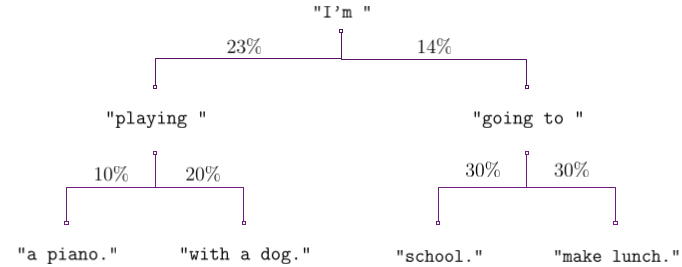
\includegraphics[width=\linewidth]{Figures/exngrammodel.png}
\end{figure}

\noindent The $n$-gram language model, first introduced by Shannon and described in \citet{Shannon_ngrammodel}, was later applied in \citet{SapAttribution} for the purpose of author attribution. In this case, the goal was not to generate natural text but to identify the author of a given text. The research found that the best performance was achieved using $8$-grams, and attribution was done by comparing each known author's work with the target text.

\noindent An additional development of this model extended its use to a completely different field: images. In the research thesis \cite{thesis}, this attribution method was employed to determine the authorship of a manuscript by treating the grams as square pixel tiles.

\subsection{Insights}
As previously mentioned, the $n$-gram model predicts the next characters or words to be placed based on the preceding ones. For example, if the focus is on sequences of $n$ printable characters, the model is trained on a dataset of text files, empirically deriving the probabilities $\mathbb{P}\left[w_n|w_1,\dots,w_{n-1}\right]$, where $w_i$ represents the $i$-th character of the $n$-gram.

\begin{toReview}
	\noindent In this way, a machine can construct a sentence from a few characters: $w_1,\ldots,w_{n-1}$. The algorithm iteratively selects the most probable next character $w_{n}$ given the current window of $n-1$ characters, then updates the window to $w_2,\ldots,w_{n}$ to predict $w_{n+1}$, and so on. This step-by-step process resembles a Markov chain, where each state corresponds to the current sequence of characters, and transitions between states occur with probabilities derived from the dataset.
\end{toReview}

\begin{modified}
\noindent The model assumes that the next character  depends only by the last $n-1$ characters so:
\begin{equation}
	\mathbb{P}\left[w_{n+k}|w_k\dots w_{n+k-1}\right] = \mathbb{P}\left[w_{n+k}|w_{k+1}\dots w_{n+k-1}\right] \quad \forall k
	\label{eq:ngram_model}
\end{equation}
\end{modified}
From this assumption we derive the following property:
\begin{proposition}
	\begin{modified}
		Let $w_1,\dots,w_{n-1},w_n\dots,w_{n+k}$ be a sequence of characters, where $n$ represents the size of the $n$-gram window used by the model. Specifically, the model assumes that the probability of the $n$-th character depends only on the preceding $n-1$ characters for all $n$-grams. We have that:
	\end{modified}
\begin{equation}
	\mathbb{P}\left[w_n,\dots,w_{n+k}|w_1,\dots,w_{n-1}\right] = \prod_{i=0}^{k}\mathbb{P}\left[w_{n+i}|w_{i+1}\dots w_{n+i-1}\right]
	\label{eq:ngram_model_prop}
\end{equation}
\end{proposition}

\begin{proof}
	This property is proved by using Bayes' theorem and the assumption of the model \cref{eq:ngram_model}:
\begin{align*}
	\mathbb{P}\left[w_n,\dots,w_{n+k}|w_1,\dots,w_{n-1}\right] &= \prod_{i=0}^{k}\mathbb{P}\left[w_{n+i}|w_1\dots w_{n+i-1}\right] \\
	&= \prod_{i=0}^{k}\mathbb{P}\left[w_{n+i}|w_{i+1}\dots w_{n+i-1}\right]
\end{align*}
\end{proof}

\noindent The model is built on the assumption that considering $n$-grams larger than $n$ is unnecessary. However, this limitation can introduce significant weaknesses in natural language processing, as it ignores information outside the $n$-character window. For instance, in a mystery novel, understanding the entire plot and its intricate details is crucial, something the model might overlook. Despite this, the $n$-gram model can still be quite effective in simpler contexts like everyday conversation. For example, after the input '\texttt{Hi! How are }', the model might predict '\texttt{you?}' as a natural continuation.

\noindent As mentioned earlier, this model was repurposed for a different goal by \citet{SapAttribution}. While the $n$-gram model might struggle to generate fully coherent natural language without encountering semantic inconsistencies or syntactic errors, it remains useful for capturing an author's writing style. This is achieved by training the model exclusively on texts by that author. The approach is to extract all $n$-grams from the target work and compare their distribution to that of known works by other authors. The proposed formula for comparing work $A$ with work $B$ is as follows:
\begin{equation}
	d(A,B) = \frac{1}{|D_A|+|D_B|}\sum_x\left(\frac{f_A(x)-f_B(x)}{f_A(x)+f_B(x)}\right)^2
	\label{eq:SapAttribution_dist}
\end{equation}
where $f_A(x)$ represents the frequency of the $n$-gram $x$ in the work $A$ and $|D_A|$ is the variety of observed $n$-grams.

\noindent As highlighted in \cite{thesis}, two relevant properties of this method of comparing distributions can be mentioned:
\begin{itemize}
	\item Each addendum of the summation takes on a value between $0$ and $1$.
	\item The external factor not only normalises the result so that it remains between $0$ and $1$, but also calls up the Jaccard index\footnote{For more about Jaccard index, see \url{https://en.wikipedia.org/wiki/Jaccard_index}}, improving the arithmetic mean of the summation:
	\[
		\frac{1}{|D_A|+|D_B|} = (1+J_{D_A,D_B})^{-1}\frac{1}{|D_A\cup D_B|}
	\]
	\begin{toReview}
		\noindent where $J_{D_A,D_B} := \frac{\left|D_A\cap D_B\right|}{\left|D_A\cup D_B\right|}$.

		\noindent In this way, we can see the comparison formula as a product between two types of index:
		\[
			d(A,B)=(1+J_{D_A, D_B})^{-1} \times \frac{1}{\left|D_A\cup D_B\right|}\sum_{x\in D_A\cup D_B}\left(\frac{f_A(x)-f_B(x)}{f_A(x)+f_B(x)}\right)^2
		\]
	\end{toReview}
\end{itemize}

\subsection{Implications}
We conclude this section by discussing the implications of this theory. As seen in \cref{eq:ngram_model}, no distinction is made between one $n$-gram and another. This is because $n$-grams of length 3, or slightly longer, are typically used, which are insufficient to cover a full word. However, when using $7$-grams, it becomes possible to consider the relationships between synonyms and distances between $n$-grams. For instance, we would expect some level of correlation between ‘\texttt{paper}’ and ‘\texttt{article}’ as they are synonyms.

\noindent In written texts, this rarely impacts the outcome, as there are relatively few synonyms for each term within the full vocabulary, and especially few long chains of synonyms. For example, it is unlikely that many synonyms for ‘\texttt{paper}’ begin with the string ‘\texttt{p}’ or ‘\texttt{pe}’.

\noindent As noted in \cite{thesis}, the research deliberately set appropriate image \textit{resolution} and \textit{posterization} to avoid discussions about the similarity between tiles. By controlling these parameters, the focus remained on the attribution process rather than getting lost in complex considerations of tile ‘synonyms’ and their potential concatenations.

\bigskip
We further examine the properties of the comparison formula defined in  \cref{eq:SapAttribution_dist}, particularly focusing on the problem of sparsity in $n$-grams.

\noindent Let $N$ represent the samples drawn from two absolutely continuous distributions $\mathcal{A}$ and $\mathcal{B}$ defined on $\mathbb{R}$. We partition $\mathbb{R}$ into intervals (boxes) of amplitude $1 \; / \; C$, thus transforming the original distributions into their discretized versions, $\mathcal{A}(C)$ and $\mathcal{B}(C)$, along with their respective samples.

\begin{figure}[ht]
	\centering
	\begin{subfigure}{0.45\linewidth}
		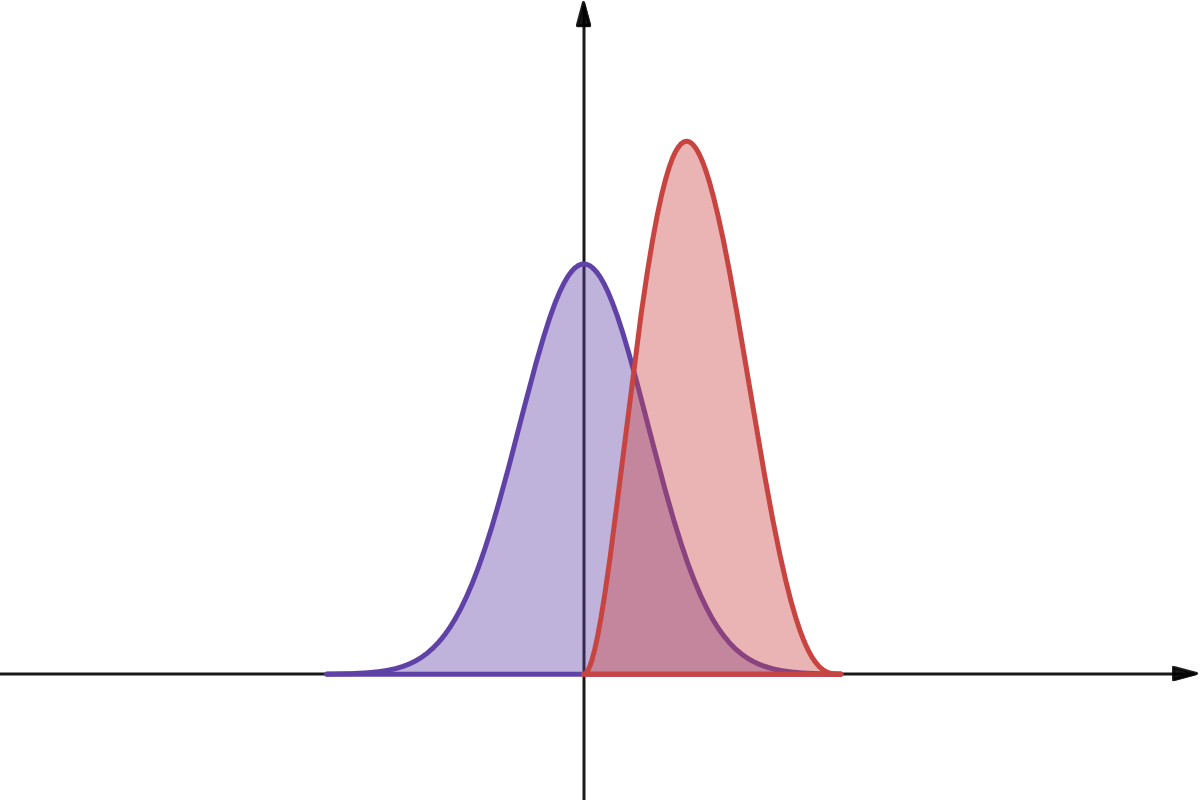
\includegraphics[width=\linewidth]{Figures/exnmodel_AB_cont.png}
	\end{subfigure} \begin{subfigure}{0.45\linewidth}
		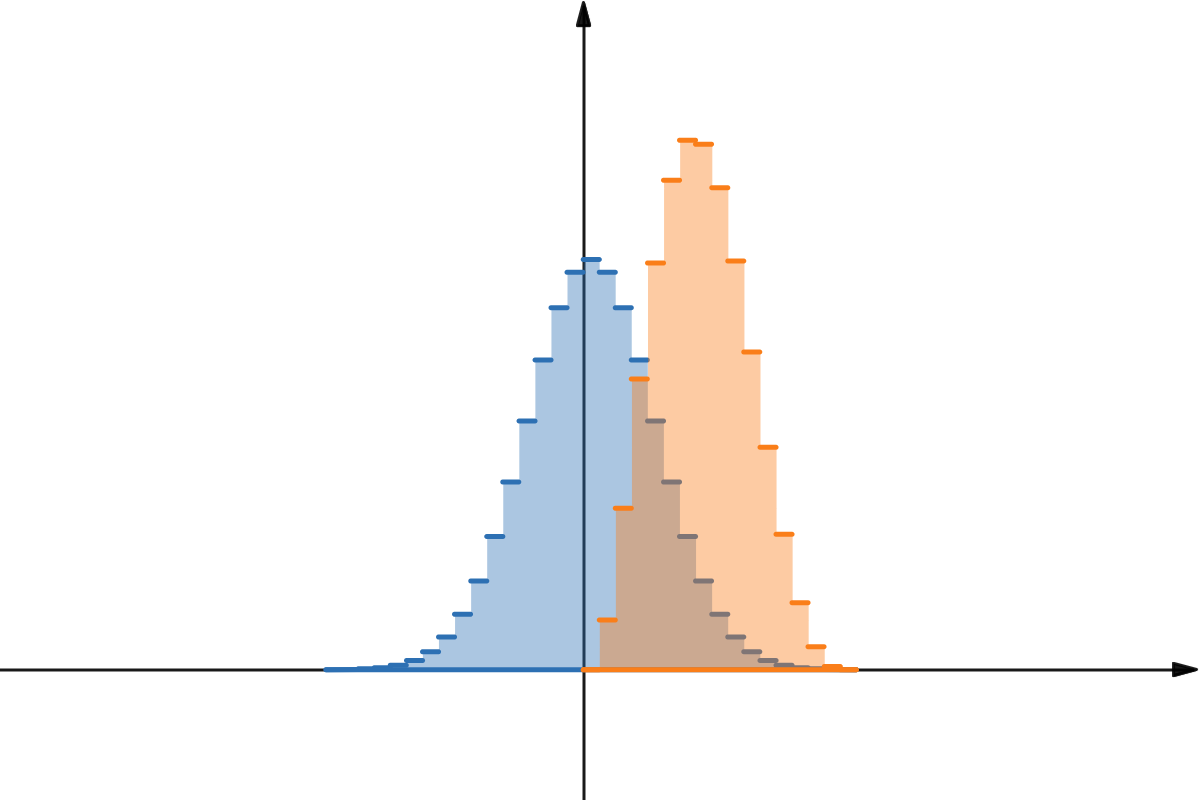
\includegraphics[width=\linewidth]{Figures/exnmodel_AB_disc.png}
	\end{subfigure}
\end{figure}

\noindent Now, let’s consider \cref{eq:SapAttribution_dist} and analyze the behavior of the estimated distance as the number of data points and the size of the boxes vary. By fixing the number of data points and decreasing the size of the boxes, the estimated distance gradually approaches $1$. This phenomenon occurs because there exists a critical dimension for $1 \;/ \; C$, such that with a sufficiently high probability, each sample becomes isolated within its own box. Consequently, this drives $J_{D_A,D_B}$ toward $0$, making each term in the summation equal to $1$.

\bigskip
In \cite{thesis}, the continuous nature of the $n$-tiles was addressed by discretizing the continuous space in which they were defined, fixing a resolution and applying posterization.\begin{toReview} Posterization is a process that reduces the number of discrete levels of color or intensity in an image, effectively mapping a continuous range of values into a smaller set of intervals. For example, in a color image, subtle variations in shades of red might all be grouped into a single pure red, removing the nuance of intermediate shades. \end{toReview} However, this approach results in a significant loss of information. Therefore, this paper will explore a method to achieve a cleaner and more dynamic discretization.

\section{Fuzzy clustering}
%La clusterizzazione fuzzy, nota anche come soft k-means, è una tecnica avanzata di analisi dei dati che consente ai punti dati di appartenere a più di un cluster. Questa modalità differisce dalla tradizionale clusterizzazione "hard", dove ogni punto dati è assegnato esclusivamente a un singolo cluster, utilizzando invece una logica fuzzy per determinare l'appartenenza di un dato a ciascun cluster. In altre parole, anziché avere un'affermazione binaria di appartenenza (1 o 0), si ha una misura continua di appartenenza che varia da 0 a 1. Questo è espresso attraverso una funzione di similarità, $\mu_x(C)$, che rappresenta il grado di appartenenza di un dato $x$ a un cluster $C$.
FFuzzy clustering, also known as soft k-means, is a data analysis technique that allows data points to be assigned to more than one cluster. Unlike traditional "hard" clustering, where each data point is assigned exclusively to a single cluster, fuzzy clustering employs fuzzy logic to determine the degree of membership for each data point within multiple clusters. Instead of a binary membership statement ($1$ or $0$), fuzzy clustering provides a continuous measure of membership that ranges from $0$ to $1$. This is represented by a similarity function, $\mu_x(C)$, which quantifies the degree to which a data point $x$ belongs to a cluster $C$.

% referenza K-Means
%La clusterizzazione fuzzy ha le sue radici nel lavoro di J.C. Dunn, che nel 1973 ha introdotto questo concetto come un'estensione dell'algoritmo di clustering k-means. Dunn ha evidenziato la maggiore precisione e robustezza della clusterizzazione fuzzy rispetto alla clusterizzazione rigida, soprattutto nella gestione dei dati anomali (outlier) \citep{FuzzyClustering_developDoc}.
\noindent Fuzzy clustering originated from the work of \citeauthor{FuzzyClustering_developDoc}, who introduced this concept as an extension of the $k$-means clustering algorithm in $1973$. \citeauthor{FuzzyClustering_developDoc} emphasized the increased accuracy and robustness of fuzzy clustering compared to hard clustering, particularly in handling anomalous data (outliers) \citep{FuzzyClustering_developDoc}.

% membership function
%L’algoritmo proposto da Dunn è detto Fuzzy C-Means Clustering (FCM) e si basa sull’utilizzo della tecnica Expectation-Maximization (EM) per definire la funzione di appartenenza ai cluster. Questa tecnica è un approccio iterativo per la stima dei parametri statistici, come ad esempio i centroidi dei cluster. Il processoEM si articola in due fasi principali:
%\begin{enumerate}
%    \item Expectation (E): In questa fase, viene formulata una funzione di verosimiglianza che esprime la probabilità che un dato appartenga a ciascun cluster in base alla sua distanza o similarità rispetto ai centroidi.
%    \item Maximization (M): Nella fase di massimizzazione, vengono individuati i parametri dei modelli che massimizzano la verosimiglianza, in questo caso i centroidi dei cluster, tramite un procedimento di ottimizzazione.
%\end{enumerate}
\noindent The algorithm proposed by \citep{FuzzyClustering_developDoc} is known as the \gls{fcm} and employs the \gls{em} technique to define the cluster membership function. This method is an iterative approach for estimating statistical parameters, such as cluster centroids. The \gls{em} process consists of two main steps:
\begin{enumerate}
    \item Expectation (E): In this phase, a likelihood function is formulated. This function expresses the probability that a data point belongs to each cluster, based on its distance or similarity to the centroids.
    \item Maximisation (M): In the maximization phase, an optimization procedure is used to identify the model parameters that maximize the likelihood, specifically the centroids of the clusters.
\end{enumerate}

%In sintesi, la clusterizzazione fuzzy offre una maggiore flessibilità rispetto alla clusterizzazione rigida, consentendo una rappresentazione più accurata e dettagliata dei dati, soprattutto in presenza di dati eterogenei o outlier.
\noindent In summary, fuzzy clustering provides greater flexibility compared to hard clustering, allowing for a more accurate and detailed representation of the data, particularly in the presence of heterogeneous data or outliers.

\subsection{Insights}
%Per comprendere appieno l'algoritmo \gls{fcm}, si definiranno preliminarmente i concetti fondamentali su cui si basa.
To fully understand the \gls{fcm} algorithm, we must first define the fundamental concepts on which it is based.

%\noindent I "punti dati" sono le osservazioni o le entità nel nostro insieme di dati, ognuna caratterizzata da una serie di attributi o feature. Questi punti dati possono essere visti come punti nello spazio multidimensionale, dove ogni dimensione corrisponde a un attributo specifico.
\noindent \textbf{Data points}: These are the observations or entities in our dataset, each characterized by a set of attributes or features. Data points can be viewed as points in a multidimensional space, where each dimension corresponds to a specific attribute.

%\noindent Una volta che abbiamo definito i punti dati, possiamo procedere a organizzarli in gruppi chiamati "cluster". Un cluster è una raccolta di punti dati che condividono caratteristiche simili tra loro. L'obiettivo dell'algoritmo di clustering è quello di raggruppare i punti dati in modo che quelli all'interno dello stesso cluster siano più simili tra loro rispetto a quelli in cluster diversi.
\noindent \textbf{Clusters}: Once we have defined the data points, we can organize them into groups called clusters. A cluster is a collection of data points that share similar characteristics. The goal of the clustering algorithm is to group data points so that those within the same cluster are more similar to each other than to those in different clusters.

%\noindent Ogni punto dati può essere associato a uno o più cluster attraverso la funzione di appartenenza a un cluster, indicata con $\mu_x$. Questa funzione assegna a ciascun punto dati un grado di partecipazione a ciascun cluster, rappresentato da un valore compreso tra $0$ e $1$. Ad esempio, se $\mu_x(C) = 1$, significa che il punto dati $x$ appartiene completamente al cluster $C$, mentre se $\mu_x(C) = 0.5$, significa che $x$ appartiene al cluster $C$ con una certa incertezza o ambiguità.
\noindent \textbf{Cluster Membership Function}: Each data point can be associated with one or more clusters through the cluster membership function, denoted as $\mu_x$, where $x$ represents a specific data point and $C$ represents a cluster. This function assigns each data point a degree of membership in each cluster, represented by a value between $0$ and $1$. For example, if $\mu_x(C) = 1$, it indicates that data point $x$ belongs completely to cluster $C$. Conversely, if $\mu_x(C) = 0.5$, it suggests that $x$ has some degree of uncertainty or ambiguity in its membership to cluster $C$.
\begin{notation}
Denote:
\begin{itemize}
\item the dataset with \\ $\mathcal{S} = (x_i)_{i=1:N}$ where $x_i\in\mathbb{R}^K$
\item the set of cluster centroids with \\ $\mathcal{C}={C_1,\dots,C_M}$ where $C_j\in\mathbb{R}^K$
\item the weight matrix with \\ $U=(u_{ij})$ dove $u_{ij}=\mu_{x_i}(C_j)$
\item the quadratic Euclidean distance matrix with \\ $D^2=(d^2_{ij})$ where $d_{ij}=\|x_i-C_j\|^2$
\end{itemize}
\end{notation}

\begin{exempli_gratia}
To understand the meaning of data points and clusters, let us consider the following example:

\noindent Imagine we need to classify the apples transported by a lorry into two color categories: green and red. However, within this set, there might also be yellow apples. The $k$-means algorithm would treat a yellow apple as an anomaly compared to the red and green apples. In contrast, fuzzy clustering quantifies this anomaly by asserting that a yellow apple is a blend of red and green.

\noindent The colours of the apples can be represented in a one-dimensional space. In this space, we observe a distribution of data points showing green and red at the extremes, with yellow apples located in the center.

\noindent Clusters, in the context of fuzzy logic, are sets defined by centroids representing specific shades of colour, which are not necessarily present in the set of data points. For example, if there are red and green apples, there are actually two centroids representing specific shades of red and green, even though there are no apples with such colour shades.

\begin{center}
	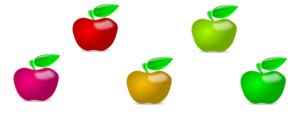
\includegraphics[width=0.5\linewidth]{Figures/apple.png}
\end{center}
\end{exempli_gratia}

\begin{remark}
	The \gls{fcm} algorithm recognizes that real-world data may contain errors or uncertainties. Instead of rigidly assigning each data point to a single cluster, it introduces a measure of uncertainty in the assignment. This approach results in assigning a fuzzy degree of membership to each point concerning each cluster, rather than relying on a binary classification.
\end{remark}

\begin{definition}[membership measure]\label{def:fuzzy}
	Given a point $x$ and a cluster $C$, the membership measure $\mu_x(C)$ is proportional to the inverse of the square of the Euclidean distance between the point $x$ and the centroid of the cluster $C$, i.e. $\frac{1}{\|x-C\|^2}$.\\ We assume that the sum of the membership measures of $x$ to all clusters in the set $\mathcal{C}$ is equal to $1$:
	$$\sum_{C\in\mathcal{C}}\mu_x(C)=1 \quad \forall x$$
	Consequently, the membership measure $u_{ij}$ of point $x_i$ to cluster $C_j$ is computed as:
	$$u_{ij} = \frac{1}{\sum_{k}\frac{d^2_{ij}}{d^2_{ik}}}$$
\end{definition}
\begin{remark}
	The \gls{kmeans} algorithm, which is based on Boolean logic, seeks to minimise the sum of the squared distances between each data point and the centroid of the cluster to which it is assigned. In other words, the goal of the \gls{kmeans} algorithm is to minimise the sum of intra-cluster variances, where the variance of a cluster is defined as the sum of the squared distances between each point in the cluster and the cluster centroid.

	\noindent Formally, the goal of the \gls{kmeans} algorithm can be expressed as:
	\begin{equation*}
		\text{argmin}_\mathcal{C}\left[\sum_{C\in\mathcal{C}}\sum_{x \in C}\|x-C\|^2\right]
	\end{equation*}
	\noindent In the case of fuzzy clustering, the membership of a point in a cluster is expressed by a fuzzy measure instead of a Boolean logic. The objective function of the \gls{kmeans} method can be rewritten equivalently with membership measures:
	\begin{equation*}
		\sum_{C\in\mathcal{C}}\sum_{x \in \mathcal{S}}\delta_x(C)\|x-C\|^2
	\end{equation*}
	where $\delta_x(C)$ represents the membership measure of point $x$ in cluster $C$. This objective function reflects the weighting of the squared distances by the membership measure of each point in the clusters.
\end{remark}
\begin{definition}[Loss function and cluster weight]
	We define the fuzzy clustering loss function from the \gls{kmeans} algorithm as follows:
	\begin{equation}
		L_\mathcal{S}(\mathcal{C}) := \sum_{C\in\mathcal{C}}p_\mathcal{S}(C) := \sum_{C\in\mathcal{C}}\sum_{x \in \mathcal{S}}\mu_x(C)^2\|x-C\|^2
		\label{eq:loss}
	\end{equation}
	where $p_\mathcal{S}(C)$ is the sum of the squared distances between the points in the cluster $C$ and its centroid. This loss function is coercive on the centroids, which means that it tends to infinity when the centroids recede to infinity, and has a finite lower bound when the centroids are bound to a compact set in the data space. For this reason we know that there is a global minimum although the uniqueness of local minima is not guaranteed.\footnote{for more about coercitive functions, see \\ \url{https://www1.mat.uniroma1.it/people/lanzara/OTT0708/Ottimizzazione0708.pdf}}
\end{definition}
\begin{remark}
	The \gls{kmeans} algorithm and fuzzy clustering via \gls{fcm} share a similar approach in updating of cluster centroids. Both algorithms aim to find the optimal position of the centroids that minimizes the loss function based on the distances between the data points and the centroids themselves.

	\noindent In the \gls{kmeans} algorithm, the process of updating centroids occurs iteratively. Initially, centroids are randomly assigned to clusters. Data points are then assigned to the nearest clusters (based on Euclidean distance), after which the centroids are updated by averaging the points assigned to each cluster. This process is repeated until the centroids converge to stable positions.

	\noindent Similarly, the \gls{fcm} algorithm iteratively updates both the centroids of the clusters and the cluster membership measures for the points. In each iteration, the optimal centroids for a given configuration of membership measures are determined, and vice versa, until a stable configuration is reached that minimizes the loss function defined based on the membership measures and the distances between the data points and the centroids.
\end{remark}

\bigskip
\begin{theorem}[Update formula 'M']
	\label{thm:Mupdate}
    Fixed the matrix $U$, the optimisation of \cref{eq:loss} finds its minimum in the centroids according to the following update formula:
    \begin{equation}
        C^{\texttt{new}}_j = \frac{\sum_{i=1}^Nu_{ij}^2x_{i}}{\sum_{i=1}^Nu_{ij}^2} \text{\hspace{1cm}} \forall j
    \end{equation}
	\begin{proof}
	    Fixed the matrix $U$, the loss function is differentiable, convex and coercive. Consequently, to find the global minimum of the function, it is sufficient to find the points where the gradient is null.

	    \noindent Calculating the partial derivatives of the gradient with respect to the centroids $C_j$, we obtain:
	\begin{equation*}
	    \frac{\partial}{\partial C_{j}} L_\mathcal{S}(\mathcal{C}) = \frac{\partial}{\partial C_{j}} p_\mathcal{S}(C_j) = \sum_{i=1}^N\frac{\partial}{\partial C_{j}} u_{ij}^2\|x_i-C_j\|^2 = 2\sum_{i=1}^N u_{ij}^2\left(C_{j}-x_{i}\right)
	\end{equation*}

	\noindent The gradient is null when all partial derivatives are null, which implies:
	\begin{equation*}
	    \sum_{i=1}^N u_{ij}C^{\text{new}}_{j} = \sum_{i=1}^N u_{ij}x_{i} \quad \forall j
	\end{equation*}

	\noindent Since $C^{\text{new}}_j$ does not depend on the index $i$, the thesis is proved.
	\end{proof}
\end{theorem}

\begin{remark}
	The calculation of the centroid update formula in fuzzy clustering is closely tied to the concept of parameter estimation through the maximum likelihood method. Specifically, it involves maximizing the joint density of the data and model parameters, conditional on the assignment of points to clusters.
	The density to be maximized is given by:
	\begin{equation*}
	    f_U(\mathcal{S}|\mathcal{C}) \propto \prod_{i,j}\text{exp}\left[-u_{ij}^2\frac{\|x_i-C_j\|^2}{2}\right]
	\end{equation*}
	where $f_U(\mathcal{S}|\mathcal{C})$ is the joint density of the points conditioned on the set of centroids where $u_{ij}$ is the membership measure of point $x_i$ in cluster $C_j$.

	\noindent The density of the single sample $x_i$ is:
	\begin{equation*}
	    f_U^i(x_i|\mathcal{C}) \propto \prod_{j}\text{exp}\left[-u_{ij}^2\frac{\|x_i-C_j\|^2}{2}\right]
	\end{equation*}
	where $f_U^i(x_i|\mathcal{C})$ is the density of the observed datum $x_i$ conditioned on the centroids.

	\noindent The goal is to maximise the likelihood density in order to obtain accurate estimates of the model parameters, which in the context of fuzzy clustering are represented by the cluster centroids. For this reason, the algorithm is classified as \gls{em} because the phase \verb"E" sets the densities for maximum likelihood when the matrix $U$ is defined and the phase \verb"M" solves the problem by finding the centroids that best explain the model.
\end{remark}

The \cref{alg:FuzzyClustering} computes the ideal centroids in fuzzy clustering and does not directly aim to minimise of \cref{eq:loss}, but rather to iteratively updates the centroids and membership measures until a stable configuration is reached that best represents the input data.

\begin{algorithm}[h]
\caption{Fuzzy Clustering\\
	\textsc{INPUT}\\
	$\bullet$ $\mathcal{S}$: set of data $x_1,\cdots,x_N$\\
	$\bullet$ $\mathcal{C}$: centroids $C_1,\cdots,C_j$}
\begin{algorithmic}[1]
\Procedure{FuzzyClustering}{$\mathcal{S}, \mathcal{C}$}
    \While{not reached the exit criterion}
        \State $D^2 \gets (d^2_{ij})$ with $d_{ij}=\|x_i-C_j\|^2$
        \State $U^2 \gets (u_{ij}^2)$ with $u_{ij}=\left(\sum_{k}D^2_{ij}/D^2_{ik}\right)^{-1}$
        \Comment{see \cref{thm:Mupdate}}
        \For{$j \gets 1$ to $M$}
            \State $C^\text{new}_j \gets \sum_{i=1}^N x_iU^2_{ij} / \sum_{i=1}^N U^2_{ij}$
        \EndFor
    \EndWhile
\EndProcedure
\end{algorithmic}
\label{alg:FuzzyClustering}
\end{algorithm}

\subsection{Implications}
This algorithm is particularly effective for clustering problems that involve noise. Two other well-known methods operate on different paradigms: \gls{kmeans} and \gls{gmm}.

\paragraph{\gls{kmeans}} is a fundamental clustering algorithm that partitions data points into disjoint groups, where the centroids represent the mean of each group. Its primary goal is to minimize the sum of variances within these groups, resulting in well-defined clusters.

\paragraph{\gls{gmm}} is a more sophisticated algorithm based on the assumption that the data points are generated by a specific statistical process:
\begin{itemize}
    \item[1] Select with probability $p_j$ the $j$-th cluster.
    \item[2] Generate a random data point from $\mathcal{N}(C_j, \Sigma_j)$.
\end{itemize}
This method not only tries to find clusters and label data points, but also proposes normal distributions with averages $\mathcal{C}$ and covariances $\Sigma$, assigning probabilities indicating the weight of each cluster. It is possible to label the data points using the Mahalanobis distance\footnote{For more information on the Mahalanobis distance, see \url{https://en.wikipedia.org/wiki/Mahalanobis_distance}}.

\bigskip
Next, lets see how these methods behave in the presence of noisy data. Specifically, $6$ random centroids were chosen in a two-dimensional space, from which $20$, $20$, $20$, $30$, $30$ and $40$ data points with different covariance matrices were generated, respectively. In addition, uniformly generated noisy data points were added, constituting $30\%$ of the total (i.e. $48$ noisy data points). A representation of this data can be seen in \cref{fig:data_true}. As can be seen, noise can create \textit{outliers}, i.e. distant points that would be better ignored to achieve good clustering.

\begin{figure}[ht]
    \centering
    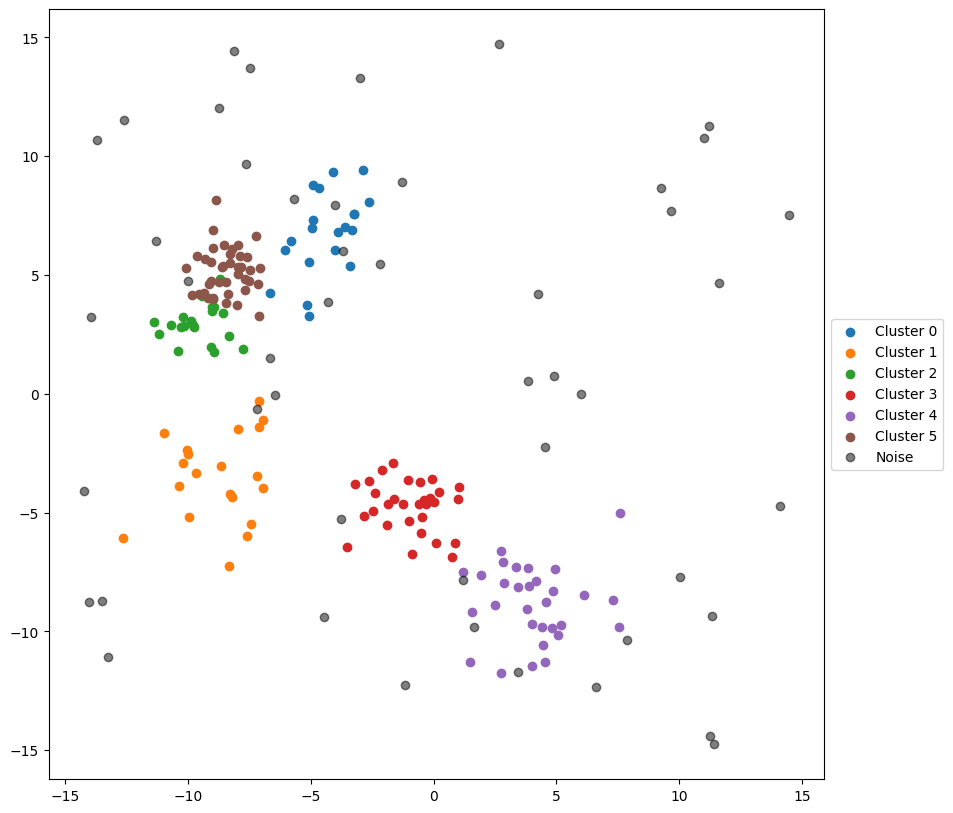
\includegraphics[width=0.9\linewidth]{Figures/dati_veri.png}
    \caption[example of data for clustering]{Data points are coloured according to their label, while noise is shown in grey.}
    \label{fig:data_true}
\end{figure}

\noindent Now let will try clustering with \gls{kmeans} using the right number of centroids, i.e. $6$. In \cref{fig:data_kmeans} we can see that the noise has created an additional cluster and two of the original clusters have merged into one. Although the result is quite satisfactory, it is not entirely clean.

\noindent Next, let is apply clustering with \gls{gmm} again using $6$ centroids. In \cref{fig:data_gmm} it can be seen that the weight of the cluster generated by the noise is very small. Furthermore, the covariance matrices allow the position of the centroids to be calculated more precisely, providing information on the nature of the clusters and creating a hierarchical structure. This is because, in reality, these are not real clusters, but normal distributions.

\noindent Finally, let clustering be applied with \gls{fcm} using $6$ centroids. In \cref{fig:data_fcm} we observe that the centroids are less affected by noise, making it possible to identify which data are potentially noisy or shared between several clusters.

\bigskip
We have observed that in the presence of noise, the algorithm \gls{fcm} can be very useful. However, the algorithm \gls{gmm}, although computationally onerous, also provides very valuable information about the nature of the data. In this thesis, we will use the \gls{fcm} algorithm to reduce the amount of information to be processed and the \gls{kmeans} algorithm for efficient initialisation of centroids.

\section{\gls{dft}}
\begin{modified}
The \gls{dft} is a powerful tool for analyzing signals in the frequency domain, often used in applications such as signal processing, image analysis, and data compression. Its ability to transform spatial or temporal data into frequency components makes it particularly effective for isolating patterns or removing noise. In this thesis, the \gls{dft} will be used to compress and clean images during the pre-processing phase, which will be discussed in detail in \cref{chap:methodology}.
\end{modified}
\begin{note}
	Nell'introduzione della tesi sarà già accennato cosa è il pre-process a grandi linee. Poi in methodology sarà descritto meglio
\end{note}

\noindent This procedure, known as spectral analysis, makes it possible to study signals, waves, vibrations, sounds and images. In addition to these areas, DFT also has major scientific applications, such as the precise estimation of sunspot cycles, helping to predict and control phenomena such as geomagnetic storms\footnote{For more about geomagnetic storms and them correlation with sunspot, see \url{https://en.wikipedia.org/wiki/Geomagnetic_storm}}.

\subsection{Insights}
\begin{modified}
	The \gls{dft} is a discrete analogue of the \gls{cft}, which represents a function in terms of its frequency components. More rigorously, given a function $f\in L^1(\mathbb{R})$, its Fourier transform is a functional operator, denoted by $\mathcal{F}$, which associates $f$ with its frequency representation:
	\[
		\mathcal{F}(f): \omega \mapsto \int_{\mathbb{R}} e^{-i2\pi \omega x}f(x)\,dx
	\]
	\begin{note}
		La periodicità di $f$ è richiesta solo nelle serie?
	\end{note}

	\noindent By contrast, the Fourier series applies specifically to periodic functions, representing them as an infinite sum of sine and cosine waves with discrete frequencies. In this context, the \gls{dft} can be viewed as a finite approximation of the Fourier series, applied to sampled data over a finite interval.
\end{modified}

\noindent The \textbf{Fourier inversion theorem} states that, if both $f$ and $\mathcal{F}(f)$ belong to $L^1(\mathbb{R})$ (i.e. they are both integrable), then for almost any $x\in\mathbb{R}$ it is possible to recover $f(x)$ via the following inverse relation:
\[
f(x)=\int_{\mathbb{R}}{\mathcal{F}\left(f\right)}(\omega)e^{i2\pi x\omega}\,d\omega
\]
In other words, the Fourier transform and its inverse allow switching back and forth between the time (or space) and frequency domains.

\bigskip
The discrete version of this transform, namely \gls{dft}, is used to analyse signals sampled at regular intervals. Thus, while \gls{cft} works on continuous signals, \gls{dft} applies to finite and discrete signals, making it suitable for digital signal processing.

\noindent To better understand how \gls{dft} gives information about the amplitudes and phases of the different frequencies that make up a sequence, it is useful to introduce the Fourier coefficients. These coefficients make it possible to decompose a data sequence into sinusoids associated with different frequencies.

\begin{modified}
\begin{remark}
	The Fourier coefficients of the sequence $(x_n)_{n=0}^{N-1}$ is a sequence of complex numbers $(X_k)_{k=0}^{N-1}$ such that:
	\begin{equation}
		x_n = \frac{1}{N}\sum_{k=0}^{N-1} X_k e^{i2\pi\frac{k}{N}n}
	\end{equation}

	\noindent In the follow examples, we want show an intuitive relation between Fourier coefficients and them time series. It is very important to interpretate a result of a \gls{dft}.
\end{remark}
\end{modified}

\begin{exempli_gratia}[Amplitude]
	\begin{toReview}
		In this example we understand how the Fourier coefficients determine the amplitude of a frequency.
	\end{toReview}

	\noindent Take a time series consisting of $N$ complex numbers, described by the following coefficients:
	\[
		X_0=0,\;X_1=A,\;X_2=0\;\cdots\;X_{N-2}=0,\;X_{N-1}=A
	\]
	From these coefficients we obtain the time series:
	\[
		x_n = \frac{1}{N}A\left(e^{i2\pi \frac{n}{N}} + e^{i2\pi \frac{n}{N}(N-1)}\right) = \frac{2A}{N}\cos\left(2\pi\frac{n}{N}\right)
	\]
	\begin{modified}
	We note that the series is only a sinusoidal function, with amplitude $\frac{2A}{N}$ and frequency $\frac{2\pi}{N}$.
	\begin{center}
		\centering
		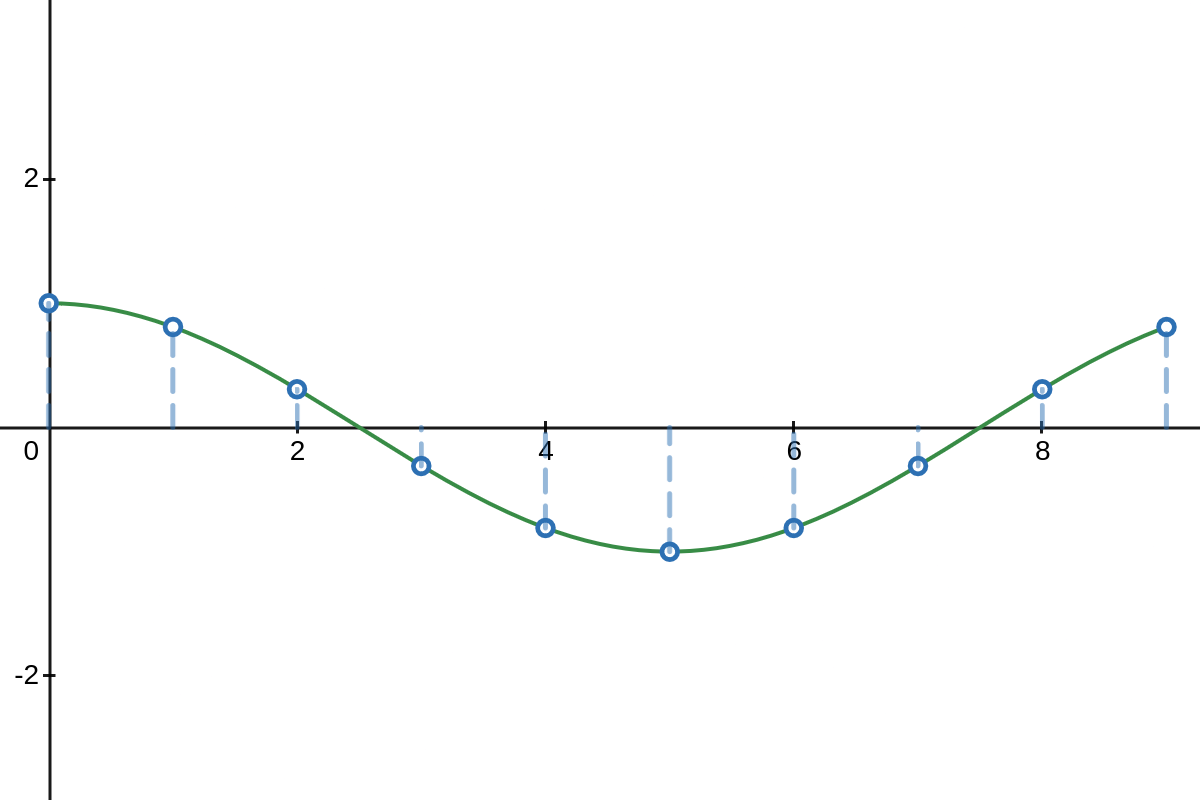
\includegraphics[width=0.5\textwidth]{Figures/fftexample1.png}
	\end{center}
	\end{modified}
\end{exempli_gratia}

\begin{exempli_gratia}[Frequency]
	\begin{toReview}
		In the previous example the significant frequency is $2\pi\frac{n}{N}$, in this example we study how to refer to a different frequency.
	\end{toReview}

	\noindent Take a time series consisting of $N$ complex numbers, described by the following coefficients:
	\[
		X_p=A,\;X_{N-p}=A
	\]
	where all other values are zero.

	\noindent The generated time series will be:
    \[
		x_n = \frac{1}{N}A\left(e^{i2\pi \frac{n}{N}p} + e^{i2\pi \frac{n}{N}(N-p)}\right) = \frac{2A}{N}\cos\left(2\pi\frac{n}{N}p\right)
	\]
	\begin{modified}
	As can be seen, the coefficients refer to the amplitude of a certain frequency indicated by the index of Fourier coefficient.
	\begin{center}
		\centering
		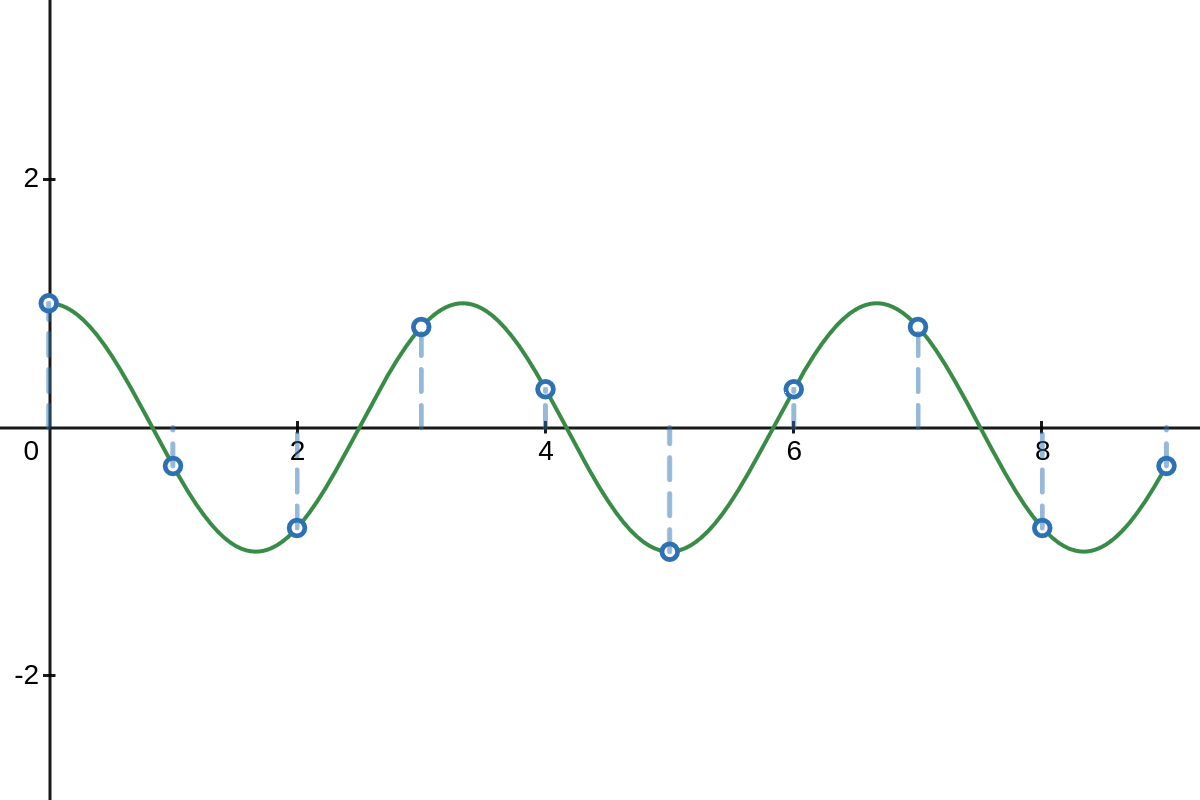
\includegraphics[width=0.5\textwidth]{Figures/fftexample2.png}
	\end{center}

	\noindent If we have $X_1=A, X_{N-1}=A$, $X_2=B, X_{N-2}=B$, then we will obtain time series:
	\[
		x_n = \frac{2A}{N}\cos\left(2\pi\frac{n}{N}\right) + \frac{2B}{N}\cos\left(2\pi\frac{n}{N}2\right)
	\]
	\end{modified}
\end{exempli_gratia}
\begin{exempli_gratia}[Phase]
	\begin{toReview}
		In the previous example we observed that the index of the Fourier coefficient refers to a specific frequency. Now we are going to see how the Fourier coefficients derive the phase of a frequency in a time series.
	\end{toReview}

	\noindent Take a time series consisting of $N$ complex numbers, described by the following coefficients:
	\[
		X_0=0,\;X_1=Ae^{i\theta},\;X_2=0,\;\dots,\;X_{N-2}=0,\;X_{N-1}=Ae^{-i\theta}
	\]
	The resulting time series will be:
    \[
		x_n = \frac{2A}{N}\cos\left(\frac{2\pi}{N}n + \theta\right)
	\]
	Here, the modulus of the coefficient describes the amplitude of the frequency, while its argument $\theta$ describes its phase.
	\begin{center}
		\centering
		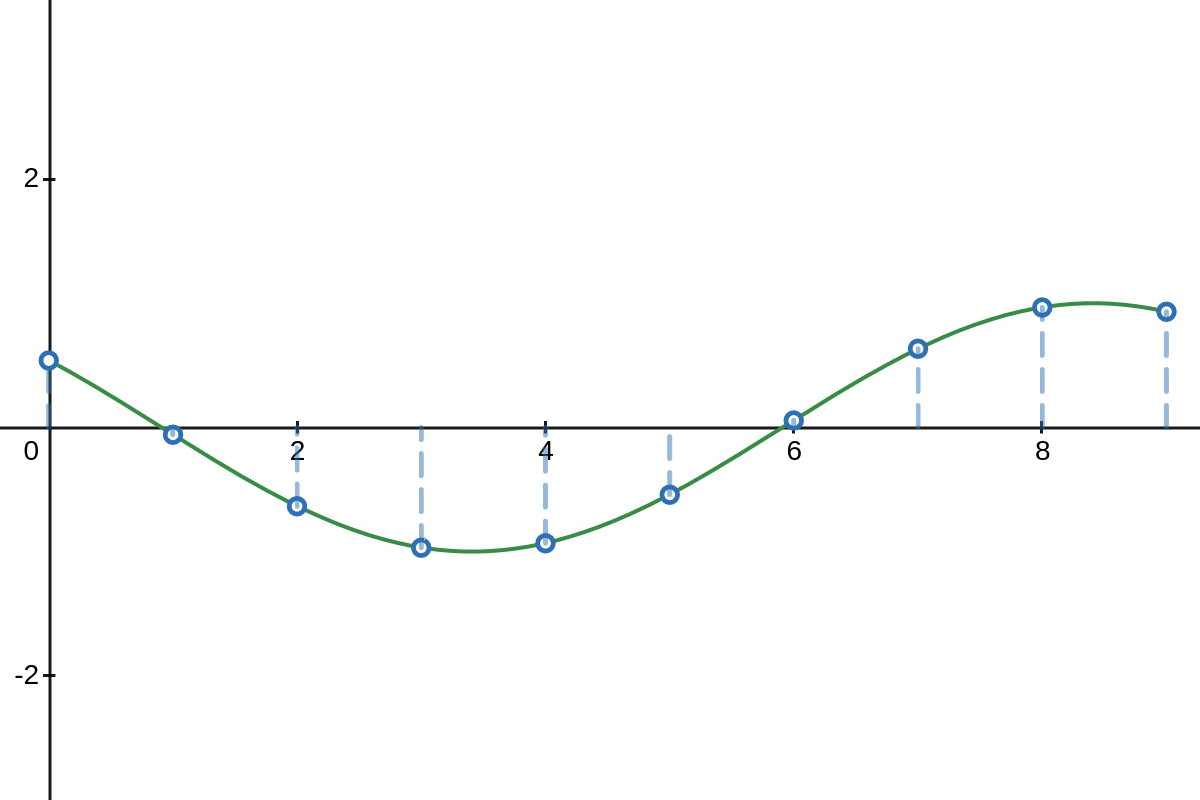
\includegraphics[width=0.5\textwidth]{Figures/fftexample3.png}
	\end{center}

	\begin{modified}
		\noindent We observe also that to ensure that the series is real, the opposite coefficient must be the conjunct of $X_1$.
	\end{modified}
\end{exempli_gratia}

\bigskip
We now ask ourselves whether it is possible to estimate the Fourier coefficients from a time series.
\begin{proposition} \label{prop:dft_unitaria}
	The matrix $\frac{1}{\sqrt{N}}\left(e^{i2\pi\frac{k}{N}n}\right)_{n,k=0}^{N-1}$ is unitary.
	\begin{proof}
		\begin{modified} We prove the thesis by studying the inner product between two rows of the matrix: \end{modified}
		\[
		\frac{1}{N}\sum_{k=0}^{N-1} e^{i2\pi\frac{k}{N}n}\cdot e^{-i2\pi\frac{k}{N}m} = \frac{1}{N}\sum_{k=0}^{N-1} e^{i2\pi\frac{k}{N}(n-m)}
		\]
		If $n = m$, the result of the sum is $1$. Else if $n \neq m$, we obtain:
		\[
			\frac{1}{N}\sum_{k=0}^{N-1} e^{i2\pi\frac{k}{N}(n-m)} = \frac{1}{N}\frac{e^{i2\pi\frac{N}{N}(n-m)}-1}{e^{i2\pi\frac{1}{N}(n-m)}-1} = 0
		\]
		This proves that the matrix is unitary.
	\end{proof}
\end{proposition}

\bigskip
Proving that the matrix $\frac{1}{\sqrt{N}}(e^{i2\pi\frac{k}{N}n})_{n,k=0}^{N-1}$ is unitary is extremely relevant to the computation of Fourier coefficients.
\begin{theorem}[\gls{dft}]
	The Fourier coefficients of the time series $(x_n)_{n=0}^{N-1}$ are given by the formula:
	\begin{equation}
		X_k = \sum_{n=0}^{N-1} x_n e^{-i2\pi\frac{n}{N}k}
	\end{equation}
	\begin{proof}
		Define $U$ as matrix $\frac{1}{\sqrt{N}}(e^{i2\pi\frac{k}{N}n})_{n,k=0}^{N-1}$

		\noindent By definition of the discrete Fourier transform, we can write $\vec{X} = \frac{1}{\sqrt{N}}U\vec{x}$, where $\vec{X}$ is the vector of Fourier coefficients and $\vec{x}$ is the vector of the original time series.

		\noindent As shown in \cref{prop:dft_unitaria}, the matrix $U$ is unitary, so it admits an inverse, which is its transposed conjugate $U^H$. \\
		Therefore, we can invert the transformation and obtain:
		\[
			\vec{x} = \sqrt{N}U^H\vec{X}
		\]

		\noindent This relation allows us to get the Fourier coefficients from the time series.
	\end{proof}
\end{theorem}

\begin{definition}[Fourier coefficient]
	We define Fourier coefficient of the time series $(x_n)^{N-1}_{n=0}$ is the sequence of complex numbers $(X_k)^{N-1}_{k=0}$:
	\[
		X_k = \sum_{n=0}^{N-1} x_n e^{-i2\pi\frac{n}{N}k}
	\]
\end{definition}

\subsection{Implications}
The possibility of calculating Fourier coefficients directly by means of a simple matrix-vector product not only makes the analysis very informative, but also easily achievable.

\begin{modified}
\paragraph{\gls{fft}} The computational cost of the matrix-vector product for computing Fourier coefficients is $O(N^2)$, which is not excessive in itself. However, there are better algorithms that compute Fourier coefficients and that reduce this cost. An example is \gls{czt} algorithm of \citet{czt_source} with computational cost $O(N\log N)$. An other example is the algorithm of \citet{FFT} showed in \cref{alg:fft}, which use a technique of \textit{divide et impera} to compute Fourier coefficients.
\begin{remark}
	The \cref{alg:fft} uses an important property of \gls{fft}: when $N=N_1\times N_2$ with $N_1, N_2> 1$ we can \textit{divide} the input sequence, \textit{impera} over them and, finally, merge results to obtain the desiderate Fourier coefficients.

	\noindent Let $x=(x_i)_{i=0}^{N-1}$ a time series, we compute these Fourier coefficients:
	\begin{itemize}
		\item $X^{0}$ are the Fourier coefficients of  $\left(x_{N_2k}\right)_k$ with $N_1$ values.
		\item $X^{1}$ are the Fourier coefficients of $\left(x_{N_2k+1}\right)_k$ with $N_1$ values.
		\item $\cdots$
		\item $X^{N_2-1}$ are the Fourier coefficients of $\left(x_{N_2k+N_2-1}\right)_k$ with $N_1$ values.
	\end{itemize}
	Now we use them to compute $X$:
	\begin{align*}
		X_k &= \sum_{n=0}^{N-1} x_n e^{-i2\pi\frac{n}{N}k} = \sum_{p=0}^{N_2-1}\sum_{l} x_{N_2l+p} e^{-i2\pi\frac{N_2l+p}{N}k} \\
		&= \sum_{p=0}^{N_2-1}\sum_{l} x_{N_2l+p} e^{-i2\pi\frac{N_2l}{N}k}e^{-i2\pi\frac{p}{N}k} \\
		&= \sum_{p=0}^{N_2-1}e^{-i2\pi\frac{p}{N}k}X^p_k
	\end{align*}
	In particular, the \cref{alg:fft} uses the case of $N_2=2$ and the follow observation:
	\begin{align*}
		X_{k+N/2} &= \sum_{n=0}^{N-1} x_n e^{-i2\pi\frac{n}{N}\left({k+N/2}\right)} = \sum_{n=0}^{N-1} x_n e^{-i2\pi\frac{n}{N}k -i2\pi\frac{n}{2}} \\
		&= \sum_{l} x_{2l} e^{-i2\pi\frac{2l}{N}k -i2\pi l} + \sum_{l} x_{2l} e^{-i2\pi\frac{2l+1}{N}k -i2\pi\frac{2l+1}{2}} \\
		&= X^0_k - e^{-i2\pi\frac{1}{N}k}X^1_k
	\end{align*}
\end{remark}
\noindent The computational cost of \cref{alg:fft} is $O(N\log N)$ if the base case (when $N$ is not even, or in general is a prime) has cost $O(N\log N)$.
\end{modified}

\begin{algorithm}[h]
	\caption[\gls{fft} algorithm]{\citet{FFT} \& \gls{czt} algorithms.\\
		\begin{minipage}[t]{\linewidth}
			\textsc{INPUT}
			\begin{itemize}[noitemsep, topsep=0pt]
				\item[$x$:] time series $x_1,\dots,x_N$
			\end{itemize}
			\textsc{OUTPUT}
			\begin{itemize}[noitemsep, topsep=0pt]
				\item[$X$:] Fourier coefficients of $x$
			\end{itemize}
		\end{minipage}
	}
	\begin{algorithmic}[1]
		\Function{FFT}{$x$}
		\If{$N$ is odd} \Return $\Call{CZT}{x}$ \Comment base case
		\EndIf

		\State $\text{even} \gets \Call{FFT}{\left[x_0,x_2,\cdots,x_{N-2}\right]}$
		\State $\text{odd} \gets \Call{FFT}{\left[x_1,x_3,\cdots,x_{N-1}\right]}$

		\State $X$ is an array of size $N$

		\For{$k\in 0,\dots,\frac{N}{2}-1$}
			\State $t \gets \exp\left(-2\pi i k / N\right)\cdot \text{odd}[k]$
			\State $X[k] \gets \text{even}[k] + t$
			\State $X[k + N/2] \gets \text{even}[k] - t$
		\EndFor
		\State \Return $X$
		\EndFunction
	\end{algorithmic}
	\label{alg:fft}
\end{algorithm}

\begin{modified}
\paragraph{Periodogram} The periodogram is a practical tool that graphically represents the amplitude of the different frequencies composing a time series, providing insight into the frequency spectrum of the signal. By visualising the power associated with each frequency, it highlights the dominant components of the spectrum, making it particularly useful for distinguishing between noise and significant frequencies. This connects directly to the theory of the \gls{dft}, as the periodogram is derived from the squared modulus of the Fourier coefficients, representing the signal's energy distribution across frequencies.

\noindent To illustrate this, we apply the \gls{dft} to the \texttt{sunspots} dataset from the \gls{r} package, which contains the number of sunspots observed each month from $1749$ to $1984$. Sunspots are known to correlate with the Sun's magnetic activity, which is believed to exhibit periodic cycles. Using the periodogram, we aim to identify these cycles, particularly the dominant periodic components in the data, and evaluate their significance compared to noise.
\begin{figure}[ht]
	\centering
	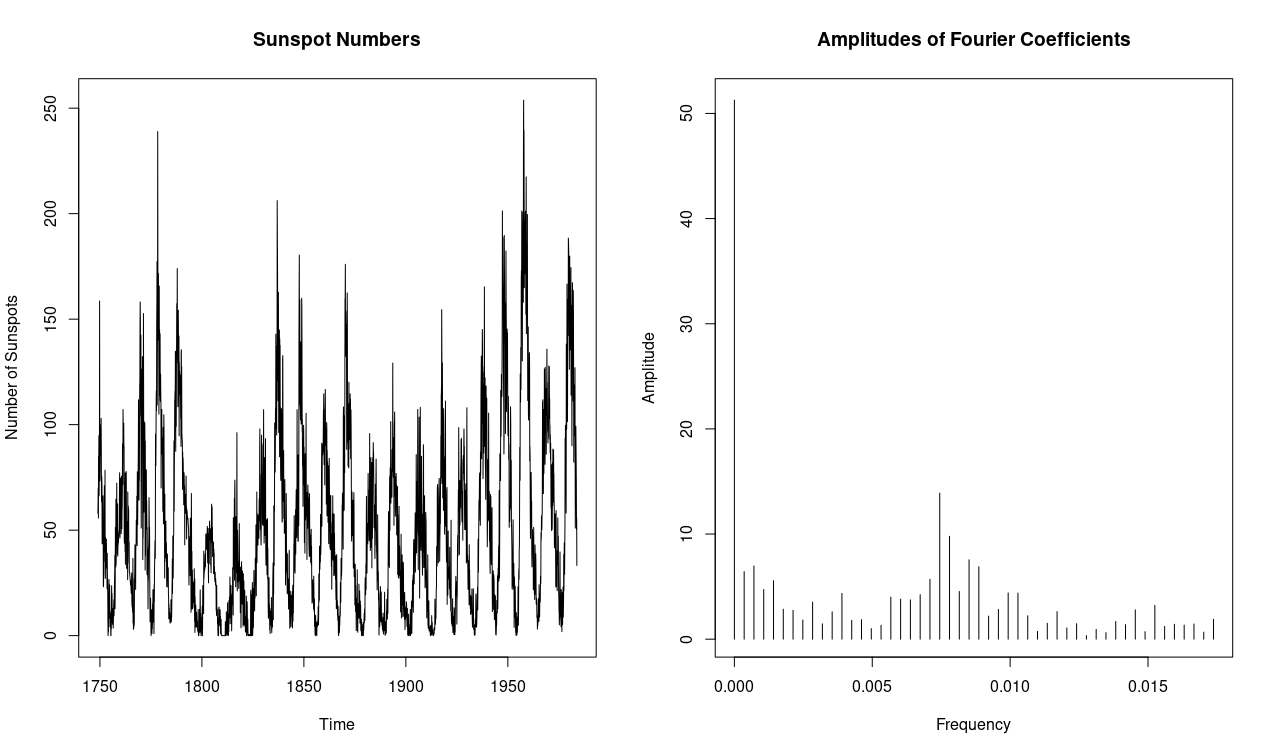
\includegraphics[width=\textwidth]{Figures/sunspots.png}
	\caption[Periodogram of sunspots]{On the left, the time series of the number of sunspots recorded each month from $1749$ to $1984$ (\(N = 2820\)). This representation shows the variation of sunspots over time, highlighting any cycles. On the right, the periodogram obtained by applying the \gls{dft} to the time series. Each point represents the squared modulus of a Fourier coefficient, which measures the energy associated with a given frequency. We can see a peak at frequency $0$, corresponding to the sum of the values of the time series (\(X_0 = \sum_{n=0}^{N-1} x_n\)).}
\end{figure}
\end{modified}

\noindent Looking at the periodogram obtained with \gls{fft}, we observe that some frequencies are much more pronounced than others. In particular, the frequency $\approx 0.0075\operatorname{\mathrm{Hz}}$ (corresponding to about a cycle of $135$ months) indicates a cycle of about $11$ years, which confirms what is already known about the cyclic nature of solar activity.

\noindent This example demonstrates how the DFT is a powerful tool for detecting and analysing periodic patterns in observational data. The use of the periodogram not only makes it possible to identify the main frequencies, but also to evaluate their relative importance respect to the background noise.

\begin{note}
	"Di qual è lo scopo della tesi mi sembra che tu non abbia parlato. Immagino ci sarà nell'introduzione? Ma in ogni caso, in apertura di questo capitolo dovresti anticipare di cosa si parlerà e perché"

	\bigskip \noindent Sì ci sarà nell'introduzione della tesi e ho messo un accenno al suo ruolo nell'introduzione della sezione DFT in queste correzioni
\end{note}

\section{Application}
\begin{modified}
In this section, we will develop specific applications of the topics discussed in this chapter to see how they can be used in the context of this thesis. The discussion will focus on the use of fuzzy clustering to address the problem of continuity in colour space, the practical implementation of the \gls{fcm} algorithm, and the use of \gls{fft} for image analysis.
\end{modified}
\subsection{Comparing works, the idea of clustering}
\begin{modified}
As we have seen, the tiles used to compute \cref{eq:SapAttribution_dist} can be represented as sequences of real numbers. However, their continuous nature introduces a problem in the computation of comparison values, since it reduces the $n$-grams to unique and unrepeatable objects (\textbf{sparsity problem}). This problem renders \cref{eq:SapAttribution_dist} ineffective, so that any pair of different works is assigned a comparison value of $1$.

\noindent One solution proposed in \cite{thesis} was the use of \textbf{posterization}, i.e., reducing the variety of colors. In this way, distinct $n$-grams could become equal after posterization, improving the comparison. However, this method introduced significant impurities and a loss of shade information.

\noindent In this thesis, a way is proposed that avoids or reduces the need for strong posterization (e.g., reduction to only two colors, \texttt{b/w}, as in \cite{thesis}). The proposed generalization is based on the dynamic use of clustering, comparing two approaches:

\begin{itemize}
	\item In \cite{thesis}: The space is clustered \textbf{a priori}, labeling the tiles with predefined boxes. The centroids take fixed values ($0$ and $1$), corresponding to the colors. For example, in the case of $1$D: the $2$-gram $(0.6, 0.8)$ will be the centroid $(1,1)$, while $(0.2, 0.8)$ will be the centroid $(0,1)$.
	\item In this thesis: The space is clustered \textbf{a posteriori}, labeling the tiles using a clustering algorithm, such as \gls{fcm}.
\end{itemize}

\noindent In this chapter, we will use \gls{kmeans}, since its application is more similar to the box system and more intuitive than \gls{fcm}. The key idea is to apply clustering on the union of tiles extracted from two works.

\noindent Doing so is expected to provide more accurate results than posterization. However, it will be necessary to provide a definition of comparative value in the case of \gls{kmeans}.
\end{modified}

\newpage
\begin{exempli_gratia}[Distance between distributions reformulated with \gls{kmeans}]
	In this paragraph we will adopt the theoretically easy clustering \gls{kmeans}. Let us take $\num{10000}$ samples from $\mathcal{N}(-1,0.25)$ and $\num{40000}$ from $\mathcal{N}(+1,1)$, the two distributions will be denoted by $\mathcal{A}$ and $\mathcal{B}$ respectively.

	\begin{modified}
	\noindent The two sets of samples will be merged and clustered with \gls{kmeans} using $32$ centroids, resulting in a predictor $\mathcal{P}$. This predictor maps each data point $x$ to the centroid $c$ of the cluster it belongs to, i.e., $P(x)=c$ if $x$ belongs to the cluster with centroid $c$. Each cluster will be viewed as a region with a certain measure that will be the mean square of the distances of each datum in the cluster from its centroid. Given a cluster $C$ of centroid $c$, we want to estimate:
	\[
		\mu(C)=\sqrt{\mathbb{E}_{x\sim\mathcal{L}}\left[\left\|x-c\right\|^2\middle|\mathcal{P}\left(x\right)=c\right]}
	\]
	where $\mathcal{L}$ is the law of the two merged samples.

	\noindent We can see, in the image at left, that the regions has a little measure $\mu(c)$ where the density of $\mathcal{L}$ is higher. Furthermore, the image shows the weights of each cluster $c$ defined as  $\mathbb{P}_{x\sim\mathcal{L}}\left[\mathcal{P}(x)=c\right]$

	\noindent We now study the two sets of samples separately over this clustering. The densities will be weighted on the new measure $\mu$, so the density on the cluster $C$ of centroid $c$ of measure $\mu(C)$ respectively for the distribution $\mathcal{A}$ will be:
	\[
	d_\mathcal{A}(C):=\frac{p_\mathcal{A}(C)}{\mu(C)} := \frac{\mathbb{P}_{x\sim\mathcal{A}}\left[\mathcal{P}(x)=c\right]}{\mu(C)}
	\]
	similarly for $\mathcal{B}$.

	\noindent In the figure at right we show the cluster membership probabilities of the two distributions $\mathcal{A}$ and $\mathcal{B}$.

	\noindent Let us try to calculate the comparison value formulated \cref{eq:SapAttribution_dist} considering the measure:
	\begin{align*}
		d_{\gls{kmeans}}(A,B)&=(1+J_{D_A,D_B})^{-1}\frac{1}{\sum_{C\in D_A\cup D_B}\mu(C)}\sum_c \mu(C)\left(\frac{p_A(C)-p_B(C)}{p_A(C)+p_B(C)}\right)^2 \\
		&= (1+J_{D_A,D_B})^{-1}\frac{1}{\mu(D_A\cup D_B)}\int d\mu(C) \left(\frac{p_A(C)-p_B(C)}{p_A(C)+p_B(C)}\right)^2
	\end{align*}
	where $D_A$ is the support for the discretisation of ${\mathcal{A}}$ and similarly for $D_B$.\\ The result for $32$ centroids is $0.54$.

	\begin{center}
		\begin{minipage}{0.48\textwidth}
			\centering
			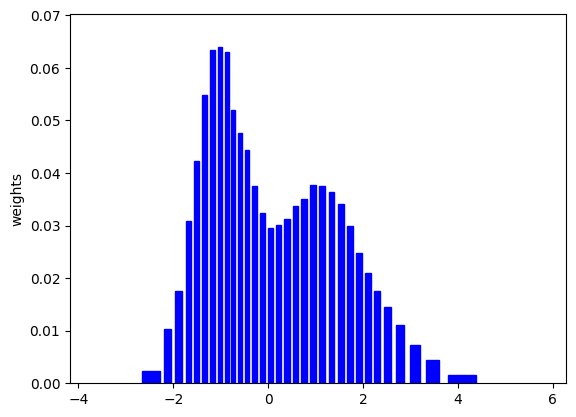
\includegraphics[width=\textwidth]{Figures/fused_analysis.png}
		\end{minipage}
		\hfill
		\begin{minipage}{0.48\textwidth}
			\centering
			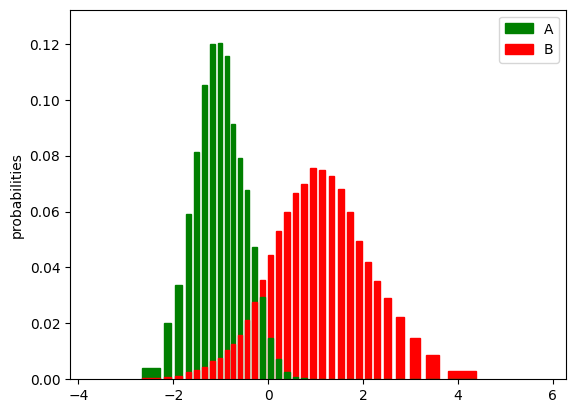
\includegraphics[width=\textwidth]{Figures/separated_analysis.png}
		\end{minipage}
	\end{center}
	\end{modified}

\end{exempli_gratia}

\begin{modified}
	In the example, an intuitive definition of a comparison value between works is proposed using clustering. In such contexts, clustering proves to be an effective tool for handling the complexity and sparsity of high-dimensional data. This is particularly relevant for counteracting the curse of dimensionality, a phenomenon where the volume of the data space is inherently vast compared to the number of available data points. In such scenarios, rigid box-based discretisations often fail because they divide the space into a fixed grid, which becomes inefficient as the dimensionality increases. The result is an exponential increase in the number of boxes, most of which remain empty or sparsely populated, leading to poor generalization.

	\noindent By contrast, dynamic clustering the data with methods such as \gls{kmeans} or \gls{fcm} allows an adaptive representation that aligns with the data distributions. Instead of imposing fixed boundaries, the centroids are positioned to capture meaningful structures in the data, improving both computational efficiency and empirical performance. This flexibility makes dynamic clustering a practical and effective choice for high-dimensional problems.
\end{modified}

\begin{toReview}
\begin{exempli_gratia}[Curse of Dimensionality]
	In this example, we compute the comparison value between the distribution \(\mathcal{N}\left(\vec{0}, \mathds{1}_\texttt{d}\right)\) in \(\mathbb{R}^K\) and itself for different values of \(K\).

	\noindent Specifically, for each \(K\), two samples \(A\) and \(B\), each containing 128 points, are taken from the same distribution. The samples are compared using two approaches: a static clustering approach (box-based) and a dynamic clustering approach (\gls{kmeans}). In the box-based method, the space is divided into \(2^K\) boxes (2 boxes per axis), while in the \gls{kmeans} method, the number of centroids is fixed at \(2\). The table below shows the average comparison values as \(K\) varies:

	\begin{minipage}{\textwidth}
		\centering
		\begin{tabular}{|>{\columncolor{pink}}c|c|c|c|c|c|}
			\hline
			Dimensions & \(1\) & \(2\) & \(4\) & \(8\) & \(16\) \\
			\hline
			Comparison with clustering & \(0.00\) & \(0.00\) & \(0.00\) & \(0.00\) & \(0.00\) \\
			\hline
			Comparison without clustering & \(0.00\) & \(0.01\) & \(0.04\) & \(0.57\) & \(1.00\) \\
			\hline
		\end{tabular}
	\end{minipage}

	\noindent Now consider two sets \(A\) and \(B\) of samples drawn from \(\mathcal{N}(\vec{0}, \mathds{1})\) and \(\mathcal{N}(\vec{1} / \sqrt{K}, \mathds{1})\) in \(\mathbb{R}^K\). These Gaussian distributions are equidistant regardless of the dimensionality \(K\), so we expect stable results. The table below reports the results of this comparison:

	\begin{minipage}{\textwidth}
		\centering
		\begin{tabular}{|>{\columncolor{pink}}c|c|c|c|c|c|}
			\hline
			Dimensions & \(1\) & \(2\) & \(4\) & \(8\) & \(16\) \\
			\hline
			Comparison with clustering & \(0.07\) & \(0.07\) & \(0.05\) & \(0.03\) & \(0.02\) \\
			\hline
			Comparison without clustering & \(0.08\) & \(0.08\) & \(0.11\) & \(0.62\) & \(1.00\) \\
			\hline
		\end{tabular}
	\end{minipage}

	\noindent The number of centroids is a critical parameter. As with boxes, too many centroids can overfit, increasing the comparison value, while too few may fail to capture the data's structure efficiently. Additionally, in high-dimensional spaces, box-based clustering becomes computationally prohibitive compared to dynamic clustering, with computation times exceeding those of \gls{kmeans} by a factor of over 100. The dynamic shape of \gls{kmeans} clusters explains this difference: a single dynamically generated cluster can cover regions spanning thousands of boxes, drastically reducing computational cost while preserving accuracy.
\end{exempli_gratia}
\end{toReview}
\newpage
\subsection{Fuzzy Clustering as a Noise Filtering Method}
\begin{modified}
In this thesis, a variant of the algorithm \gls{fcm} will be used to compare two datasets. This variant introduces a weighting factor $w$, which represents the importance or contribution of each data point in the clustering process. The weight $w$ can be interpreted as the effective cardinality of the point: for instance, a point with $w=2$ is treated as if it were two identical points, while $w=0.5$ corresponds to half a point. This generalization allows for cleaner comparisons between sets of samples with different cardinality, simulating a balanced dataset by appropriately scaling the influence of each point.

\noindent Additionally, this variant includes specific adjustments to account for machine error in the computation of centroids (see \cref{alg:FuzzyClustering}). These adjustments improve robustness in high-dimensional spaces, with large datasets, or when using many centroids, mitigating numerical precision issues for stable clustering.
\end{modified}
\paragraph{Data's weight}
We introduce a vector $w$ indicating the weight of the data as a positive real value. As stated in \cref{thm:Mupdate,thm:Eupdate,def:fuzzyloss}, the following equations summarize the key components of the fuzzy clustering algorithm discussed so far:
\begin{align*}
	c_{j}^\text{new} &= \frac{\sum_{i=1}^N u_{ij}^2x_i}{\sum_{i=1}^N u_{ij}^2w_i} \quad \forall j\\
	L &= \sum_i\sum_j u_{ij}^2\left\|x_i-c_j\right\|^2 \\
	u_{ij} &= \frac{1}{\sum_k\frac{d_{ij}^2}{d_{ik}^2}} \quad \forall i,j\\
	d_{ij} &= \left\|x_i - c_{j}\right\| \quad \forall i,j
\end{align*}
Since it is a weighted average over $u_{ij}^2$, if a datum has a higher weight then it should increase its influence, thus having the following results:
\begin{align*}
	c_{j}^\text{new} &= \frac{\sum_{i=1}^N u_{ij}^2w_ix_i}{\sum_{i=1}^N u_{ij}^2w_i} \quad \forall j\\
	L &= \sum_i\sum_j w_{i}u_{ij}^2\left\|x_i-c_j\right\|^2 \\
	u_{ij} &= \frac{1}{\sum_k\frac{d_{ij}^2}{d_{ik}^2}} \quad \forall i,j\\
	d_{ij} &= \left\|x_i - c_{j}\right\| \quad \forall i,j
\end{align*}

\paragraph{machine error}
The use of \gls{fcm} in this thesis involves millions of data, and it is possible that the classical algorithm will find itself making serious machine errors that must be kept under control. In \cref{alg:FuzzyClustering}, might exist is a value $D_{ik}^2 \approx 0$  that may be null or so small that when $D_{ij}^2 / D_{ik}^2$ is computed, it is infinity or a number so large that when added to other numbers it overshadows all other data in the sum.\\ For this reason \cref{alg:MembershipUpdateSafe} proposes a more robust approach. We also remark that the computational cost in a sequential algorithm will be $O(NMK)$. However scalability allows us to reduce this cost to $O(\text{log}(KM))$ by exploiting the independence of each cycle and scalable reductions (details in \cref{chap:methodology}).\\

\begin{algorithm}[h]
\caption[Membership update stable computation.]{Membership update stable computation.\\
	\begin{minipage}[t]{\linewidth}
		\textsc{INPUT}
		\begin{itemize}[noitemsep, topsep=0pt]
			\item[$\mathcal{S}$:] set of data $x_1,\dots,x_N$
			\item[$\mathcal{C}$:] centroids $c_1,\dots,c_M$
		\end{itemize}
	\end{minipage}
}
\begin{algorithmic}[1]
\Procedure{MembershipUpdateStable}{$\mathcal{S}, \mathcal{C}$}
    \State $D^2 \gets (d^2_{ij})_{ij}$ with $d_{ij}^2=\|x_i-c_j\|^2$
    \For{$i \gets 0$ to $N$}
        \State $l \gets \min_k\{D_{ik}^2\}$
        \If{$l = 0$}
            \Where{$D_{ij}^2=0$}{$u_{ij}\gets1$}
            \Where{$D_{ij}^2\neq0$}{$u_{ij}\gets0$}
        \Else
            \State $u_{ij} \gets \frac{l}{D_{ij}^2}\quad \forall j$
        \EndIf
        \State $S_i \gets \sum_j u_{ij}$
        \State $u_{ij} \gets u_{ij} / S_i\quad\forall j$
    \EndFor
\EndProcedure
\end{algorithmic}
\label{alg:MembershipUpdateSafe}
\end{algorithm}

\subsection{Analysis of images with DFT}
It was seen in the introductory section of \gls{dft} that the algorithm \gls{fft} can only be applied to time series or, more generally, to a sequence of complex numbers. However, it is also possible to extend this concept to the analysis of the spectrum of a matrix with periodic behaviour.

\noindent Consider a matrix $x \in \mathbb{C}^{N \times M}$ defined as follows:
\[
x_{n,m} = \cos\left(\omega_rn+\omega_cm\right)
\]
It can be shown that its \gls{dft} results in a matrix of the same shape as $x$, where the only nonzero component is in the row corresponding to $\omega_r$ and in the column corresponding to $\omega_c$.

\noindent This is analogous to the application of \gls{cft} on $\mathbb{R}^2$. In particular, we would like to obtain the following inverse relation to reconstruct $x$ from its Fourier coefficients:
\begin{equation}
	x_{n,m} = \frac{1}{NM}\sum_{r,c} X_{r,c} e^{i2\pi\left(\frac{rn}{N} + \frac{cm}{M}\right)}
\end{equation}
Where the Fourier coefficients $X_{r,c}$ are given by:
\begin{equation}
	X_{r,c} = \sum_{n,m} x_{n,m}e^{-i2\pi\left(\frac{nr}{N} + \frac{mc}{M}\right)}
\end{equation}
At the algorithmic level, the two-dimensional \gls{fft} is obtained by applying the algorithm to the columns first and to the rows of the original matrix $x$. In particular:
\begin{align*}
	y_{r,m} &= \sum_{n} x_{n,m}e^{-i2\pi\frac{nr}{N}} & \;\;\text{over each column apply \gls{fft}}\\
	X_{r,c} &=\sum_{m}y_{r,m}e^{-i2\pi\frac{mc}{M}} & \;\;\text{over each row apply \gls{fft}}
\end{align*}
\begin{exempli_gratia}
	We analyse a matrix composed of several overlapping frequencies and Gaussian noise with variance $1$.
	\begin{align*}
	x_{n,m} &= 2\cos\left(2\pi(2n + 3m) + 3\right) \\
	&+ 0.8\cos\left(2\pi(n + 5m) + 2\right) \\
	&+ \cos\left(2\pi(7n + 5m)\right) + \mathcal{N}_{n,m}
	\end{align*}
	\begin{modified}
		In the figure, the original data is shown on the left as a 2D matrix visualized using the \texttt{viridis} color scale, while the Fourier coefficients computed from this matrix are displayed on the right.
	\end{modified}
	\begin{center}
		\centering 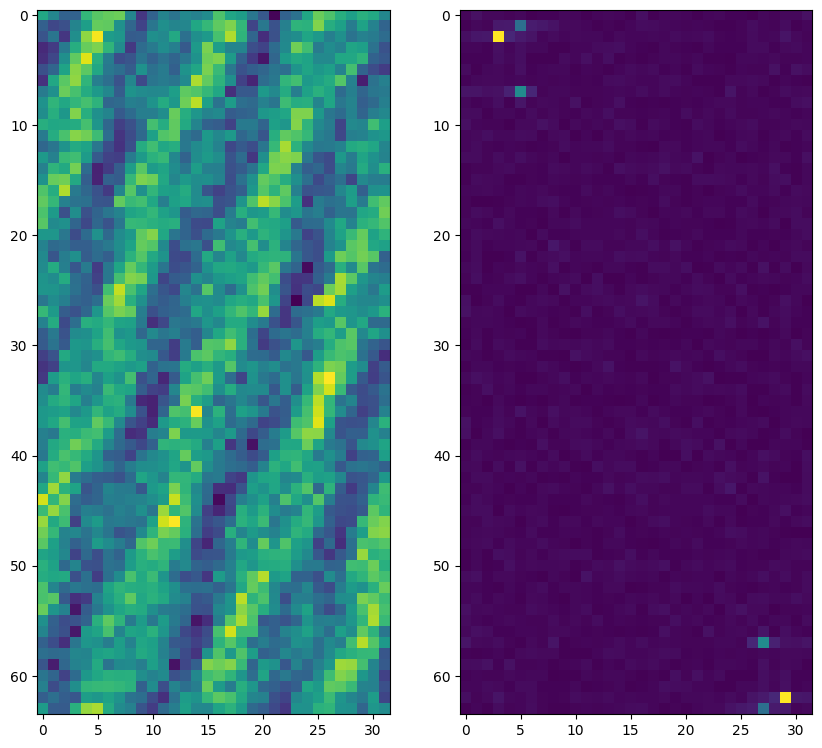
\includegraphics[width=0.6\textwidth]{Figures/fft2d_example.png}
	\end{center}
\end{exempli_gratia}

\noindent The two-dimensional \gls{fft} can be used to analyse periodic patterns in matrices that represent images or signals. Typical applications include filtering, image compression and pattern recognition, where the spectral decomposition allows significant components to be distinguished from the noise.
  % Revisione della bibliografia
\chapter{Methodology}
\label{chap:methodology}
%Questa ricerca si propone di analizzare l'attribuzione di opere grafiche, prendendo spunto dalle metodologie utilizzate per l'attribuzione di opere letterarie. In particolare, si esamina l'applicazione degli $N$-grammi, ossia sequenze di $N$ simboli adiacenti, come metodo di rappresentazione delle opere.
This research aims to analyse the attribution of graphic works, taking its inspiration from the methodologies used for the attribution of literary works \citep[see][]{thesis}. In particular, it examines the application of $N$-grams, i.e. sequences of $N$ adjacent symbols, as a method of representing works.

%\noindent Per comprendere appieno la rappresentazione delle opere pittoriche, è opportuno partire dal metodo utilizzato per le opere letterarie. Ad esempio, nell'espressione "\texttt{Hello world!}", un $3$-gramma può essere rappresentato da "\texttt{llo}", che corrisponde a una sequenza di $3$ caratteri consecutivi. È importante sottolineare che anche spazi e punteggiature sono considerati caratteri, quindi anche "\texttt{o w}" e "\texttt{ld!}" sono $3$-grammi validi.
\noindent To fully understand the representation of graphic works, it is appropriate to start from the method used for literary works. For example, in the expression "\texttt{Hello world!}", a $3$-gram can be represented by "\texttt{llo}", which corresponds to a sequence of $3$ consecutive characters. Importantly, spaces and punctuation are also considered characters, so "\texttt{o w}" and "\texttt{ld!}" are also valid $3$-grams.

%\noindent Le ricerche in questo ambito sono numerose e hanno portato a diverse applicazioni. Le rappresentazioni basate sugli $N$-grammi sono utilizzate non solo nell'attribuzione letteraria, ma anche nei modelli di linguaggio naturale nei quali queste analisi sono integrate con uso di reti neurali ricorrenti \begin{toDo} Inserire un riferimento \end{toDo}. Tuttavia, finora si conosce poco riguardo all'applicazione di questa tecnica alle opere pittoriche, e questo costituisce l'obiettivo principale della presente ricerca.
\noindent Research in this field is extensive and has led to various applications. Representations based on $N$-grams are used not only in literary attribution, but also in natural language models in which these analyses are integrated with the use of recurrent neural networks. However, little is known so far about the application of this technique to graphic works, and this constitutes the main focus of this research.

% introduco la tesi della triennale
\paragraph{\gls{dada}}
In the thesis research about the application of $N$-gram analysis on calligraphic works, \citep[see][]{thesis}, a graphic work is considered as matrix of pixels and an $N$-gram was defined as a square sub-matrix of size $N$, also called 'tile'.

\noindent The research focused on the analysis of images that have been reduced to matrices, in which the only colours present are black and white (see \cref{fig:example_bw}). This process, known as 'posterisation', aims to reduce the amount of colours present in the work (known as 'depth'). This methodological choice was motivated by the need to manage the size of the alphabet; indeed, while in a literary work there may exist up to $32^N$ distinct $N$-grams (considering the $26$ letters of the alphabet plus $6$ punctuation symbols), in a pictorial work there may be $256^{3N^2}$ distinct tiles with side $N$. This considerable difference caused significant challenges in image analysis, rendering the application of tools designed for literary works on graphic works ineffective.

\begin{figure}[ht]
	\centering
	\begin{subfigure}{0.4\linewidth}
		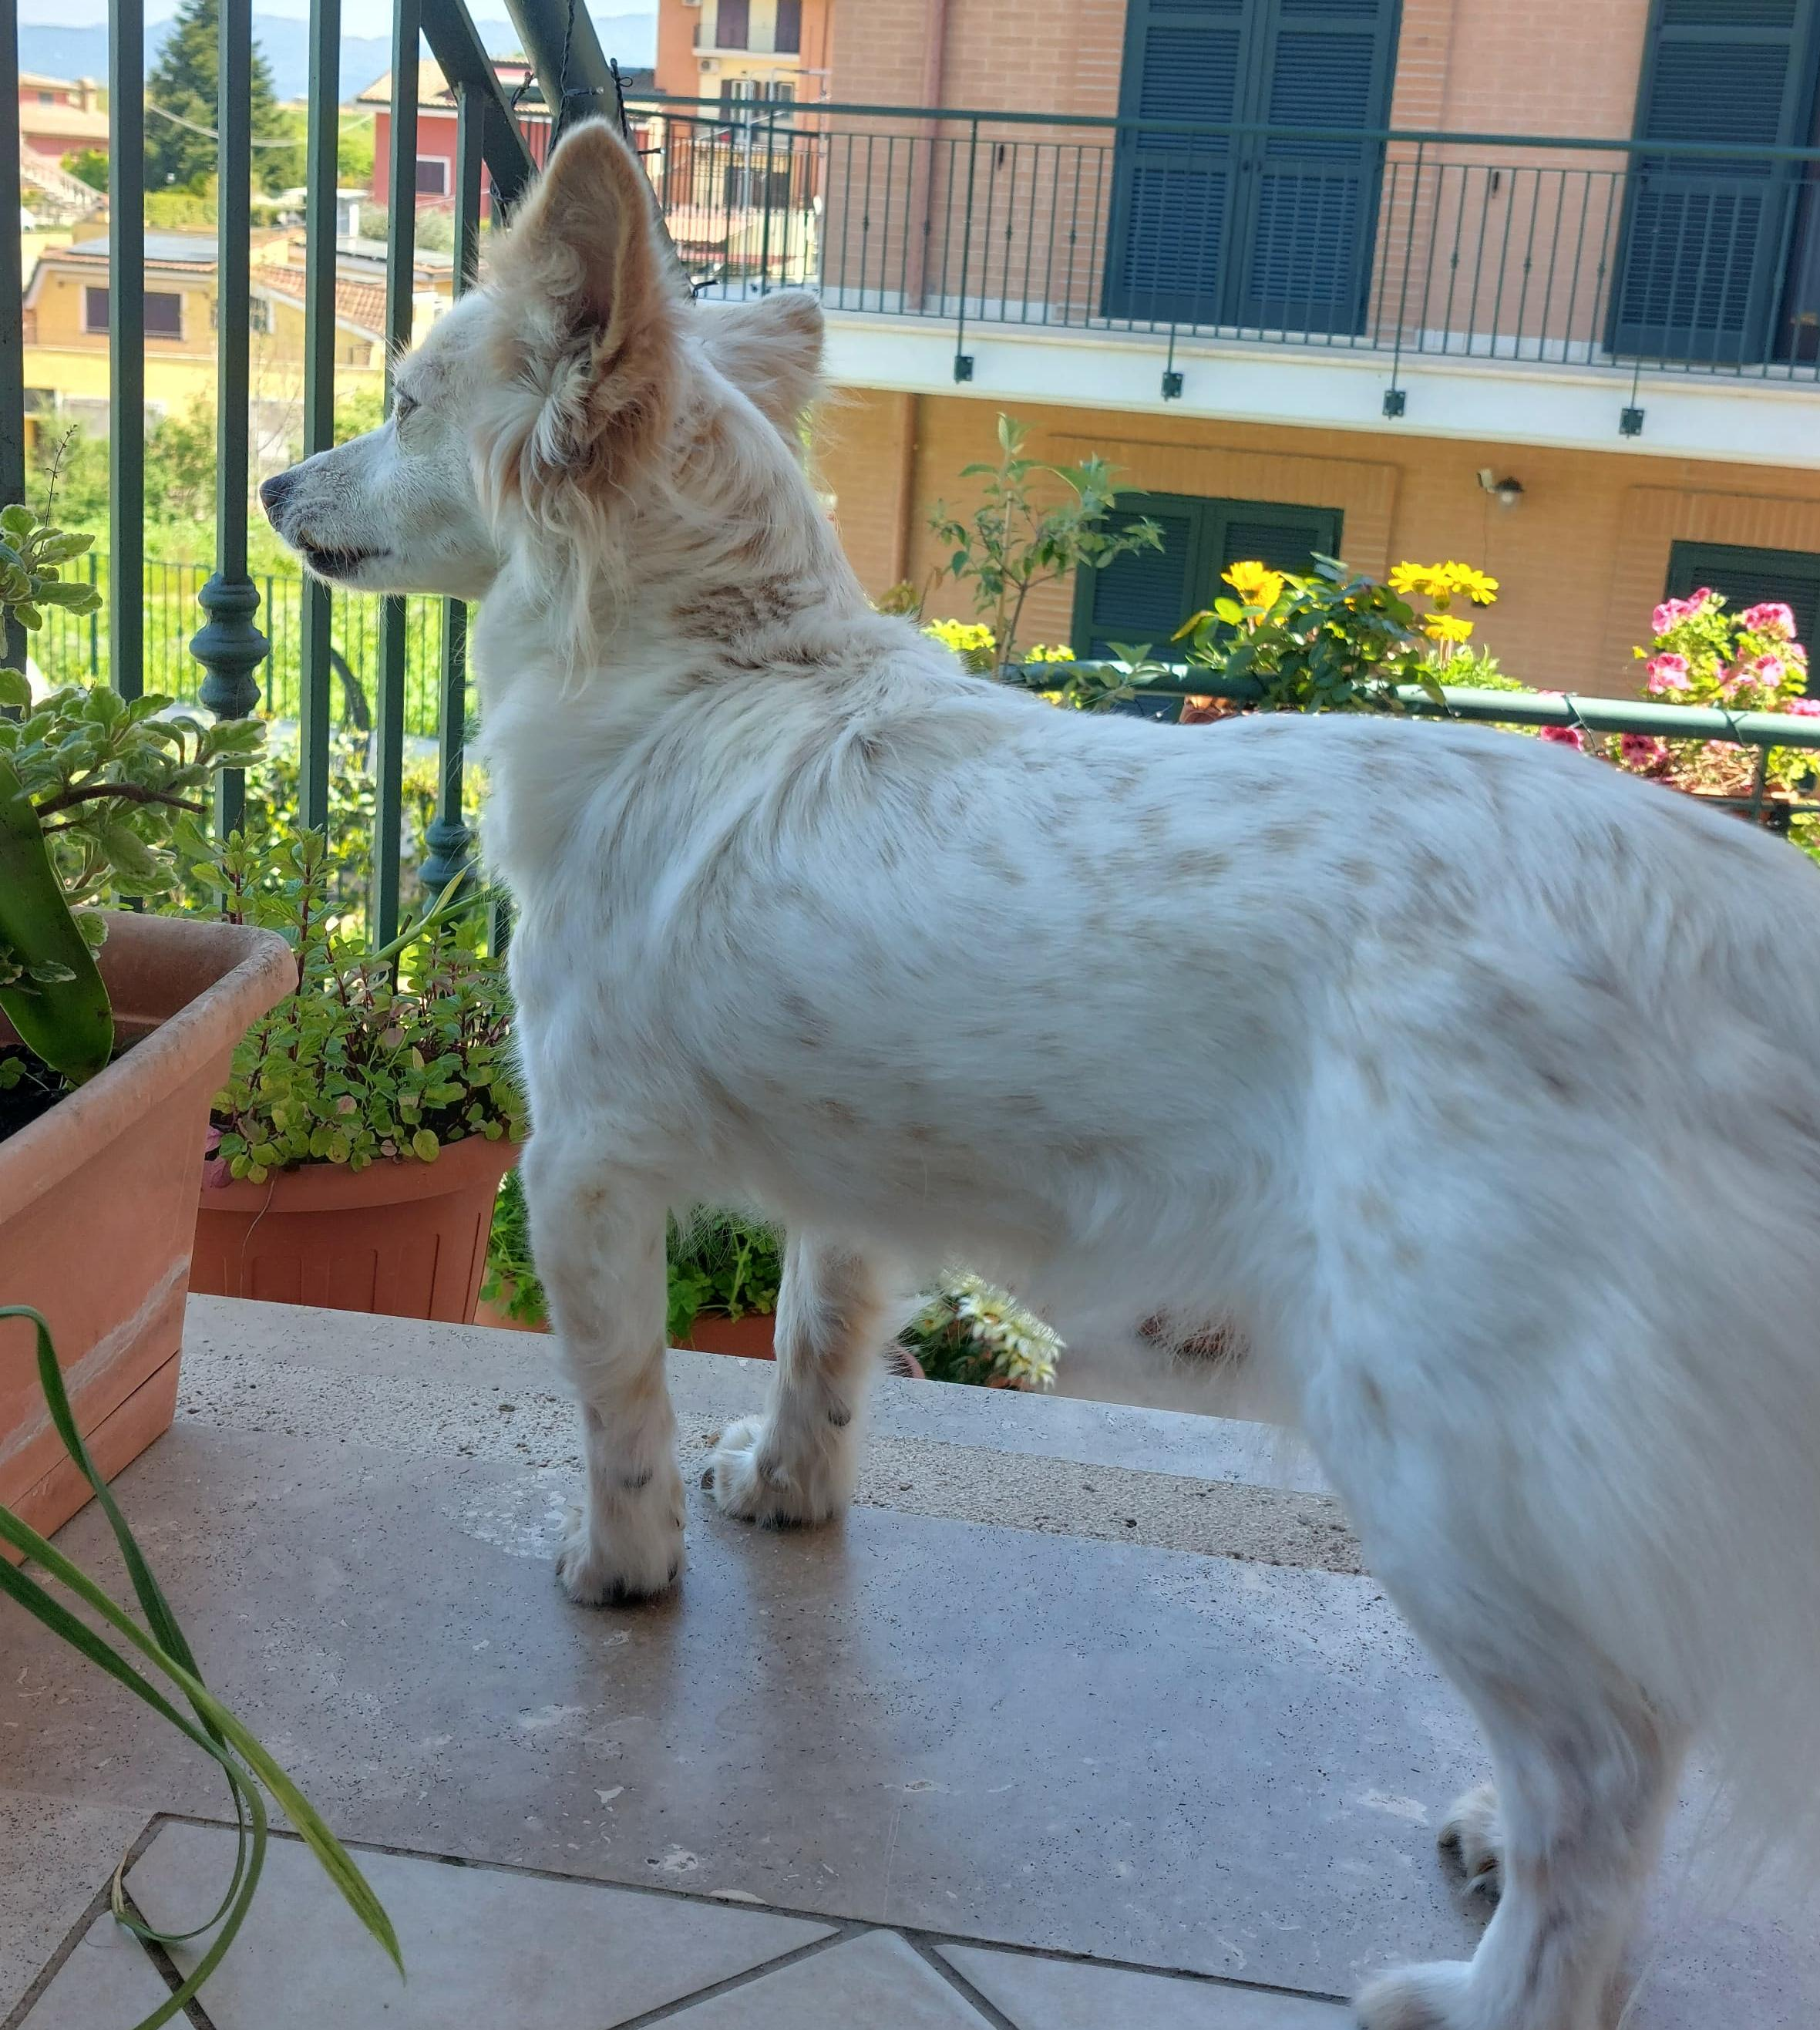
\includegraphics[width=\linewidth]{Figures/example.jpeg}
	\end{subfigure}
	\hspace{2cm}
	\begin{subfigure}{0.4\linewidth}
		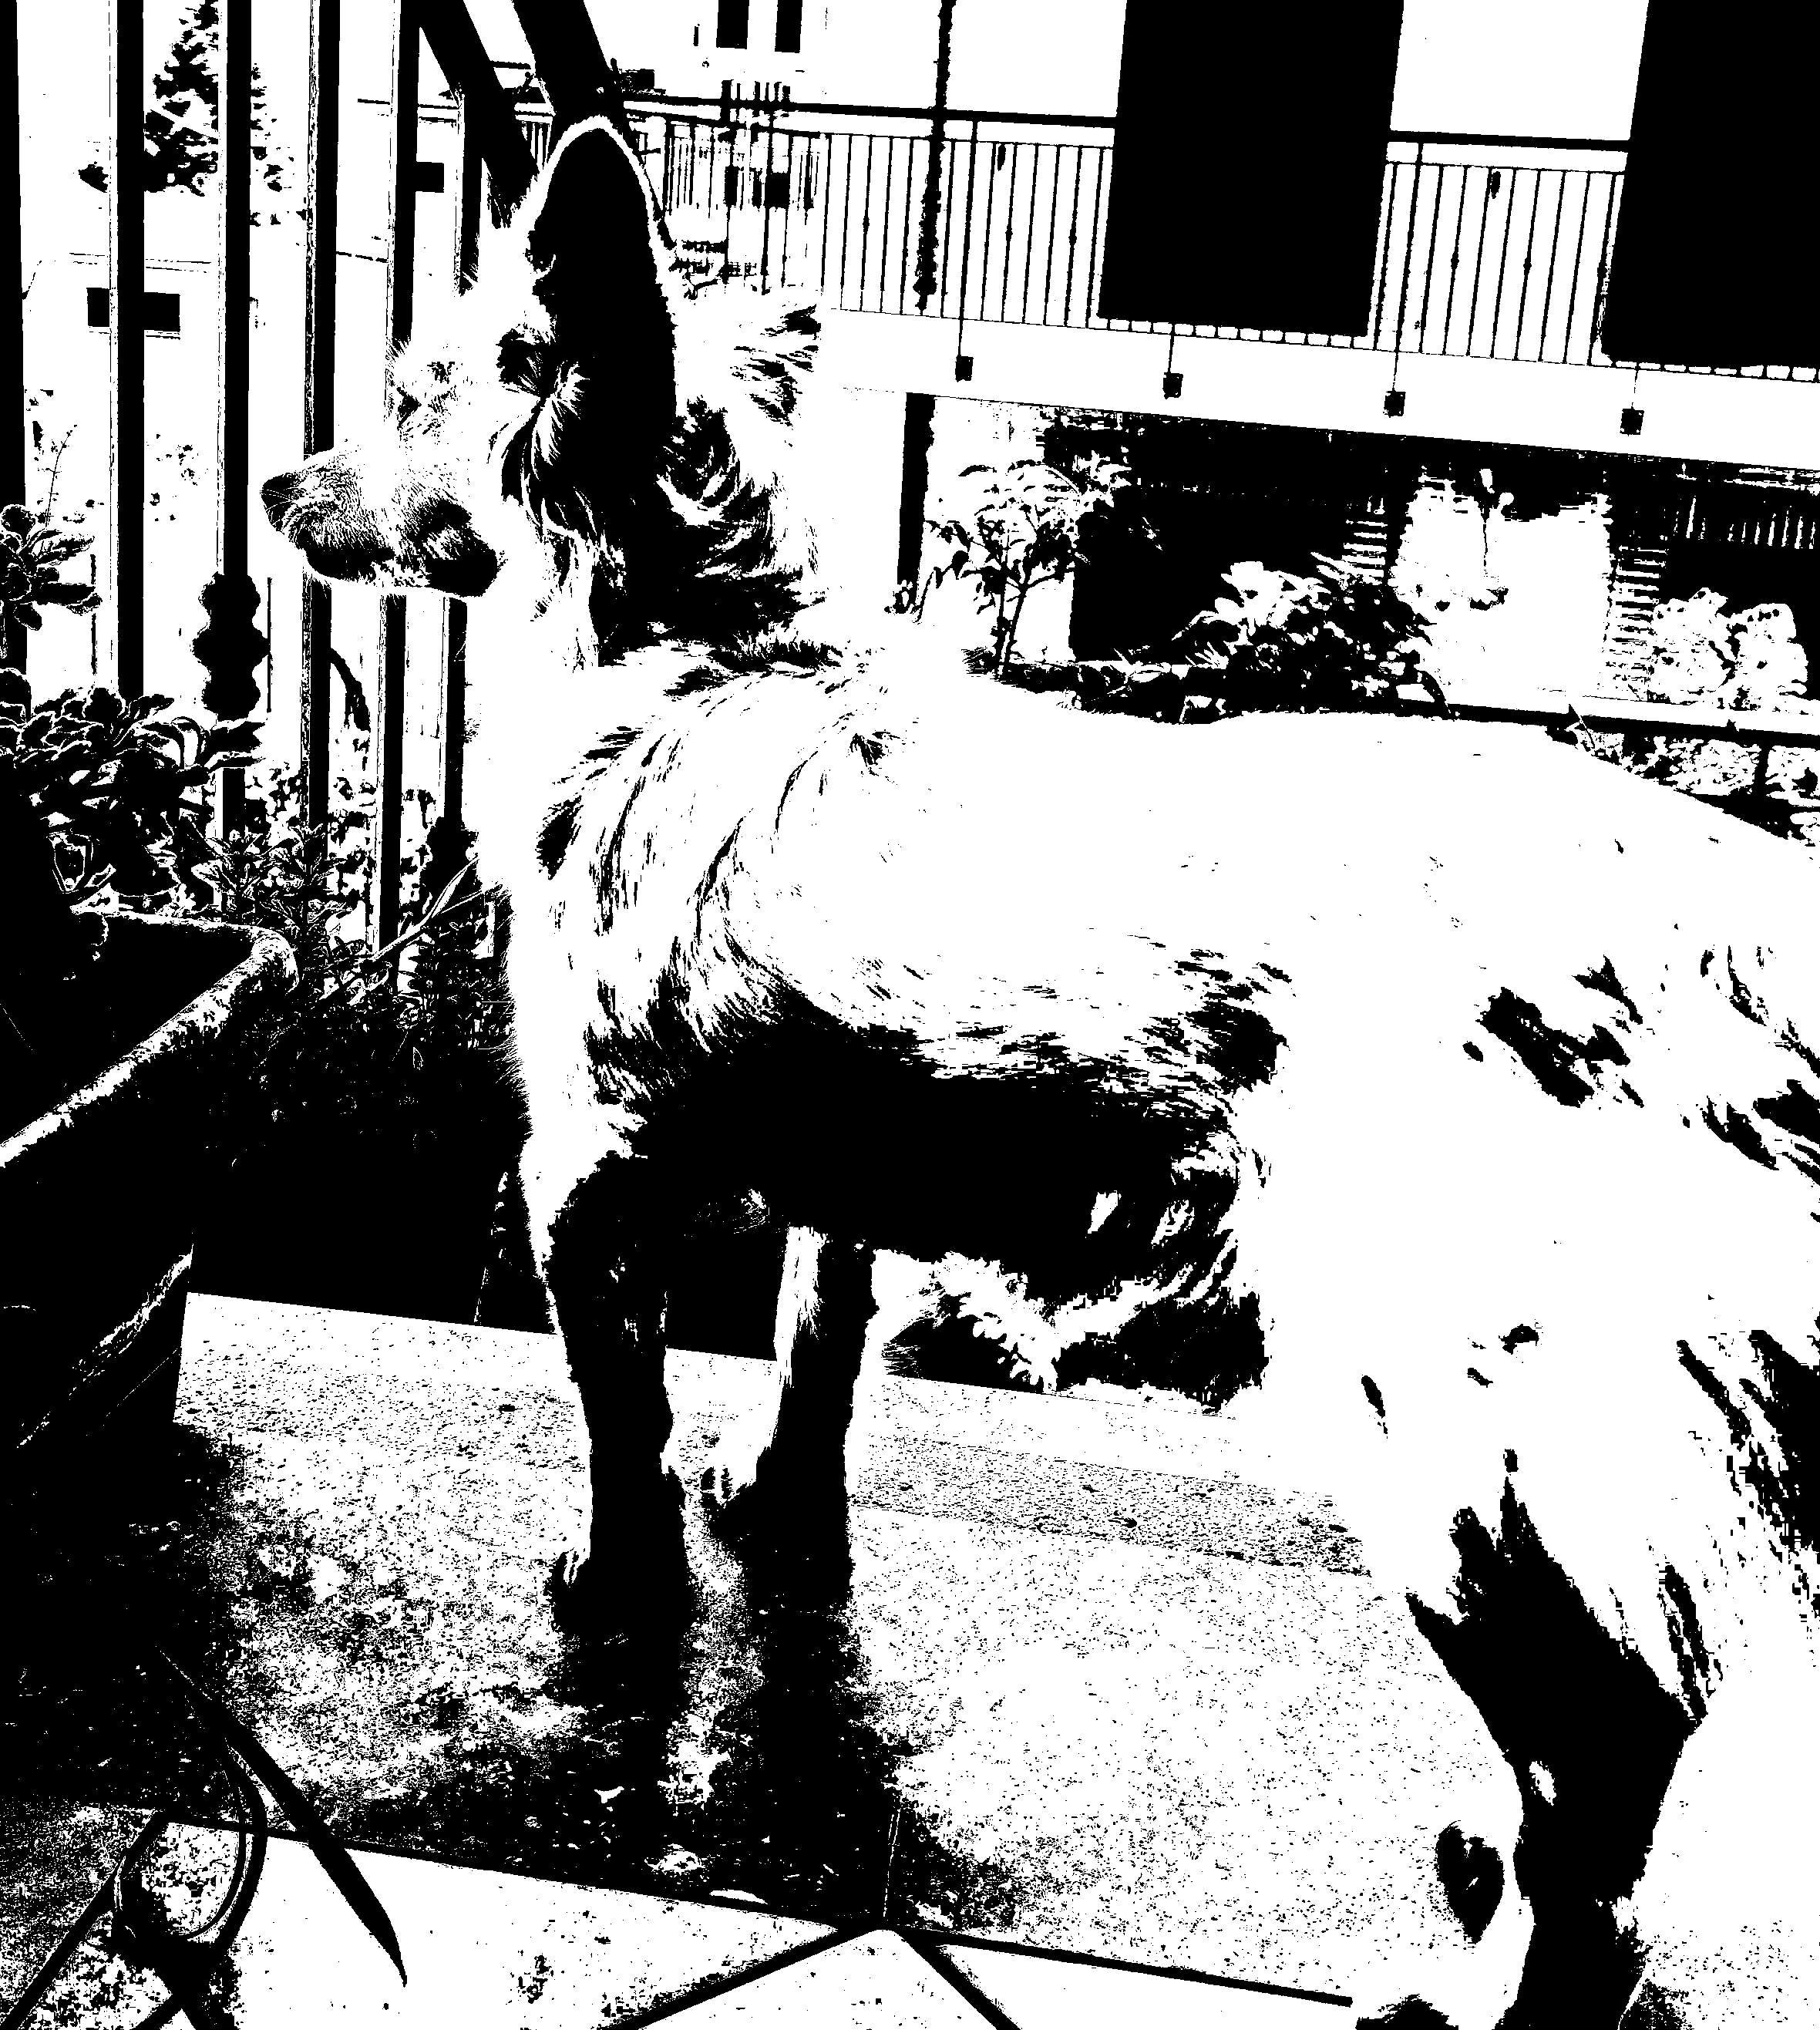
\includegraphics[width=\linewidth]{Figures/example_bw.jpeg}
	\end{subfigure}
	\caption[BW transformation]{Example of a conversion from a coloured image to an image with only black and white (bw) pixels. The image is transformed to greyscale by reducing the saturation, finally half of the lightest pixels are rendered white and the remaining are rendered black.}
	\label{fig:example_bw}
\end{figure}

\noindent The research concluded with promising results, showing that the automatic analysis of handwriting samples allows very precise author attributions. However, it turned out that applying the same analysis to pictorial works such as panels and drawings does not produce satisfactory results. It was conjectured that this is due to the intrinsic nature of pictorial works, where the presence of colour plays an important role, and posterisation, instead of helping attribution, generates noise and new information that make the representation of data unreliable.

\begin{note} in questo paragrafo vorrei solo introdurre il concetto di \gls{dada}, potrei parlare di più della tesi triennale in literature review. \end{note}

\paragraph{\gls{cada}}
%Seguendo la stessa linea di ricerca della tesi di \begin{toDo} inserire riferimento \end{toDo}, abbiamo proposto un riadattamento della metodologia al fine di indagare su quale possa essere la strategia più efficace per l'analisi automatica di immagini caratterizzate da un vasto alfabeto di colori. L'obiettivo è costruire una \gls{cada} che possa analizzare i colori nel loro spazio naturale, ovvero in uno spazio continuo. Ciò ci consentirà di superare il vincolo del discreto di \gls{dada} e di ottenere risultati più accurati e dettagliati.
Following the same line of research \cite[my bachelor thesis]{thesis}, we have proposed a re-adaptation of the methodology in order to investigate what might be the most effective strategy for the automatic analysis of images characterised by a large alphabet of colours. The aim is to construct a \gls{cada} that can analyse colours in their natural space, i.e. in a continuous space. This will allow us to overcome the discrete constraint of \gls{dada} and obtain more accurate and detailed results.

\begin{note} lavoro in scale di grigi, ma è comunque uno spazio continuo \end{note}

\noindent Image analysis in \gls{dada} is a process in five stages: acquisition, pre-processing, synthesis, comparison and attribution. In this paper we are going to focus on the first four phases, detailing the process up to image comparison, while attribution will be briefly discussed as the concluding phase.

\noindent The acquisition phase digitises two-dimensional works of art by scanning or photography. Scanning, in particular, allows a high resolution and accurate representation of the original document, while photography allows greater flexibility when the size of the work or physical conditions make scanning complex. The result of this phase is a digital image that accurately represents the work to be analysed.

\noindent The pre-processing phase prepares the image for analysis by removing irrelevant elements through pixel-wise and work-size transformations. Pixel-wise techniques, such as greyscale conversion, act on each individual pixel. Work-size transformations, on the other hand, act on the image as a whole, e.g. with compression techniques or normalisation of colour scales.

\noindent The synthesis phase deconstructs the image into a list of tiles of size $N\times N$, generating a sequence of discrete elements representing portions of the image. This process, aligned with the idea of n-gram language models, allows stylistic features to be analysed in a $\mathbb{R}^{N^2}$ space, preparing the data format for later comparison.

\noindent In the comparison phase, we are going to address the real computational and theoretical challenge. Clustering techniques will be used to dynamically discretise the space of tiles and organise them according to similarity criteria. This allows us both to efficiently process the large number of tiles in a very high dimension and also to compare the target work with known works in the database.

\noindent Finally, in the attribution phase, the similarities between the target work and known works are examined. The aim is to identify the author of the target work by studying the closest works in terms of stylistic and compositional characteristics. This phase focuses on identifying the works that show the greatest stylistic affinity with the target work, suggesting possible attributions.

%(aggiunto direttamente in inglese)
\noindent This research not only aims to tackle technical and computational challenges, but also to explore new perspectives in the analysis of artworks, thus opening up new horizons in the field of art criticism and art attribution.

% acquisition and dataset details
\section{Data Set}
\subsection{Description}
In this study, the data set consists of a set of graphic works for which attribution is established and unambiguous and for which a uniform resolution expressed in \gls{dpi} is known. It was decided to use calligraphic works, as evidenced in \cite{thesis}. The use of calligraphic works represents a promising first way for artistic attribution.

\noindent The dataset used in the reference article consisted of authentic and unaltered handwriting samples. In this study, the dataset consists of university notes, which do not have a sufficiently high standard and therefore present some significant challenges:

\begin{itemize}
\item \textbf{The squares}: Note sheets often contain small squares that could be mistaken for the author's handwriting. This visual interference can complicate the attribution process.
\item \textbf{Use a variety of writing tools}: University notes can be written using a variety of writing tools, such as highlighters, markers, pencils or white-out. These different writing tools produce different lines and colours, which can affect the attribution of authorship.
\item \textbf{Different graphical contexts}: Notes can contain a variety of elements such as mathematical formulae, graphs and erasures. These features represent heterogeneous graphical contexts that add complexity to the analysis.
\item \textbf{Scanning contamination}: The quality of the page scan can introduce blemishes into the record. These blemishes, such as stains or blurring, can affect the clarity and legibility of the works.
\end{itemize}

\noindent In addition, the use of a pen with a thickness of $0.4\operatorname{\mathrm{mm}}$ on the sheet was considered a reasonable first choice since in \cite{thesis} the stroke had the same thickness. This particular aspect is also important in ensuring a certain uniformity and consistency in the visual attributes of the works under examination, thus facilitating a more accurate attribution of authorship.

\noindent The dataset is organised into $4$ authors, and the included images are as follows:

\begin{itemize}
\item The images are saved in the \gls{png} format.
\item Each image is composed of three colour channels \gls{rgb}, each with a depth of 8 bits.
\item The original sheets were scanned at a resolution of 400 \gls{dpi}.
\item The thickness of the pen used to write on the original sheets is $0.4\operatorname{\mathrm{mm}}$.
\end{itemize}

\noindent The images were then cut to remove large impurities or large white spaces. Finally leaving a total of $420$ images.

\begin{table}[h]
    \centering
    \begin{tabular}{|>{\columncolor{pink}}c|c|c|c|}
        \hline
        \rowcolor{lavender}
        \cellcolor{mint} AuthorID & Num of items & Size & Mean side length \\
		\hline
        $1$ & $270$ & $554\operatorname{\mathrm{MB}}$ & $\num{1.43}\operatorname{\mathrm{Kpx}}$ \\
        \hline
        $2$ & $43$ & $133\operatorname{\mathrm{MB}}$ & $\num{1.8}\operatorname{\mathrm{Kpx}}$ \\
        \hline
        $3$ & $56$ & $227\operatorname{\mathrm{MB}}$ & $\num{2.0}\operatorname{\mathrm{Kpx}}$ \\
        \hline
        $4$ & $51$ & $247\operatorname{\mathrm{MB}}$ & $\num{2.2}\operatorname{\mathrm{Kpx}}$ \\
        \hline
        \hline
        \cellcolor{mint} Total & $420$ & $1.2\operatorname{\mathrm{GB}}$ & $\num{1.7}\operatorname{\mathrm{Kpx}}$ \\
        \hline
    \end{tabular}
    \caption[Summary of dataset]{Each item is a cleaned area of the original images. The size represent the total number of pixels. The last column is the geometric mean of the side length, it's compute as follow: $\sqrt{\frac{\text{Num of pixels}}{\text{Num of items}}}$}
\end{table}

In the dataset creation, full clipboard images were collected and then cut to exclude non-pen strokes, highlights, and erasures. In addition, some cuts are particularly small and in a few cases are slightly overlapping.

\begin{figure}[h]
    \centering
    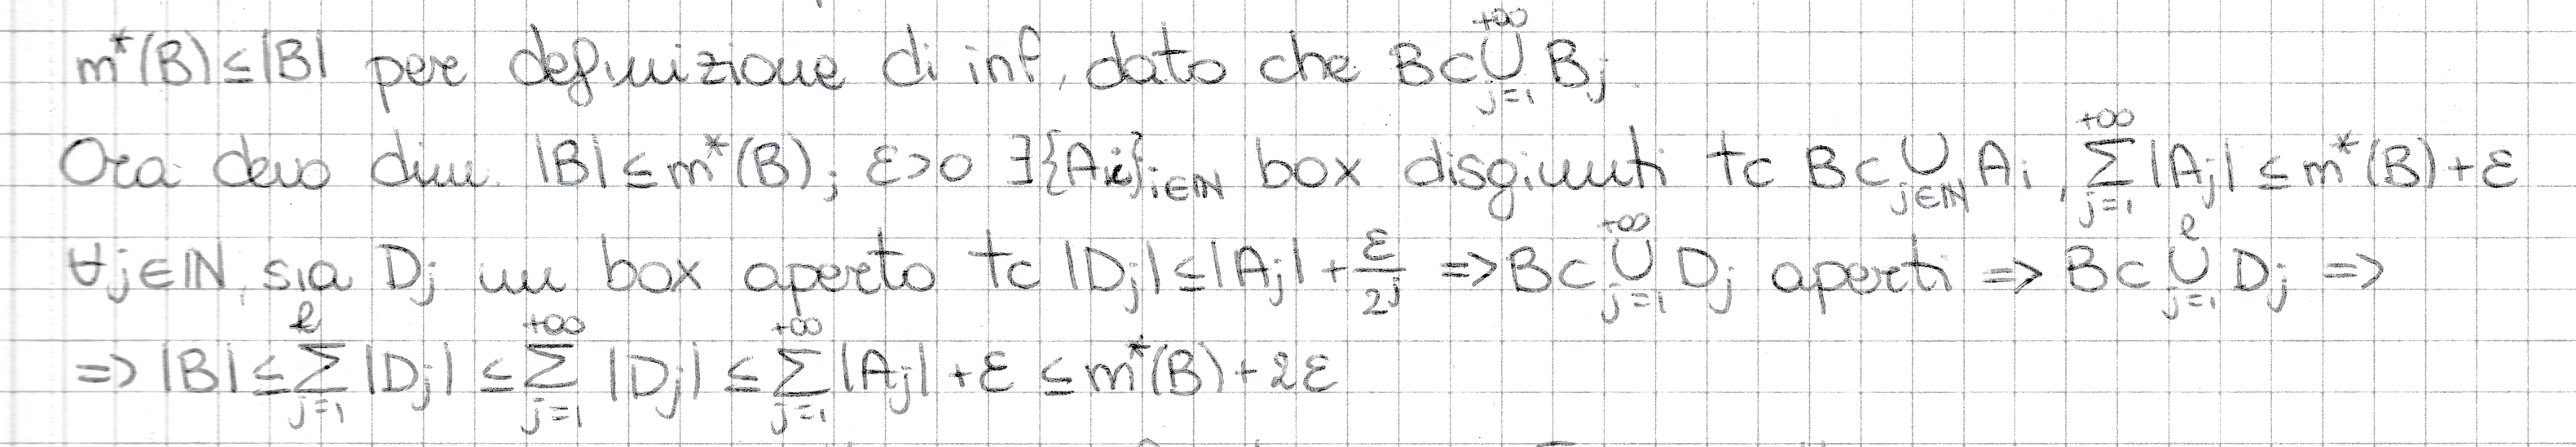
\includegraphics[width=\linewidth]{Figures/Author1_0001_02.png}
\end{figure}


% pre-processing and digitisation theory
\section{Pre processing}
\begin{figure}[ht]
    \centering
    \begin{subfigure}{0.4\linewidth}
        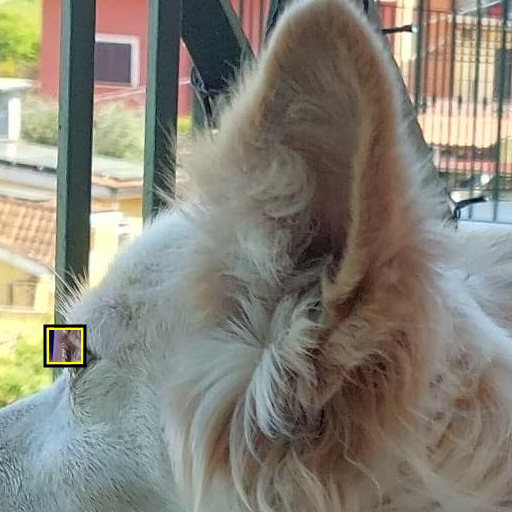
\includegraphics[width=\linewidth]{Figures/example_square.png}
    \end{subfigure}
    \hspace{2cm}
    \begin{subfigure}{0.4\linewidth}
        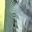
\includegraphics[width=\linewidth]{Figures/example_detail.png}
    \end{subfigure}
    \caption[Pixel grid detail]{Image detail.}
    \label{fig:example_detail}
\end{figure}

%La digitalizzazione delle immagini è un passo fondamentale per preparare le opere d'arte alle analisi che verranno effettuate. Per comprendere appieno il funzionamento di queste trasformazioni, è importante acquisire una conoscenza approfondita del processo attraverso cui un'opera pittorica viene catturata da una macchina fotografica e successivamente digitalizzata in un dispositivo elettronico.
Digitising images is a fundamental step in preparing the data set for analysis. To fully understand how these transformations work, it is important to understand the process by which a work of art is captured by a camera and then digitised in an electronic device.

\paragraph{Definition of image: from the real world to the virtual world}
%Gli artisti dell'antichità utilizzavano varie tecniche, come la camera oscura e i principi della geometria proiettiva, per rappresentare i paesaggi in modo realistico. Durante il Rinascimento, hanno ulteriormente perfezionato questi metodi con strumenti come la camera lucida, mostrando una comprensione matematica avanzata in opere d'arte come la Scuola di Atene di Raffaello.\begin{toDo} citare fonte \end{toDo}.
Artists of antiquity used various techniques, such as the camera obscura and the principles of projective geometry, to represent landscapes realistically. During the Renaissance, they further refined these methods with tools such as the camera lucida, showing advanced mathematical understanding in works of art such as Raphael's School of Athens.\footnote{for more about camera obscura, see\newline\url{https://en.wikipedia.org/wiki/Camera_obscura}}

%\noindent L'invenzione della fotografia nel $1826$, in concomitanza con il movimento artistico del Realismo, segnò un momento fondamentale nella storia dell'arte visiva. La fotografia, con la sua capacità di rappresentare la realtà in modo oggettivo, divenne uno strumento sempre più utilizzato dagli artisti. L'avanzamento delle conoscenze in ottica e chimica portò alla creazione della fotografia analogica \begin{toDo} citare fonte e inserire immagine \end{toDo}.
\noindent The invention of photography in $1826$, in conjunction with the art movement of Realism, marked a fundamental moment in the history of visual art. Photography, with its ability to represent reality objectively, became a tool increasingly used by artists. The advancement of knowledge in optics and chemistry led to the creation of analogue photography.\footnote{for more about history of photography, see\newline\url{https://en.wikipedia.org/wiki/History_of_photography}}
\begin{figure}[ht]
    \centering
    \begin{subfigure}[t]{0.4\linewidth}
        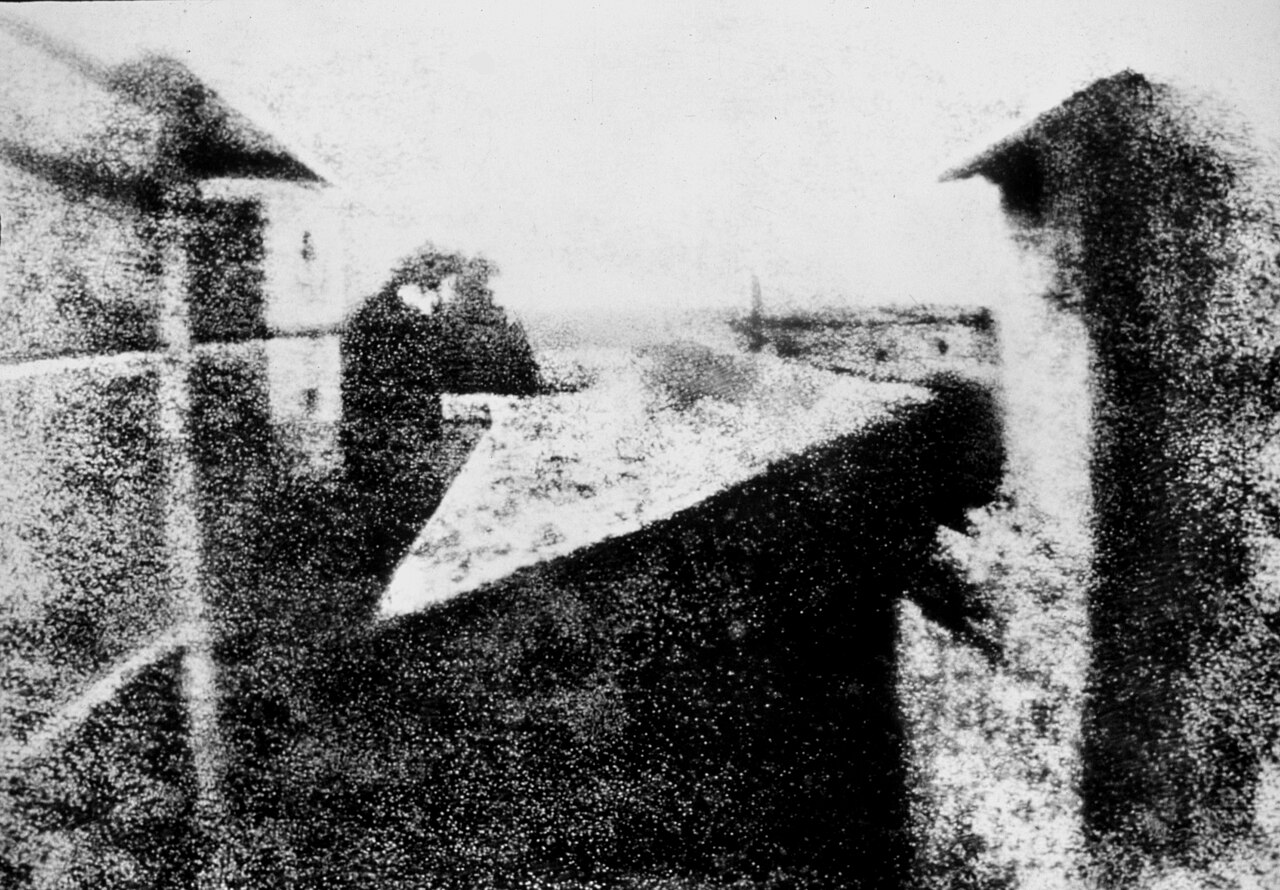
\includegraphics[width=\linewidth]{Figures/FotoStoria.jpg}
        \caption{'View from the Window at Le Gras', Joseph Nicéphore Niépce, c.1826, Heliography, Harry Ransom Center, University of Texas at Austin, USA\cite{FirstPhoto}.}
    \end{subfigure}
    \hspace{2cm}
    \begin{subfigure}[t]{0.4\linewidth}
        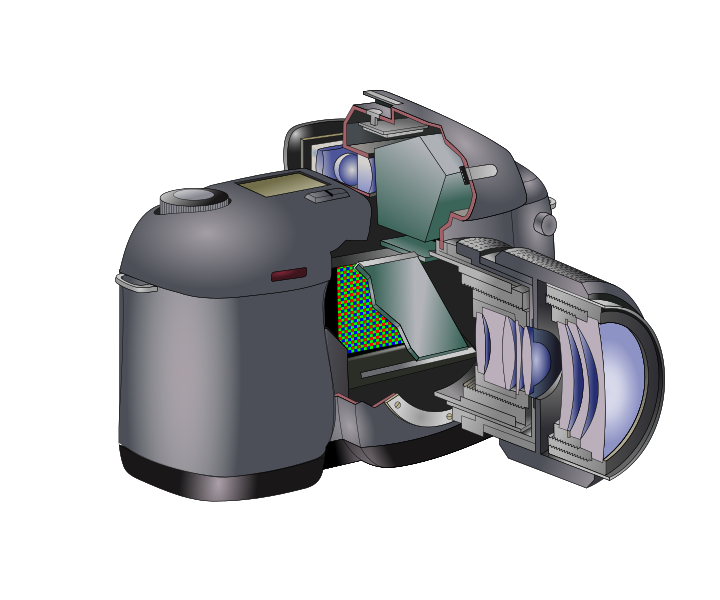
\includegraphics[width=\linewidth]{Figures/digitalcamera.png}
        \caption{Illustration of digital camera\cite{Reflex}.}
    \end{subfigure}
\end{figure}

%\noindent Nel corso degli anni ottanta, con l'avvento della tecnologia informatica, la fotografia digitale divenne una realtà. Il funzionamento di base rimase simile alle tecniche precedenti, ma con l'aggiunta di un nuovo processo di digitalizzazione. Invece di essere impressa su una superficie fotosensibile, l'immagine viene catturata da una griglia di sensori ottici e digitalizzata come una matrice di colori, con ogni componente chiamata "pixel" \begin{toDo} inserire fonte e immagine \end{toDo}.
\noindent During the 1980s, with the advent of computer technology, digital photography became a reality. The basic operation remained similar to previous techniques: instead of being printed on a photosensitive surface, the image was captured by a grid of optical sensors and digitised as a matrix of colours, with each component called a pixel.

%\noindent Il concetto di riproduzione dei colori non è nuovo, e già nel $1855$ James Clerk Maxwell lavorò su questo tema, introducendo il modello di colore \gls{rgb}, ancora oggi ampiamente utilizzato. Questo modello codifica ogni colore con tre numeri reali in un intervallo tra $0$ e $1$. Tuttavia, per scopi informatici, si è convenuto di rappresentare i $3$ valori di un colore con numeri interi compresi tra $0$ e $255$ \begin{toDo} inserire fonte per lavoro di Maxwell \end{toDo}. In questo modo, un'immagine digitale diventa una matrice di triple, rappresentando i valori dei pixel nei tre canali di colore \gls{rgb}.
\noindent The concept of colour reproduction is not new and as early as $1855$ James Clerk Maxwell worked on this subject, introducing the colour model \gls{rgb}, which is still widely used today (see \cite{MaxWell_Colours}). This model encodes each colour with three real numbers in an interval between $0$ and $1$. However, for computing purposes, it was agreed to represent the $3$ values of a colour with integers between $0$ and $255$. In this way, a digital image becomes a matrix of triples, representing the pixel values the three colour channels \gls{rgb}.

\subsection{Grayscale reduction}
The quantisation of colours is expressed in $3$ channels \gls{rgb}, each with an integer value between $0$ and $255$. The choice of these $3$ colours is not arbitrary; it derives from a physiological feature of human vision. Our perception of colour is determined by photoreceptor cells in the eye called cones, of which there are three types: S-cones, M-cones and L-cones. These cones are sensitive to wavelengths that approximately correspond to blue, green and red light respectively.

\noindent This model of colour representation is therefore deeply rooted in the way our visual system works, rather than in the physical reality of light. For example, when we see yellow, it is the result of the simultaneous activation of both M and L cones, which our brain interprets as a pure yellow colour. This perception is not a direct consequence of the physical properties of light, but rather a result of our brain's processing. Similarly, the colour magenta does not have a single wavelength in the visible spectrum, but is perceived when our brain combines stimuli from both red and blue wavelengths. These examples illustrate that colour perception is a subjective phenomenon in which the brain combines signals in a way that does not always reflect a direct physical counterpart.

\noindent This subjective nature of colour perception means that our representation of colour space is influenced more by neurological processes than by physical reality. While physically we might think of colour as occupying a continuous, structured space (e.g. a cone or cylinder in RGB representation), the actual experience of colour varies between individuals. For example, people with colour blindness may perceive certain colours differently due to differences in their cones. In addition, cultural differences can also affect perception: the Himba people of Namibia, for example, can distinguish between shades of green that many others cannot, while they may have difficulty distinguishing green from blue\footnote{For more about Himba people, see \url{https://en.wikipedia.org/wiki/Himba_people}}.

\noindent Given this subjective interpretation, the classification of colours often goes beyond a purely scientific approach. In contexts such as art, where perception and expression are key, it is often more useful to refer to colour spaces such as \gls{hsl}, which represent hue, saturation and lightness, rather than the more physically oriented \gls{rgb}. These spaces provide a more intuitive way of describing how colours relate to each other in terms of what we actually perceive.

\noindent Greyscale reduction builds on this understanding of colour perception. It involves reducing the image to the brightness component only, effectively removing hue and saturation. There are several techniques to achieve this. One common method is to take a weighted average of the three RGB channels, with the weights chosen to reflect the varying sensitivity of the human eye to different colours. Another approach is to average between the maximum and minimum intensity channels. Whatever the method, the aim is to create a representation of the image that retains luminance information while discarding colour, thus simplifying the visual data while retaining the essence of light intensity.

\begin{figure}[h]
    \centering
    \begin{subfigure}[t]{0.4\linewidth}
        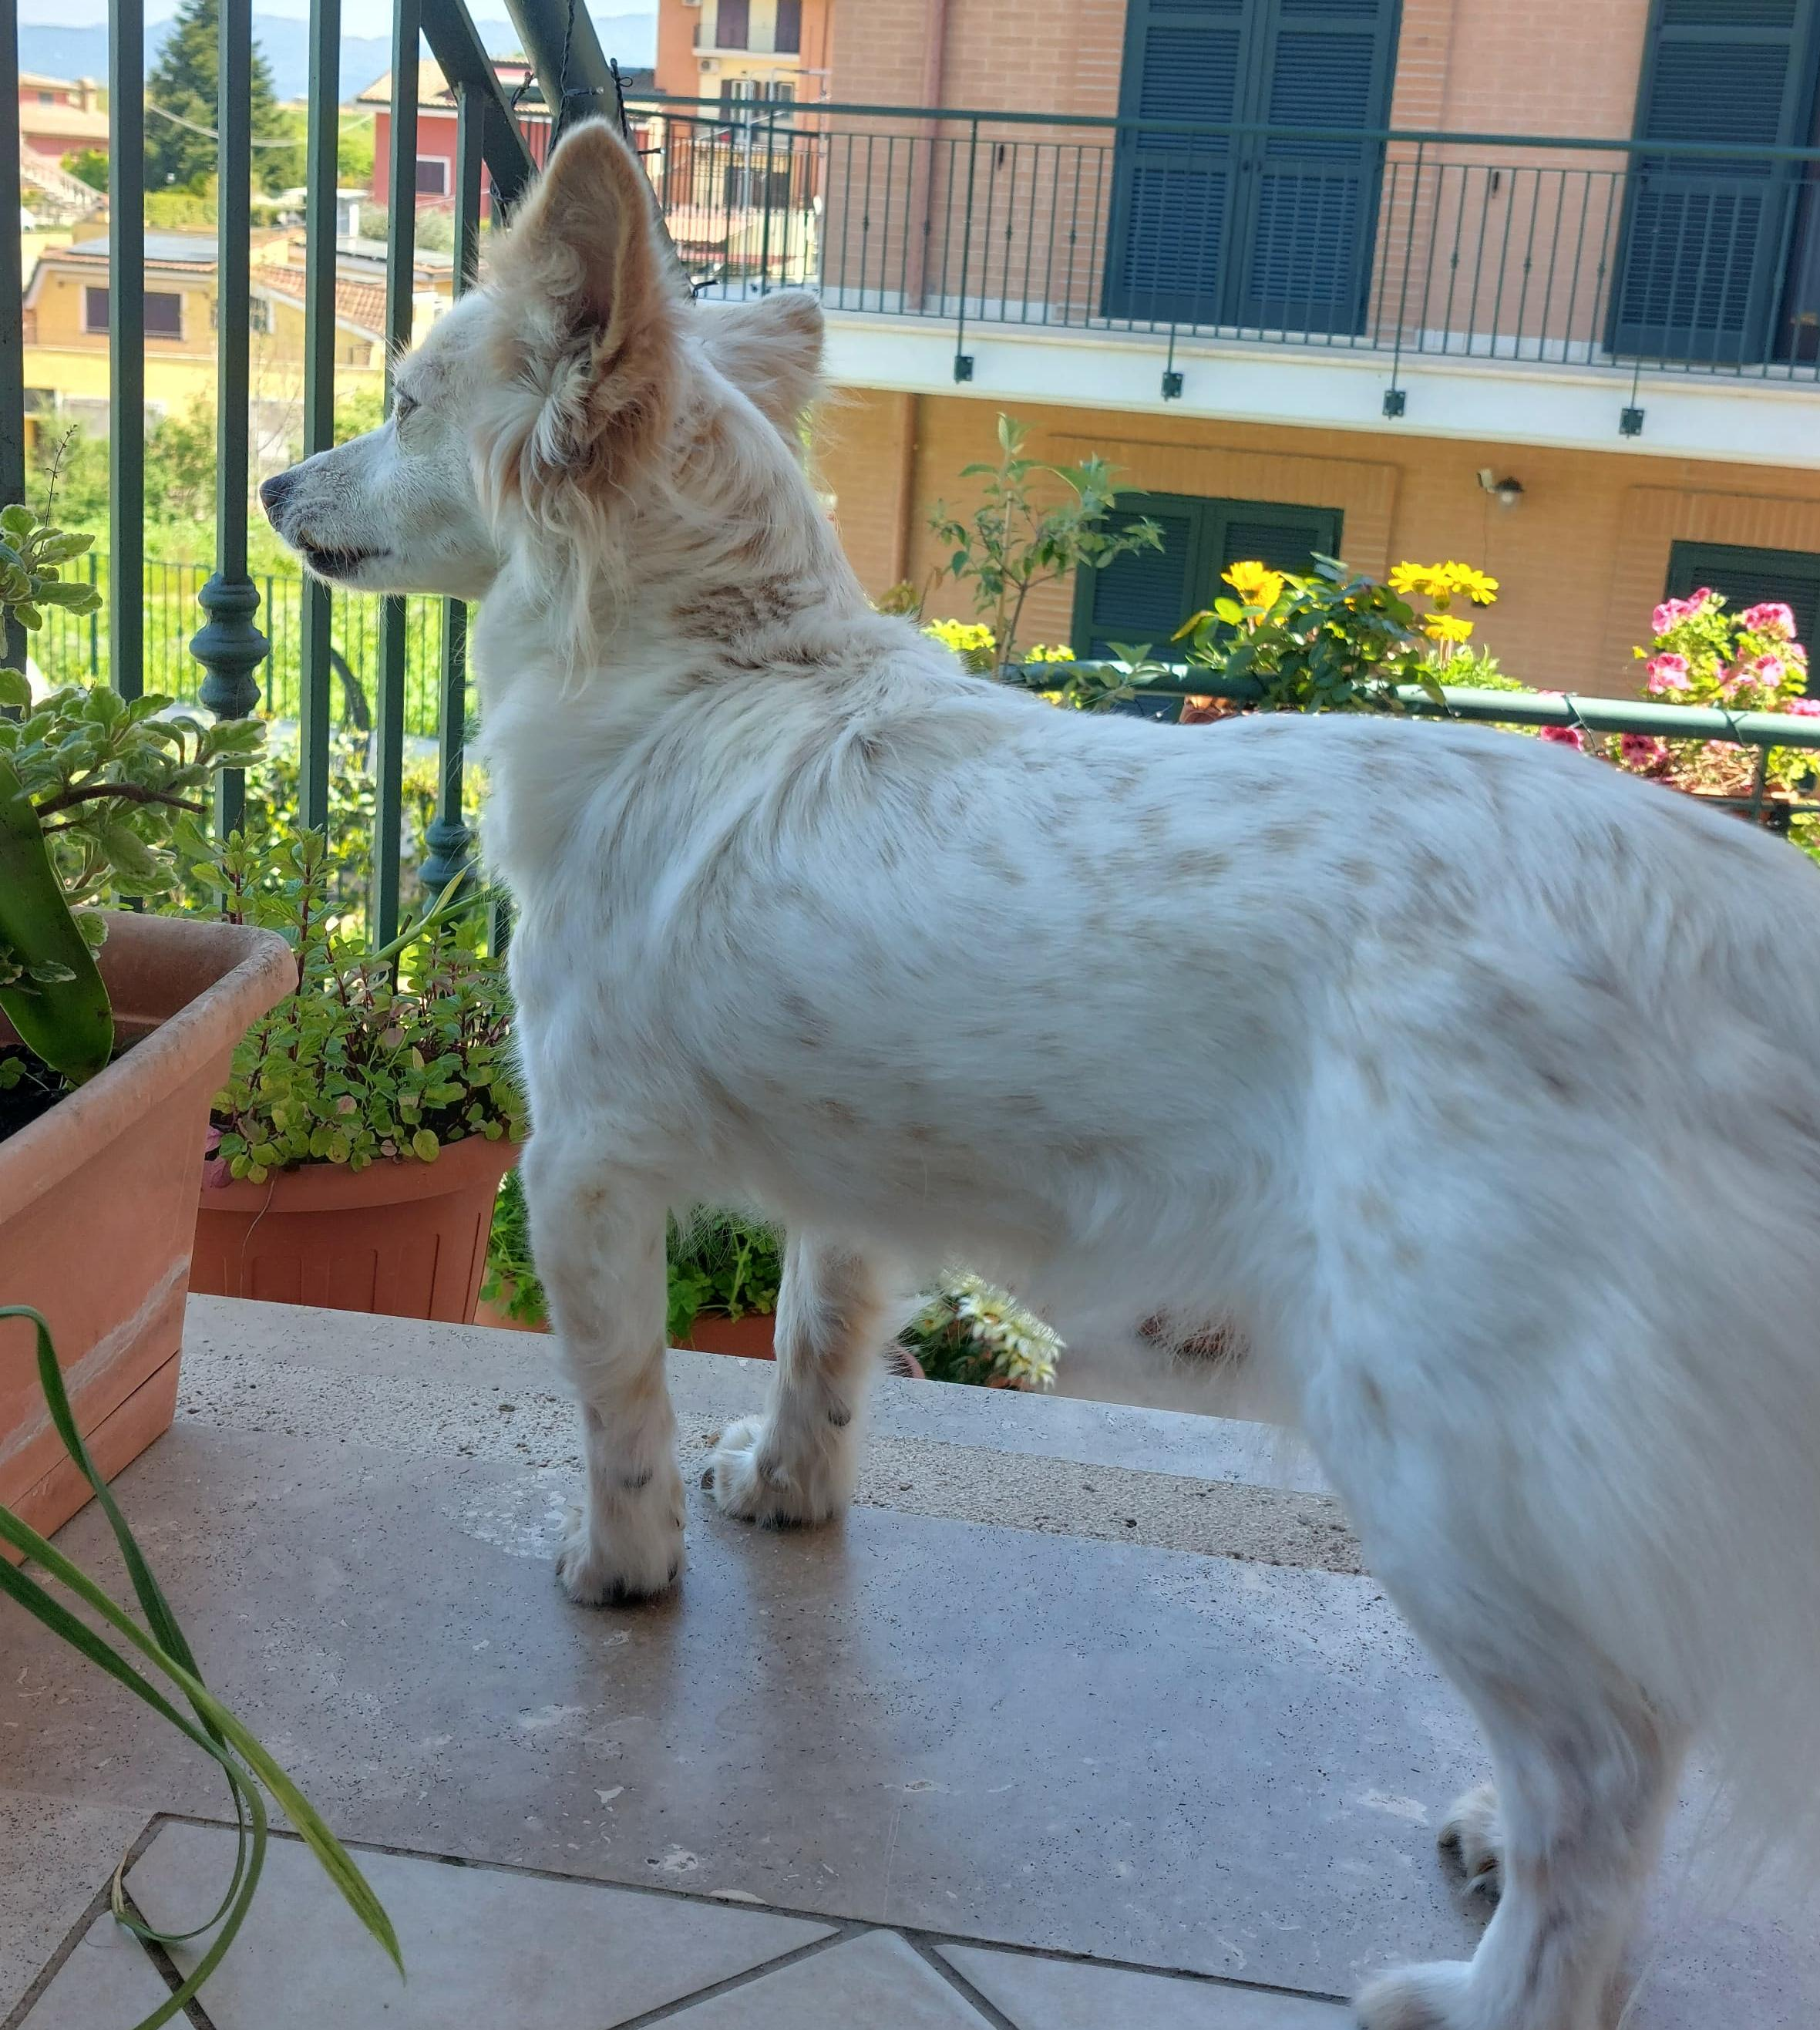
\includegraphics[width=\linewidth]{Figures/example.jpeg}
    \end{subfigure}
    \hspace{2cm}
    \begin{subfigure}[t]{0.4\linewidth}
        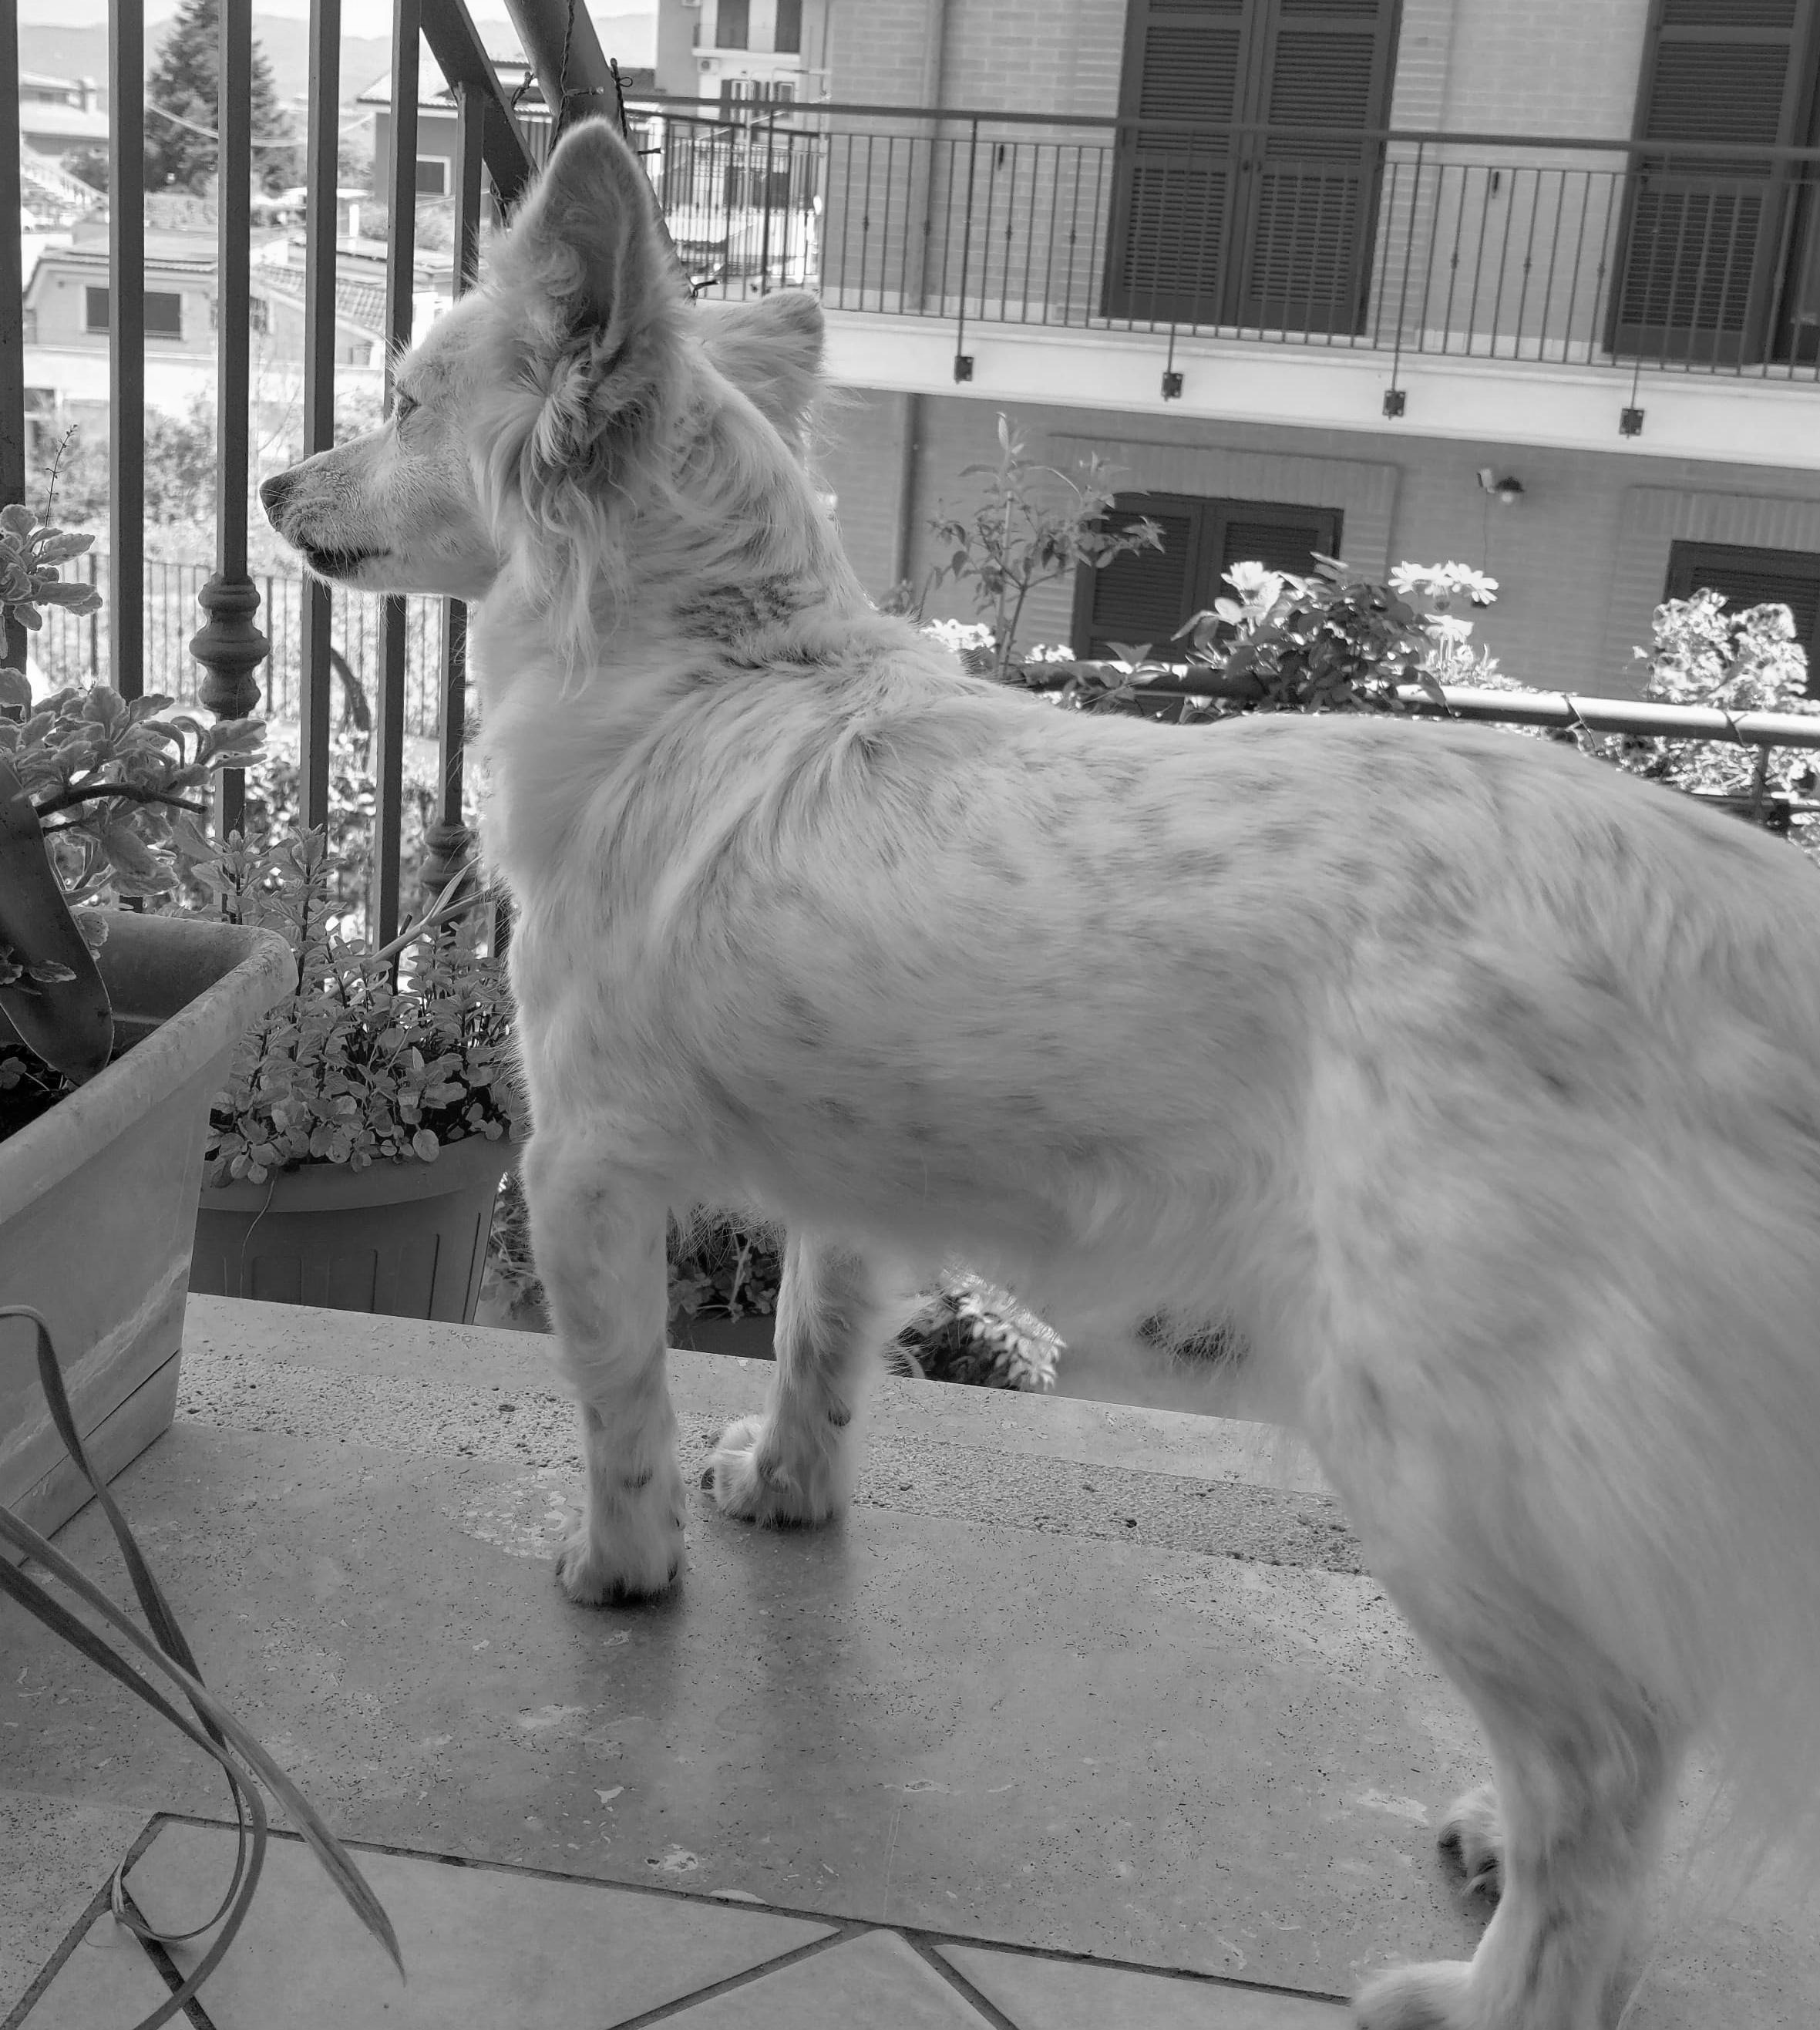
\includegraphics[width=\linewidth]{Figures/example_gray.jpeg}
    \end{subfigure}
\end{figure}
\subsection{Removing squares}
    One of the main challenges in processing and collecting the dataset concerns the cleanliness of the images, which can have significant impurities, such as the presence of squares on the sheets. It is essential to remove or mitigate these elements so that they blend in with the background and do not interfere with the analysis. Initially, the use of static techniques such as thresholding or the application of specific kernels to recognise the squares was considered. However, such techniques risked compromising the author's writing by erasing details. For this reason, it was decided to use compression techniques to detect patterns, since squares constitute a highly visible pattern that is more easily distinguishable by the machine than human handwriting.

    \paragraph{\gls{svd}}
    A first test involved examining the predominant patterns by means of a decomposition \gls{svd}. The image can be viewed as a matrix $H \times W$ of real values and can be decomposed into the product:
    \[
    	U\Sigma V^H = M
    \]
    where $M$ represents the image, $U$ and $V$ are unitary matrices ($UU^H = I$, same for $V$), $V^H$ is the Hermitian of $V$, and $\Sigma$ is a matrix $H \times W$ with only real values along the diagonal, called singular values.\
    It is possible to obtain a less detailed version of $M$ by cancelling some singular values of $\Sigma$, thus ignoring the contribution of certain patterns. It was observed that the predominant pattern (associated with the largest singular value) concerns squares, but its removal does not completely solve the problem, requiring the elimination of further patterns. The result obtained is encouraging, but entails a loss of information from human handwriting, as it too is present among the major patterns identified.

    \paragraph{\gls{fft}}
    An alternative idea is to perform a harmonic analysis of the images using \gls{fft}. The squares are repeated with a specific frequency along the two dimensions of the sheet and thus one can exploit their regular nature compared to human handwriting, which is less repetitive. Thus, one exploits both the difference between the regular patterns of the squares and the irregular strokes of the handwriting, as well as a greater capacity for compression than a simple pixel-by-pixel analysis.

    \noindent To verify this idea, we run a \gls{fft} on test images: a virtual sheet with only squares and the same sheet with drawings on it. In the case of the unmarked sheet, frequencies with larger amplitudes are mainly found aligned along the $x$ and $y$ axes (\cref{fig:synthetic_grid_fft}). By adding a pattern, the main frequencies remain almost the same (\cref{fig:synthetic_sign_fft}). To remove the squares, we remove these significant frequencies and reconstruct the image (\cref{fig:synthetic_clean_fft}).

    \begin{figure}
    	\centering
    	\begin{subfigure}[t]{\linewidth}
    		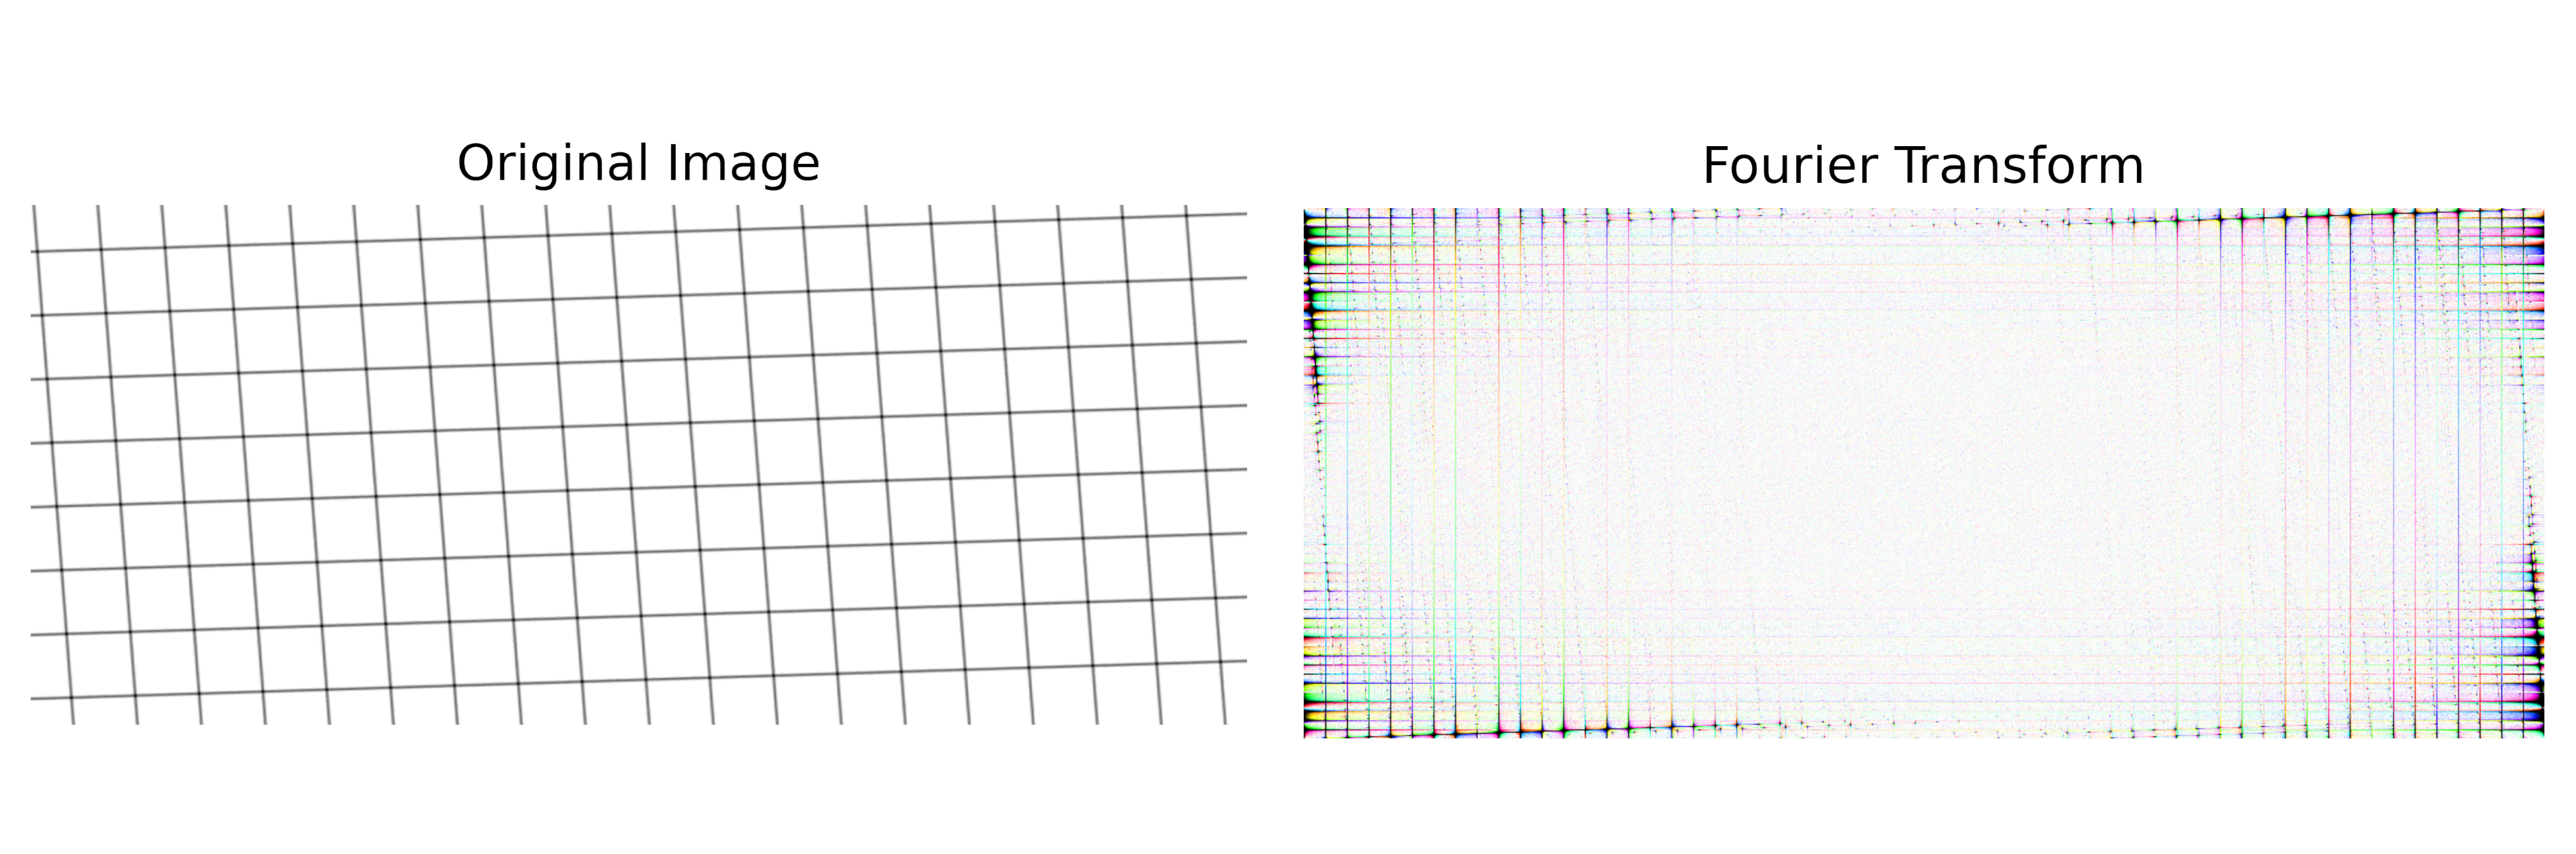
\includegraphics[width=\linewidth]{Figures/grid_fft.png} \caption{A slightly transformed grating, caused by an imperfect scan. The most significant frequencies are highlighted in black.} \label{fig:synthetic_grid_fft}
    	\end{subfigure}
    	\begin{subfigure}[t]{\linewidth}
    		\includegraphics[width=\linewidth]{Figures/test_fft.png} \caption{A deformed grating with a superimposed inscription. The frequencies of the lattice remain visible.} \label{fig:synthetic_sign_fft}
    	\end{subfigure} \begin{subfigure}[t]{\linewidth}
    		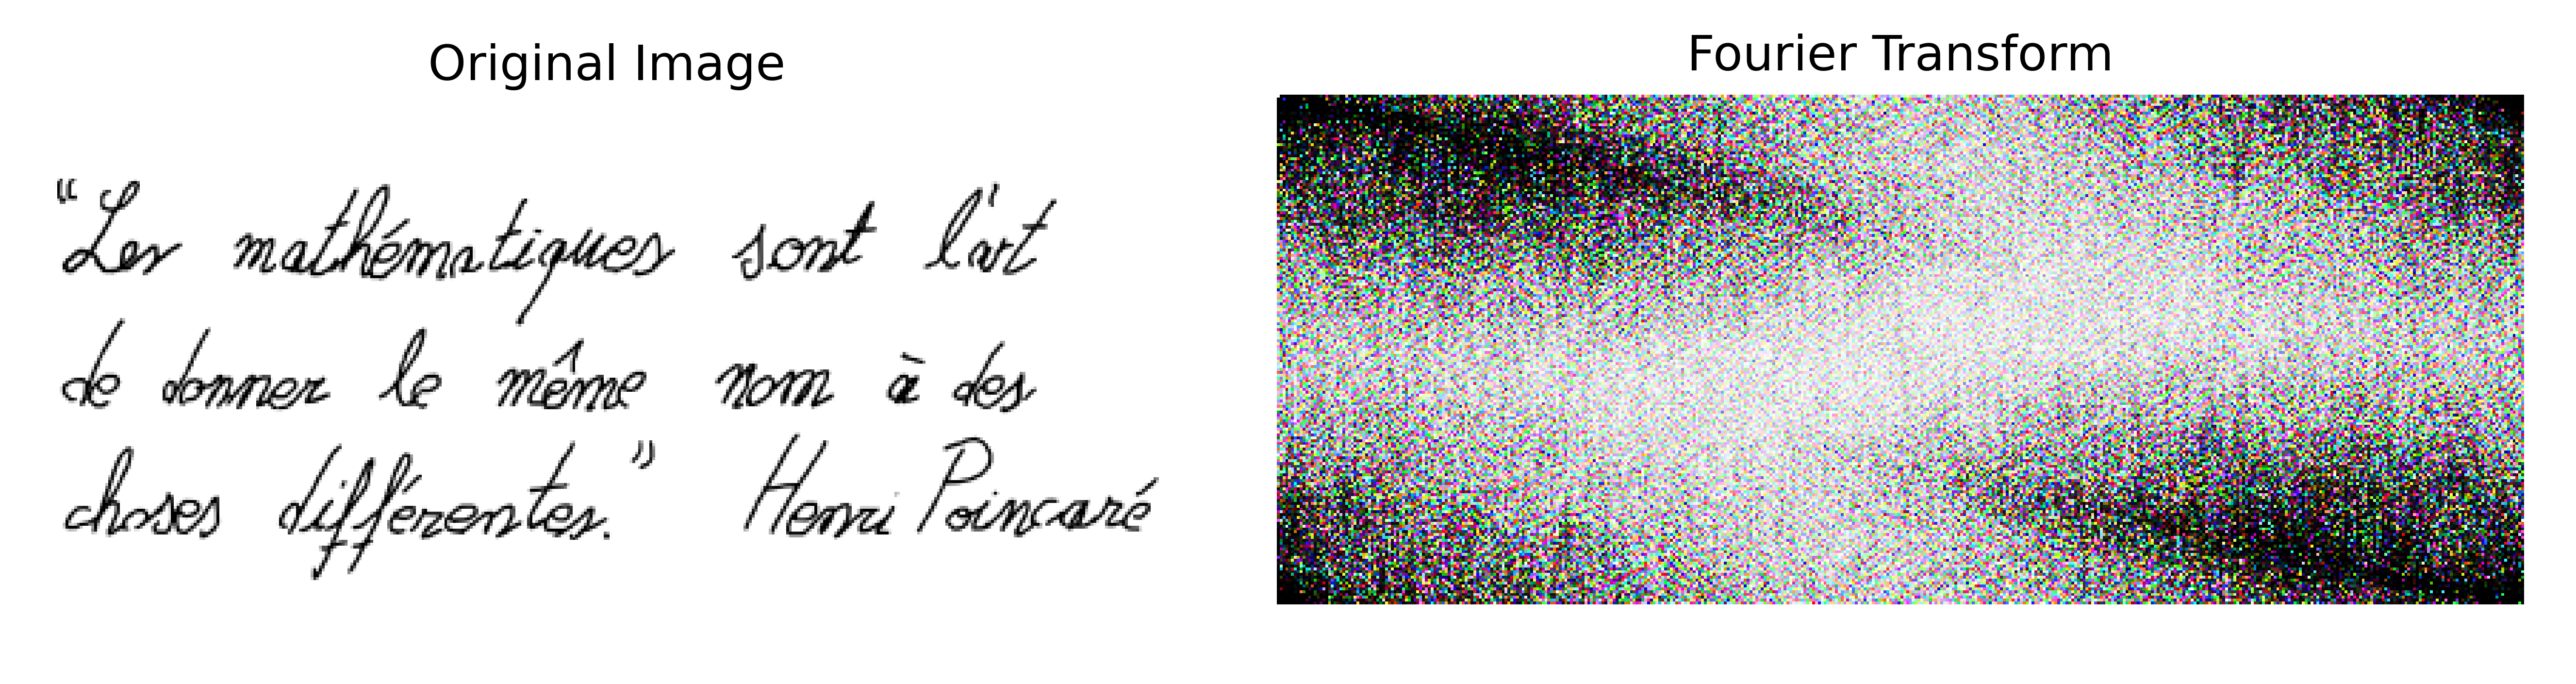
\includegraphics[width=\linewidth]{Figures/clean_fft.png} \caption{Lattice-less writing does not show significant Fourier coefficients, as recurring patterns are missing.} \label{fig:synthetic_clean_fft}
    	\end{subfigure}
    	\caption[Synthetic FFT test]{Fourier coefficient of the two-dimensional image. The squares show Fourier coefficients similar to those of the square waves: $\text{sqwave}(t) = \frac{4}{\pi}\sum_{k=1}^{\infty}\frac{\sin\left(2\pi(2k-1)t\right)}{2k-1}$. The most significant intensities are at regular intervals with decreasing intensities.}
    \end{figure}

    \noindent Empirically, by analysing $10$ randomly selected real images, it was observed that the squares were successfully removed without damaging the lettering, cancelling out the amplitudes corresponding to the first $5\%$ percentile of the most significant frequencies.

    \noindent However, this process introduces an issue of colour distortion. In the original image, the grey levels were distributed intuitively: most of the pixels were white, with only a small portion in darker shades of grey, representing the writing. After reconstructing the image using the FFT, a significant number of pixels took on intermediate shades of grey that weren't present before. This affects the clarity of the image, especially by blending the background and the lettering, making it harder to distinguish between the important features from the unwanted noise.

	\noindent To reduce the effects of this distortion, we adopted a colour normalisation approach to keep the grey values as close as possible to the original image. The main idea was to identify extremely light and extremely dark grey values in the original image and to expand the range of grey values in the reconstructed image to match them.

    \noindent It was observed that, in the original image, pixels with a grey level below $0.2$ certainly belong to the lettering, while those with a grey level above $0.8$ correspond to the white background of the page. Consequently, the pixels of the lettering and white background in the original image are counted. In the cleaned image, the darkest pixels (with a grey value below $0.2$ in the original image) are assigned to black, while the lightest pixels (with a grey value above $0.8$ in the original image) are assigned to white.

    \noindent To correct the distortion, we expanded the grey values of the reconstructed image so that pixels that should be black became darker and those that should be white became lighter. We then clamped these values within natural limits (0 to 1) to avoid out-of-scale colours. This process was called ‘clamp normalisation’. A result of this procedure is shown in \cref{fig:first_reconstruct}.

    \begin{note} Presente nel capitolo Results \end{note}

    \begin{algorithm}[h]
    	\caption[Cleaning procedure using FFT]{Cleaning procedure using FFT.\\
    		\begin{minipage}[t]{\linewidth}
    			\textsc{INPUT}
    			\begin{itemize}[noitemsep, topsep=0pt]
    				\item[$\mathcal{I}$:] Image as matrix $W\times H$ in gray scale
    				\item[$p$:] percentile of significant magnitudes
    				\item[$a$:] thresholds $(\min, \max)$
    			\end{itemize}
    			\textsc{OUTPUT} $\mathcal{I}_{\text{new}}$: Image as matrix $W\times H$ in gray scale
    		\end{minipage}
    	}
    	\begin{algorithmic}[1]
    		\Procedure{CleanFFT}{$\mathcal{I}, p, a$}
    		\State $\hat{\mathcal{I}} \gets \text{normalize}\left(\mathcal{I}\right)$
    		\State $F_{\hat{\mathcal{I}}} \gets \text{fft2d}\left(\hat{\mathcal{I}}\right)$
    		\State $f = (f_1, \dots, f_{W\times H}) \gets \text{argsort}\left(\text{flatten}\left(F_{\hat{\mathcal{I}}}\right), \text{rule=abs}\right)$
    		\State $f_{\text{best}} \gets f\left[\text{last}\; \lfloor{p\cdot\text{length}\rfloor}\;\text{values}\right]$ \Comment{components with high magnitude}
    		\For{$k \in f_{\text{best}}$}
    			\State $F_{\hat{\mathcal{I}}}[k] = 0.0$
    		\EndFor
    		\State $\hat{\mathcal{I}} \gets \text{ifft2d}\left(F_{\hat{\mathcal{I}}}\right)$ \Comment{rebuild normalized image}
    		\State $w_{\text{cnt}} \gets \textbf{count}\;\mathcal{I} \geq a(\max)$ \Comment{normalization using dilation and clamp}
    		\State $b_{\text{cnt}} \gets \textbf{count}\;\mathcal{I} \leq a(\max)$
    		\State $h_{w} \gets \max_{w_{\text{cnt}}^{\mathrm{-th}}}\mathcal{\hat{I}}$
    		\State $h_{w} \gets \min_{b_{\text{cnt}}^{\mathrm{-th}}}\mathcal{\hat{I}}$
    		\State $\mathcal{I}_{\text{new}} \gets \frac{\mathcal{\hat{I}} - h_{b}}{h_{w}-h_{b}}$
    		\Where{$\mathcal{I}_{\text{new}} > 1$, $\mathcal{I}_{\text{new}} = 1$}
    		\Where{$\mathcal{I}_{\text{new}} < 0$, $\mathcal{I}_{\text{new}} = 0$}
    		\State \Return $\mathcal{I}_{\text{new}}$
    		\EndProcedure
    	\end{algorithmic}
    	\label{alg:CleaningFFT}
    \end{algorithm}


% synthesis algorithm
\section{Synthesis}
The tessellation phase extracts tiles $N\times N$ from each image. Starting from a matrix of grey pixels, represented as a matrix in $\left[0,1\right]^{h \times w}$, where $h$ is the height and $w$ the width of the image.

\noindent Al termine di questa procedura, ogni immagine viene rappresentata come un elenco di tessere, motivo per cui questa fase è chiamata "sintesi": infatti, risulta difficile ricostruire l'immagine originale a partire dalle tessere. Questo processo complica notevolmente qualsiasi tentativo di falsificazione dell'opera, poiché ricostruire manualmente un'immagine con una distribuzione di tessere simile a quella originale è estremamente complicato. Inoltre, la dimensione delle tessere nella rappresentazione è ridotta, ma sufficientemente grande da catturare piccoli automatismi della mano dell'autore, dettagli che sono difficilmente riproducibili in modo volontario.

\begin{algorithm}[ht]
\caption{Algorithm for tile extraction}
\begin{algorithmic}[1]
\Function{TilesExtraction}{$\textnormal{M}, \textnormal{h}, \textnormal{w}$}
    \State declare $v$ as matrix $N \times N$ \Comment{$N$ is size of tiles}
    \State $L \gets \texttt{empty list}$ \Comment{will have $(\textnormal{h} - N + 1)\times(\textnormal{w} - N+1)$ elements}
    \For{$row \gets 0$ to $\textnormal{h} - N$, $col \gets 0$ to $\textnormal{w} - N$}
        \For{$i \gets 1$ to $N$, $j \gets 1$ to $N$}
            \State $v[i][j] \gets \textnormal{M}[row + i][col + j]$
        \EndFor
        \State call \texttt{Append}($L$, $v$)
    \EndFor
\EndFunction
\label{alg:SequentialTilesExtraction}
\end{algorithmic}
\end{algorithm}

\begin{figure}[ht]
    \centering
    \begin{subfigure}{0.4\linewidth}
        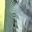
\includegraphics[width=\linewidth]{Figures/example_detail.png}
        \caption{Image detail $32 \times 32$.}
    \end{subfigure}
    \hspace{2cm}
    \begin{subfigure}{0.4\linewidth}
        
\includegraphics[width=\linewidth]{Figures/example_tiles.png}
        \caption{List of tiles $8 \times 8$.}
    \end{subfigure}
    \caption[Illustration of synthesis process]{The synthesis process convert an image in a list of its tiles.}
    \label{fig:puffer_tiles}
\end{figure}


% comparison and theory
\section{Comparison}
\begin{modified}
In order to compare two works, we decided to use the clustering \gls{fcm}, which is less sensitive to potential noise. This is particularly important in our case, as the comparison between two works leverages areas with lower densities, where noise could significantly affect the results.

\noindent In the previous study (\cite{thesis}), it was observed that the formula for comparing works was highly influenced by tiles with fewer occurrences. In our current context, which operates in a continuous space, these tiles correspond to regions with lower densities.

\noindent In this thesis, I developed an algorithm for comparing works and demonstrated its application through an example to better investigate its characteristics.
\end{modified}

\paragraph{Comparison value using \gls{kmeans}}
\begin{modified} As already mentioned in \cref{chap:LiteratureReview}, we compared two works using their synthesized tiles. Specifically, we extracted two sets of tiles, $\mathcal{A},\mathcal{B}$, from the two works, where each tile is represented as a vector in $\mathbb{R}^K$. In \cite{thesis}, we employed predefined boxes to cluster the tiles. Each box had the same measure but contained a different number of data points (i.e., tiles). To analyze these clusters, we used a clustering algorithm, \gls{kmeans}, as described in \cref{chap:LiteratureReview}. Each cluster represents a region in the space $\mathbb{R}^K$ with its own measure and weights respect $\mathcal{A}, \mathcal{B}$.

\noindent The clustering procedure using \gls{kmeans} can be summarized as follows:
\begin{enumerate}
	\item Compute the \gls{kmeans} clustering of $\mathcal{L}:=\mathcal{A}\cup\mathcal{B}$. This gives the predictor $\mathcal{P}$, where $\mathcal{P}(x)$ is the centroid of the data point $x$.
	\item Compute the measure of each cluster: $\mu(c)=\sqrt{\mathbb{E}_{x\sim\mathcal{L}}\left[\left|x-c\right\|^2\middle| \mathcal{P}(x)=c\right]}^K$ where $c$ is the centroid of the cluster.
	\item Compute the weight of each cluster with respect to $\mathcal{A}$: $p_\mathcal{A}(c)=\mathbb{P}_{x\sim\mathcal{A}}\left[\mathcal{P}(x)=c\right]$
	\item Compute the weight of each cluster with respect to $\mathcal{B}$: $p_\mathcal{B}(c)=\mathbb{P}_{x\sim\mathcal{B}}\left[\mathcal{P}(x)=c\right]$
	\item Compute the Jaccard Index:
	\begin{align*}
		D_\mathcal{A} &:= \texttt{clusters containing tiles from $\mathcal{A}$}\\
		D_\mathcal{B} &:= \texttt{clusters containing tiles from $\mathcal{B}$}\\
		\left|D_\mathcal{A}\cup D_\mathcal{B}\right| &= M \quad \texttt{(total number of clusters)} \\
		\left|D_\mathcal{A}\cap D_\mathcal{B}\right| &= \texttt{clusters containing tiles from both $\mathcal{A}$ and $\mathcal{B}$} \\
		J_{\mathcal{A},\mathcal{B}} &:= \frac{\left|D_\mathcal{A}\cap D_\mathcal{B}\right|}{\left|D_\mathcal{A}\cup D_\mathcal{B}\right|}
	\end{align*}
	\item Compute the measure of all clusters: $\mu(D_\mathcal{A}\cup D_\mathcal{B}) = \sum_{c\in D_\mathcal{A}\cup D_\mathcal{B}} \mu(c)$
	\item Compute the comparison value between the two works:
	\[
		d_{\gls{kmeans}}(\mathcal{A},\mathcal{B}) = \left(1+J_{\mathcal{A},\mathcal{B}}\right)^{-1}\frac{1}{\mu(D_\mathcal{A}\cup D_\mathcal{B})}\sum_c \mu(c)\left(\frac{p_\mathcal{A}(c)-p_\mathcal{B}(c)}{p_\mathcal{A}(c)+p_\mathcal{B}(c)}\right)^2
	\]
\end{enumerate}
\end{modified}

\subsection{Comparison value using \gls{fcm}}
\begin{modified}
\noindent Next, we will apply \gls{fcm} to the fused distribution $\mathcal{L}$. Using fuzzy clustering, each data point will be assigned a degree of membership to multiple clusters, allowing for a more flexible representation of the data. For each cluster with centroid $c$, we will compute its size $\mu(c)$ and the weights of the set of samples, $p_\mathcal{A}(c)$ and $p_\mathcal{B}(c)$. Finally, we will redefine the Jaccard index between $D_\mathcal{A}$ and $D_\mathcal{B}$ within a fuzzy logic framework to better capture the similarities between the two sets.

\noindent The fuzzy nature of \gls{fcm} requires a redefinition of the cluster measure. Unlike \gls{kmeans}, where each data point is assigned to a single cluster by the predictor $\mathcal{P}$, in \gls{fcm} each data point has a degree of membership in multiple clusters. To extend the concept of cluster size, we define the measure of a cluster as a quantity proportional to the $K$ dimensional hypervolume of a hypersphere with radius equal to the mean square distance of the data from its centroid. For \gls{kmeans} this is expressed as:
\begin{equation*}
	\mu(c) = {\sqrt{\mathbb{E}_{x\sim\mathcal{L}}\left[\left\|x-c\right\|^2\middle|\mathcal{P}(x)=c\right]}\,}^{K} = {\sqrt{\frac{1}{\left|\{x\middle|\mathcal{P}(x)=c\}\right|}\sum_{x:\mathcal{P}(x)=c}\left\|x-c\right\|^2}\,}^{K}
\end{equation*}

\noindent In \gls{kmeans}, the algorithm aims to minimise the loss function:
\[
	\sum_c\sum_{x:\mathcal{P}(x)=c}\left\|x-c\right\|^2
\]
We get a different perspective of this loss function:
\begin{align*}
	\sum_c\sum_{x:\mathcal{P}(x)=c}\left\|x-c\right\|^2 &= \sum_c\left|\{x:\mathcal{P}(x)=c\}\right|\frac{1}{\left|\{x:\mathcal{P}(x)=c\}\right|}\sum_{x:\mathcal{P}(x)=c}\left\|x-c\right\|^2 \\
	&= N\sum_c\frac{\left|\{x:\mathcal{P}(x)=c\}\right|}{N}\mathbb{E}_{x\sim\mathcal{L}}\left[\left\|x-c\right\|^2\middle|\mathcal{P}(x)=c\right] \\
	&= N\sum_c\mathbb{P}_{x\sim\mathcal{L}}\left[\mathcal{P}(x)=c\right]\mathbb{E}_{x\sim\mathcal{L}}\left[\left\|x-c\right\|^2\middle|\mathcal{P}(x)=c\right] \\
	&= N\sum_c p(c)E(c)
\end{align*}
where $p(c):= \mathbb{P}_{x\sim\mathcal{L}}\left[\mathcal{P}(x)=c\right]$ and $E(c):= \mathbb{E}_{x\sim\mathcal{L}}\left[\left\|x-c\right\|^2\middle|\mathcal{P}(x)=c\right]$

\bigskip\noindent Extending this idea, we generalize the concept using the objective function of \gls{fcm}, as defined in \cref{def:fuzzyloss}. This allows the introduction of fuzzy membership.
\begin{definition}[cluster's values]
\label{def:cluster_values}
	Applying \gls{fcm} to the data set $\mathcal{S}$ with weights $w$ and tiles in $\mathbb{R}^K$, we obtain the centroids $\mathcal{C}$ and the memberships $\mu_c(x)$.

	\noindent We call the representability of cluster with centroid $c$ respect all other clusters the value: $p(c) = \frac{\sum_x w_x\mu_x(c)}{\sum_x w_x}$

	\noindent We call the concentration of cluster with centroid $c$ respect the membership measure the value: $\sigma(c) = \frac{\sum_x w_x\mu_x(c)^2}{\sum_x w_x\mu_x(c)}$
	\begin{remark}
		$\sigma(c)\in\left(0,1\right]$ because $\mu_x(c)\leq1$ and so: $\sum_x w_x\mu_x(c)^2 \leq \sum_x w_x\mu_x(c)$
	\end{remark}

	\noindent We call the mean square radius of the cluster with centroid $c$ the value: \\$E(x) = \frac{\sum_x w_x\mu_x(c)^2\left\|x-c\right\|^2}{\sum_x w_x\mu_x(c)^2}$

	\noindent The loss function of algorithm \gls{fcm} is can rewritted as:
	\[
		\mathcal{L}_\mathcal{S}(\mathcal{C}) = \sum_x w_x\sum_c p(c)\sigma(c)E(c)
	\]

	\noindent We denote by $\mu(c)$ the measure of the cluster $c$ as:
	\begin{equation}
		\label{def:cluster_measure}
		\mu(c) = \sigma(c)E(c)^{K/2} = \frac{\sum_x w_x\mu_x(c)^2}{\sum_x w_x\mu_x(c)}{\sqrt{\frac{\sum_{x\in\mathcal{S}} w_x\mu_x(c)^2 \left\|x-c\right\|^2}{\sum_{x\in\mathcal{S}}w_x\mu_x(c)^2}}\,}^K
	\end{equation}
\end{definition}
\end{modified}

\bigskip \noindent Similarly, we can define the values of the sets of tiles on the centroids:
\begin{toReview}
\begin{definition}
	\label{def:weightovercluster}
	Given a merged data set $\mathcal{S}=\mathcal{A}+\mathcal{B}$, where tiles belong in $\mathbb{R}^K$, and weights $w_\mathcal{A}$ and $w_\mathcal{B}$, the application of \gls{fcm} yields the set of centroids $\mathcal{C}$ and the membership degrees $\mu_c(x)$ for each data point $x\in\mathcal{S}$.

	\noindent The representability of the set $\mathcal{A}$ with respect to a centroid $c$ is defined as
	$$ p_\mathcal{A}(c) = \frac{\sum_{x\in\mathcal{A}} w_x\mu_x(c)}{\sum_{x\in\mathcal{A}} w_x} $$

	\noindent Similarly, the representability of the set $\mathcal{B}$ with respect to a centroid $c$ is defined as
	$$ p_\mathcal{B}(c) = \frac{\sum_{x\in\mathcal{B}} w_x\mu_x(c)}{\sum_{x\in\mathcal{B}} w_x} $$
\end{definition}

\noindent In this way, we have defined both the cluster measures and the weights of each cluster for the sets of tiles $\mathcal{A}$ and $\mathcal{B}$. This completes part of the comparison formula, leaving the inclusion of the Jaccard index $J_{\mathcal{A},\mathcal{B}}$ as the next step:
\[
	\frac{1}{\mu(D_\mathcal{A} \cup D_\mathcal{B})} \sum_c \mu(c) \left(\frac{p_\mathcal{A}(c) - p_\mathcal{B}(c)}{p_\mathcal{A}(c) + p_\mathcal{B}(c)}\right)^2
\]
\end{toReview}

\paragraph{fuzzy logic and the Jaccard Index}
\begin{toReview}
\noindent Defining the Jaccard index in fuzzy logic is a non-trivial task because the cardinality of a set is not defined in the same way as in Boolean logic. Unlike Boolean logic, where membership has a binary truth value (true or false), in fuzzy logic, membership degrees are continuous.

\noindent Even if \gls{fcm} is requested to produce $M$ centroids, not all clusters necessarily "exist". In Boolean logic, a cluster exists if at least one data point belongs to it. In fuzzy logic, however, no data point fully belongs to a specific cluster, and a data point can belong to multiple clusters simultaneously to varying degrees. Thus, the truth value of the statement "\texttt{$x$ belongs to the cluster with centroid $c$}" is $\mu_x(c)$. Extending this concept, the truth value of the existence of a cluster with centroid $c$ must also be defined. While there is no unique answer, we seek an acceptable and consistent definition for this operation.

\noindent Let $D_\mathcal{A}$ denote the set of clusters containing at least one data point from $\mathcal{A}$, and $\mu_c(D_\mathcal{A})$ represent the degree to which the cluster with centroid $c$ exists within $\mathcal{A}$. Similarly, $\left|D_\mathcal{A}\right|$ represents the cardinality of the set of clusters, but in fuzzy logic, this cardinality is not an integer and can take continuous values. Below, we provide formal definitions for these concepts.

\begin{definition}(Jaccard index)
	\label{def:Jaccard_fcm}
	In fuzzy logic, the truth value of a logical disjunction is defined as the maximum of the truth values of its individual propositions. Based on this, the degree to which the cluster with centroid $c$ exists in $A$ is given by:
	$$\mu_c(D_\mathcal{A}) = \max_{x\in\mathcal{A}}\mu_x(c)$$

	\noindent The cardinality of a set is defined as the sum of the membership degrees of all data points to the set. Thus, the cardinality of $D_\mathcal{A}$ is:
	$$|D_\mathcal{A}| = \sum_c \mu_c(D_\mathcal{A})$$

	\noindent Consequently, the cardinality of the union of $D_\mathcal{A}$ and $\mathcal{B}$ is:
	$$|D_\mathcal{A} \cup D_\mathcal{B}| = \sum_c \mu_c(D_\mathcal{A} \cup D_\mathcal{B}) = \sum_c \max\{\mu_c(D_\mathcal{A}), \mu_c(D_\mathcal{B})\} $$

	\noindent Similarly, the cardinality of the intersection of $D_\mathcal{A}$ and $D_\mathcal{B}$ is derived from the logical conjunction, which uses the minimum:
	$$|D_\mathcal{A} \cap D_\mathcal{B}| = \sum_c \mu_c(D_\mathcal{A} \cap D_\mathcal{B}) = \sum_c \min\{\mu_c(D_\mathcal{A}), \mu_c(D_\mathcal{B})\} $$

	\noindent Based on these definitions, the Jaccard index for fuzzy logic is given by:
	\begin{equation*}
		J_{D_\mathcal{A},D_\mathcal{B}} :=
		\frac{
			\left|D_\mathcal{A} \cap D_\mathcal{B}\right|
		}{
			\left|D_\mathcal{A} \cup D_\mathcal{B}\right|
		}
		= \frac{
			\sum_c \min \left\{
				\max_{x\in \mathcal{A}}\left(
					\mu_x\left(c\right)
				\right), \max_{x\in \mathcal{B}}\left(
					\mu_x\left(c\right)
				\right)
			\right\}
		}{
			\sum_c \max\left\{
				\max_{x\in \mathcal{A}}\left(
					\mu_x\left(c\right)
				\right),\max_{x\in \mathcal{B}}\left(
					\mu_x\left(c\right)
				\right)
			\right\}
		}
	\end{equation*}
\end{definition}
\end{toReview}

\noindent The definitions provided in \cref{def:weightovercluster,def:cluster_measure,def:Jaccard_fcm} are sufficient to formulate the distance between two proposed samplings based on \gls{fcm}:
\[
d_{\text{\gls{fcm}}}\left(\mathcal{A},\mathcal{B}\right) = \left(1+J_{\mathcal{A},\mathcal{B}}\right)^{-1}\frac{1}{\mu(D_\mathcal{A} \cup D_\mathcal{B})} \sum_c \mu(c) \left(\frac{p_\mathcal{A}(c) - p_\mathcal{B}(c)}{p_\mathcal{A}(c) + p_\mathcal{B}(c)}\right)^2
\]


\subsection{Algorithm}
The algorithm initially involves applying \gls{fcm} to the fused dataset of the two works, in order to define the size and discretisation of the space of the tiles.
\begin{itemize}
	\item $ \mu(c) = \frac{\sum_x w_x\mu_x(c)^2}{\sum_x w_x\mu_x(c)}\sqrt{\frac{\sum_{x\in\mathcal{S}} w_x\mu_x(c)^2 \|x-c\|^2}{\sum_{x\in\mathcal{S}}w_x \mu_x(c)^2}\,}^K $
	\item $ p_\mathcal{A}(c) = \frac{\sum_{x\in \mathcal{A}} w_x\mu_x(c)}{\sum_{x\in \mathcal{A}}w_x} $ and similarly $ p_B(c) = \frac{\sum_{x\in \mathcal{B}} w_x\mu_x(c)}{\sum_{x\in \mathcal{B}}w_x} $
	\item $ J_{D_\mathcal{A}, D_\mathcal{B}} $ as in \cref{def:Jaccard_fcm}
\end{itemize}
The distance between works will be defined as:
\begin{equation}
\label{eq:fuzzy_distance}
	d_{\gls{fcm}}(A, B) = (1 + J_{D_A, D_B})^{-1}\frac{\sum_c  \mu(c)\left(\frac{p_\mathcal{A}(c)-p_\mathcal{B}(c)}{p_\mathcal{A}(c)+p_\mathcal{B}(c)}\right)^2}{\sum_c \mu(c)}
\end{equation}

\begin{modified}
\noindent A simple application for a synthetic dataset is shown below, where we compare three methods for clustering and comparing two distributions $\mathcal{A}$ and $\mathcal{B}$. The three methods are:
\begin{itemize}
	\item \textbf{Box-clustering}: the space is partitioned into fixed, predefined boxes.
	\item \textbf{\gls{kmeans}}: the space is divided into circular clusters, where each cluster is defined by its centroid and radius.
	\item \textbf{\gls{fcm}}: the space is divided into fuzzy circular clusters, where each data point has a degree of membership to multiple clusters.
\end{itemize}

\noindent To illustrate these approaches, we generate two synthetic datasets $\mathcal{A}$ and $\mathcal{B}$ in a two-dimensional space. Each dataset consists of $150$ data points randomly sampled from six Gaussian distributions, with the addition of uniform noise. We cluster the merged dataset into $4$ clusters using each of the three methods.

\noindent In \cref{fig:box_clustering}, we show the box-clustering method, where the space is divided into a grid of fixed-size boxes, and each box contains a certain number of points from $\mathcal{A}$ and $\mathcal{B}$. In \cref{fig:kmeans_clustering}, we apply \gls{kmeans}, where the clusters are represented as circular regions centered at their respective centroids. Finally, in \cref{fig:fcm_clustering}, we use \gls{fcm} to produce fuzzy clusters, where the degree of membership of each data point is visualized using a color map.

\begin{figure}[p]
	\centering
	\begin{subfigure}{0.48\linewidth}
		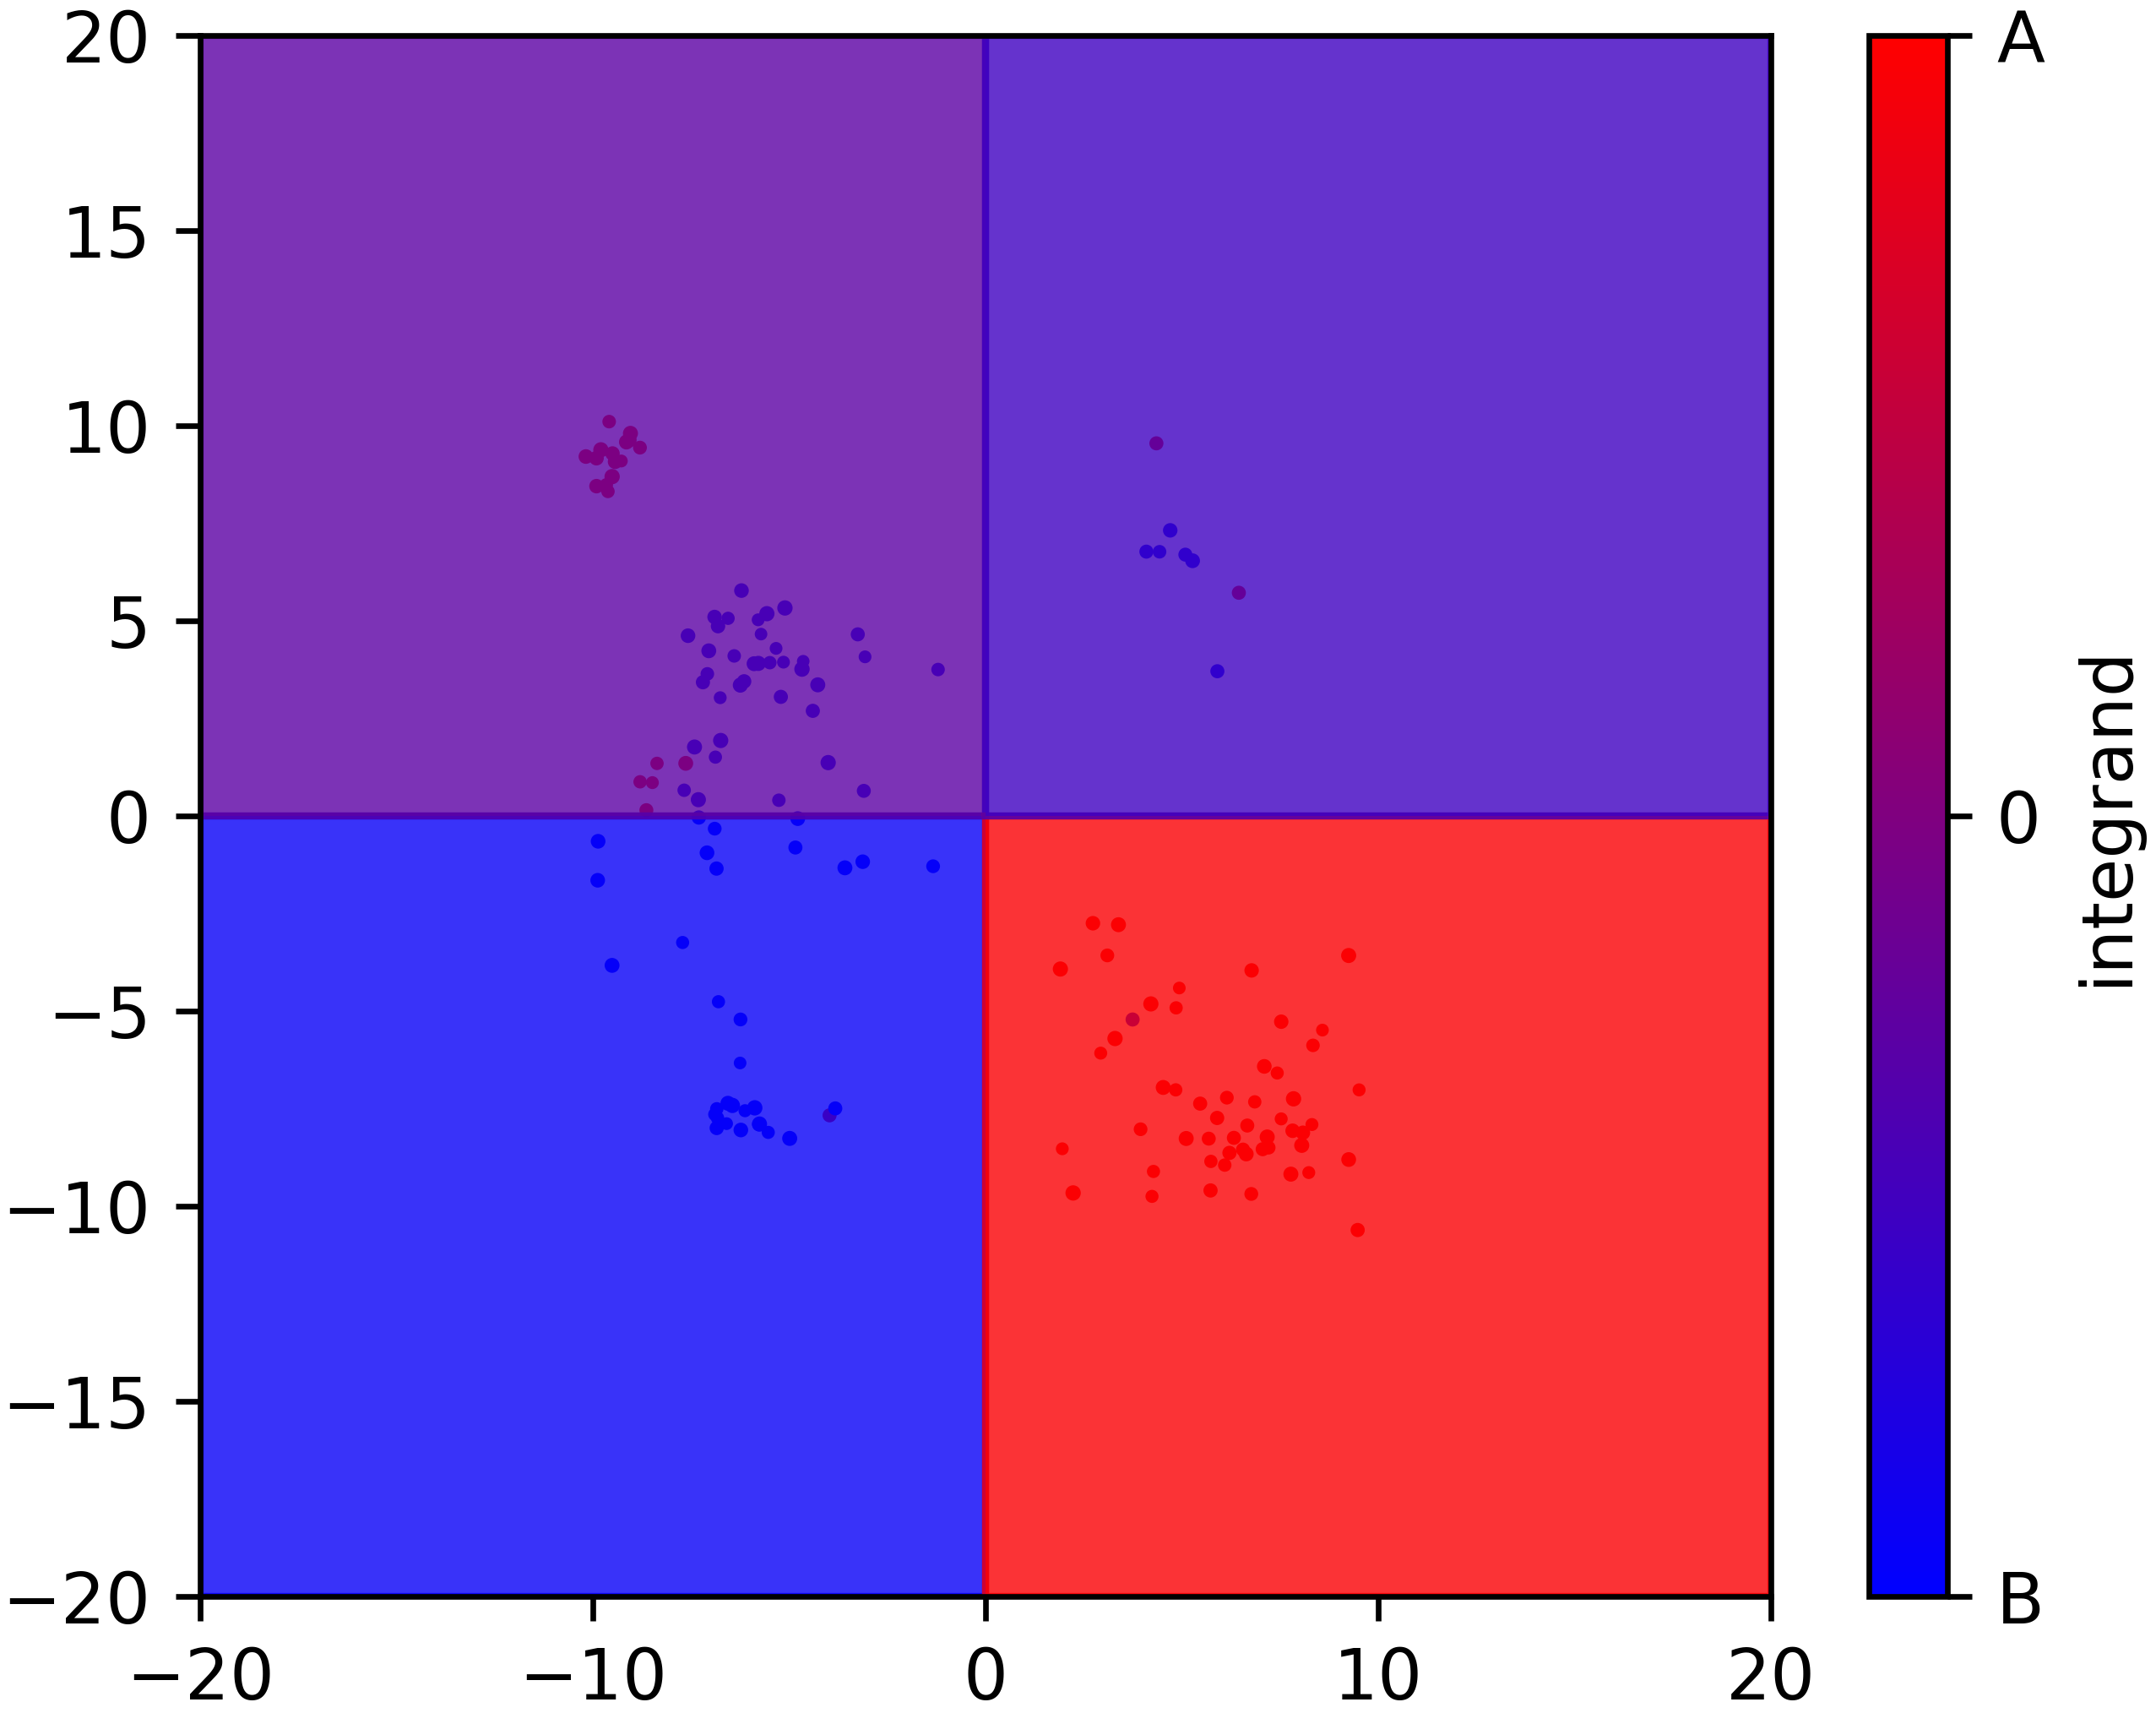
\includegraphics[width=\linewidth]{Figures/box_comparison.png}
		\caption[Box clustering, example of comparison]{Box clustering using $4$ boxes.\\ Computed distance: $0.268$.}
		\label{fig:box_clustering}
	\end{subfigure}
	\hfill
	\begin{subfigure}{0.48\linewidth}
		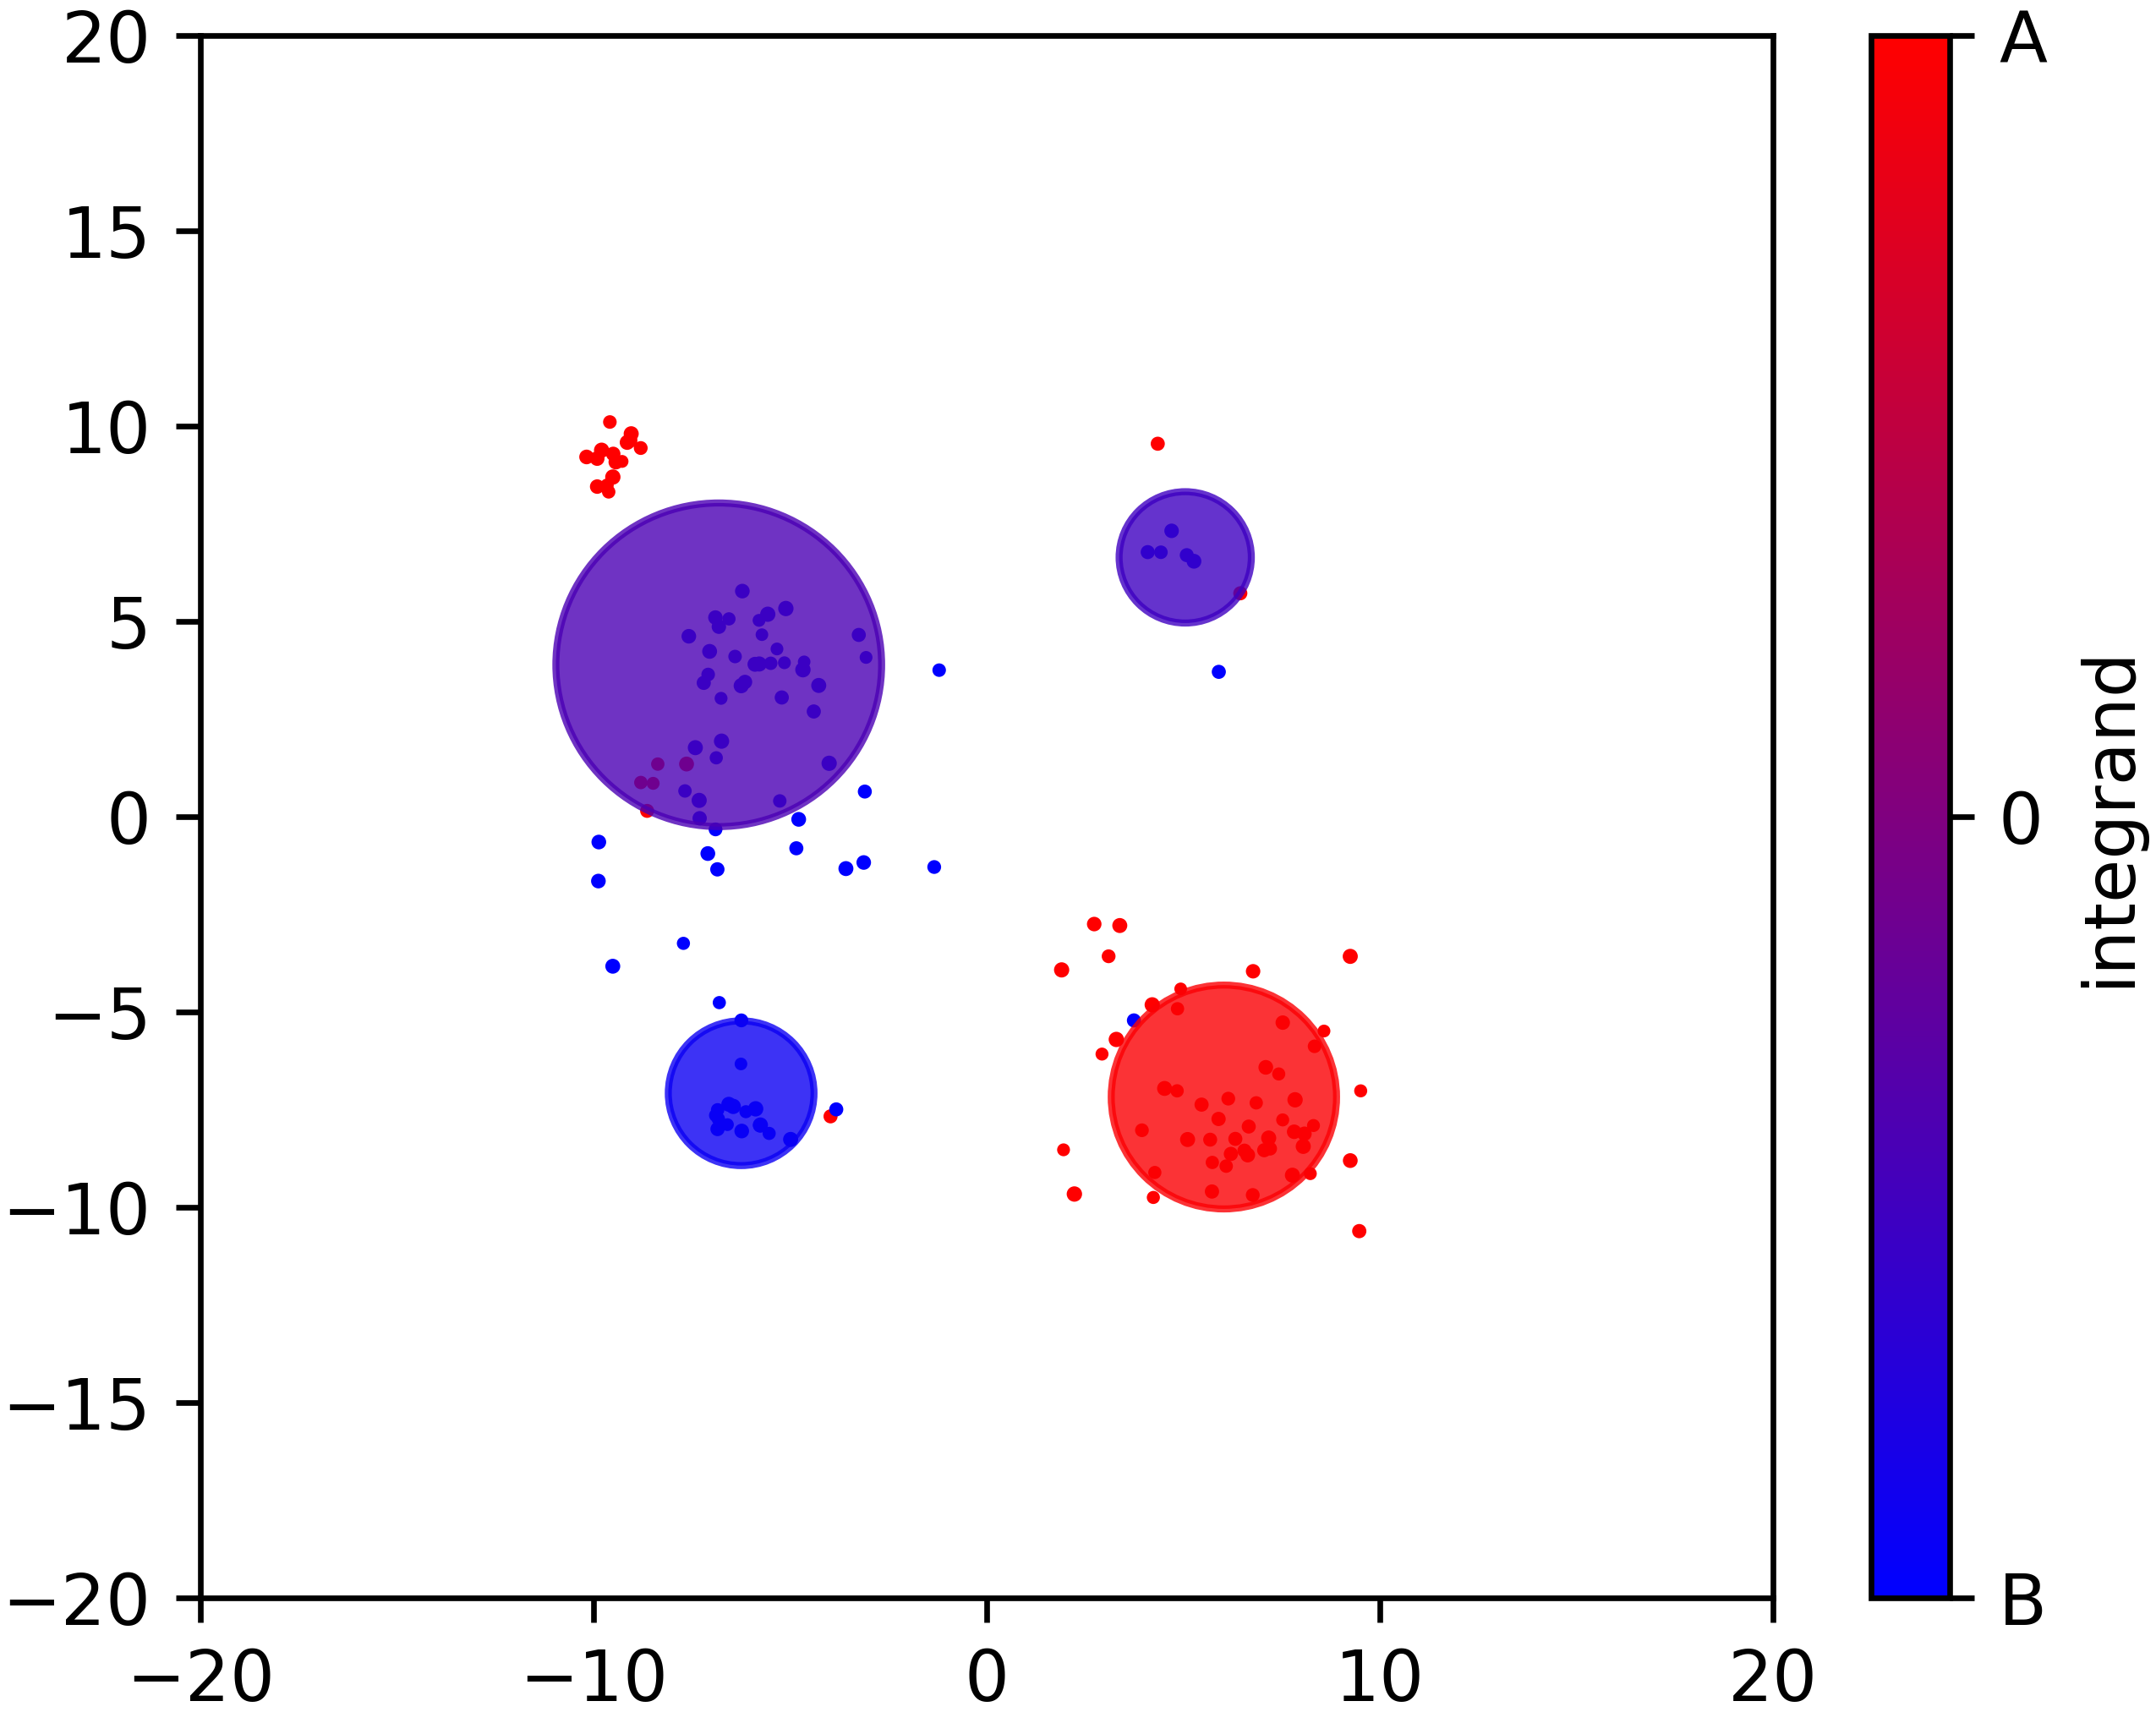
\includegraphics[width=\linewidth]{Figures/kmeans_comparison.png}
		\caption[\gls{kmeans} clustering, example of comparison]{\gls{kmeans} clustering using $4$ centroids.\\ Computed distance: $0.221$.}
		\label{fig:kmeans_clustering}
	\end{subfigure}
	\begin{subfigure}{\linewidth}
		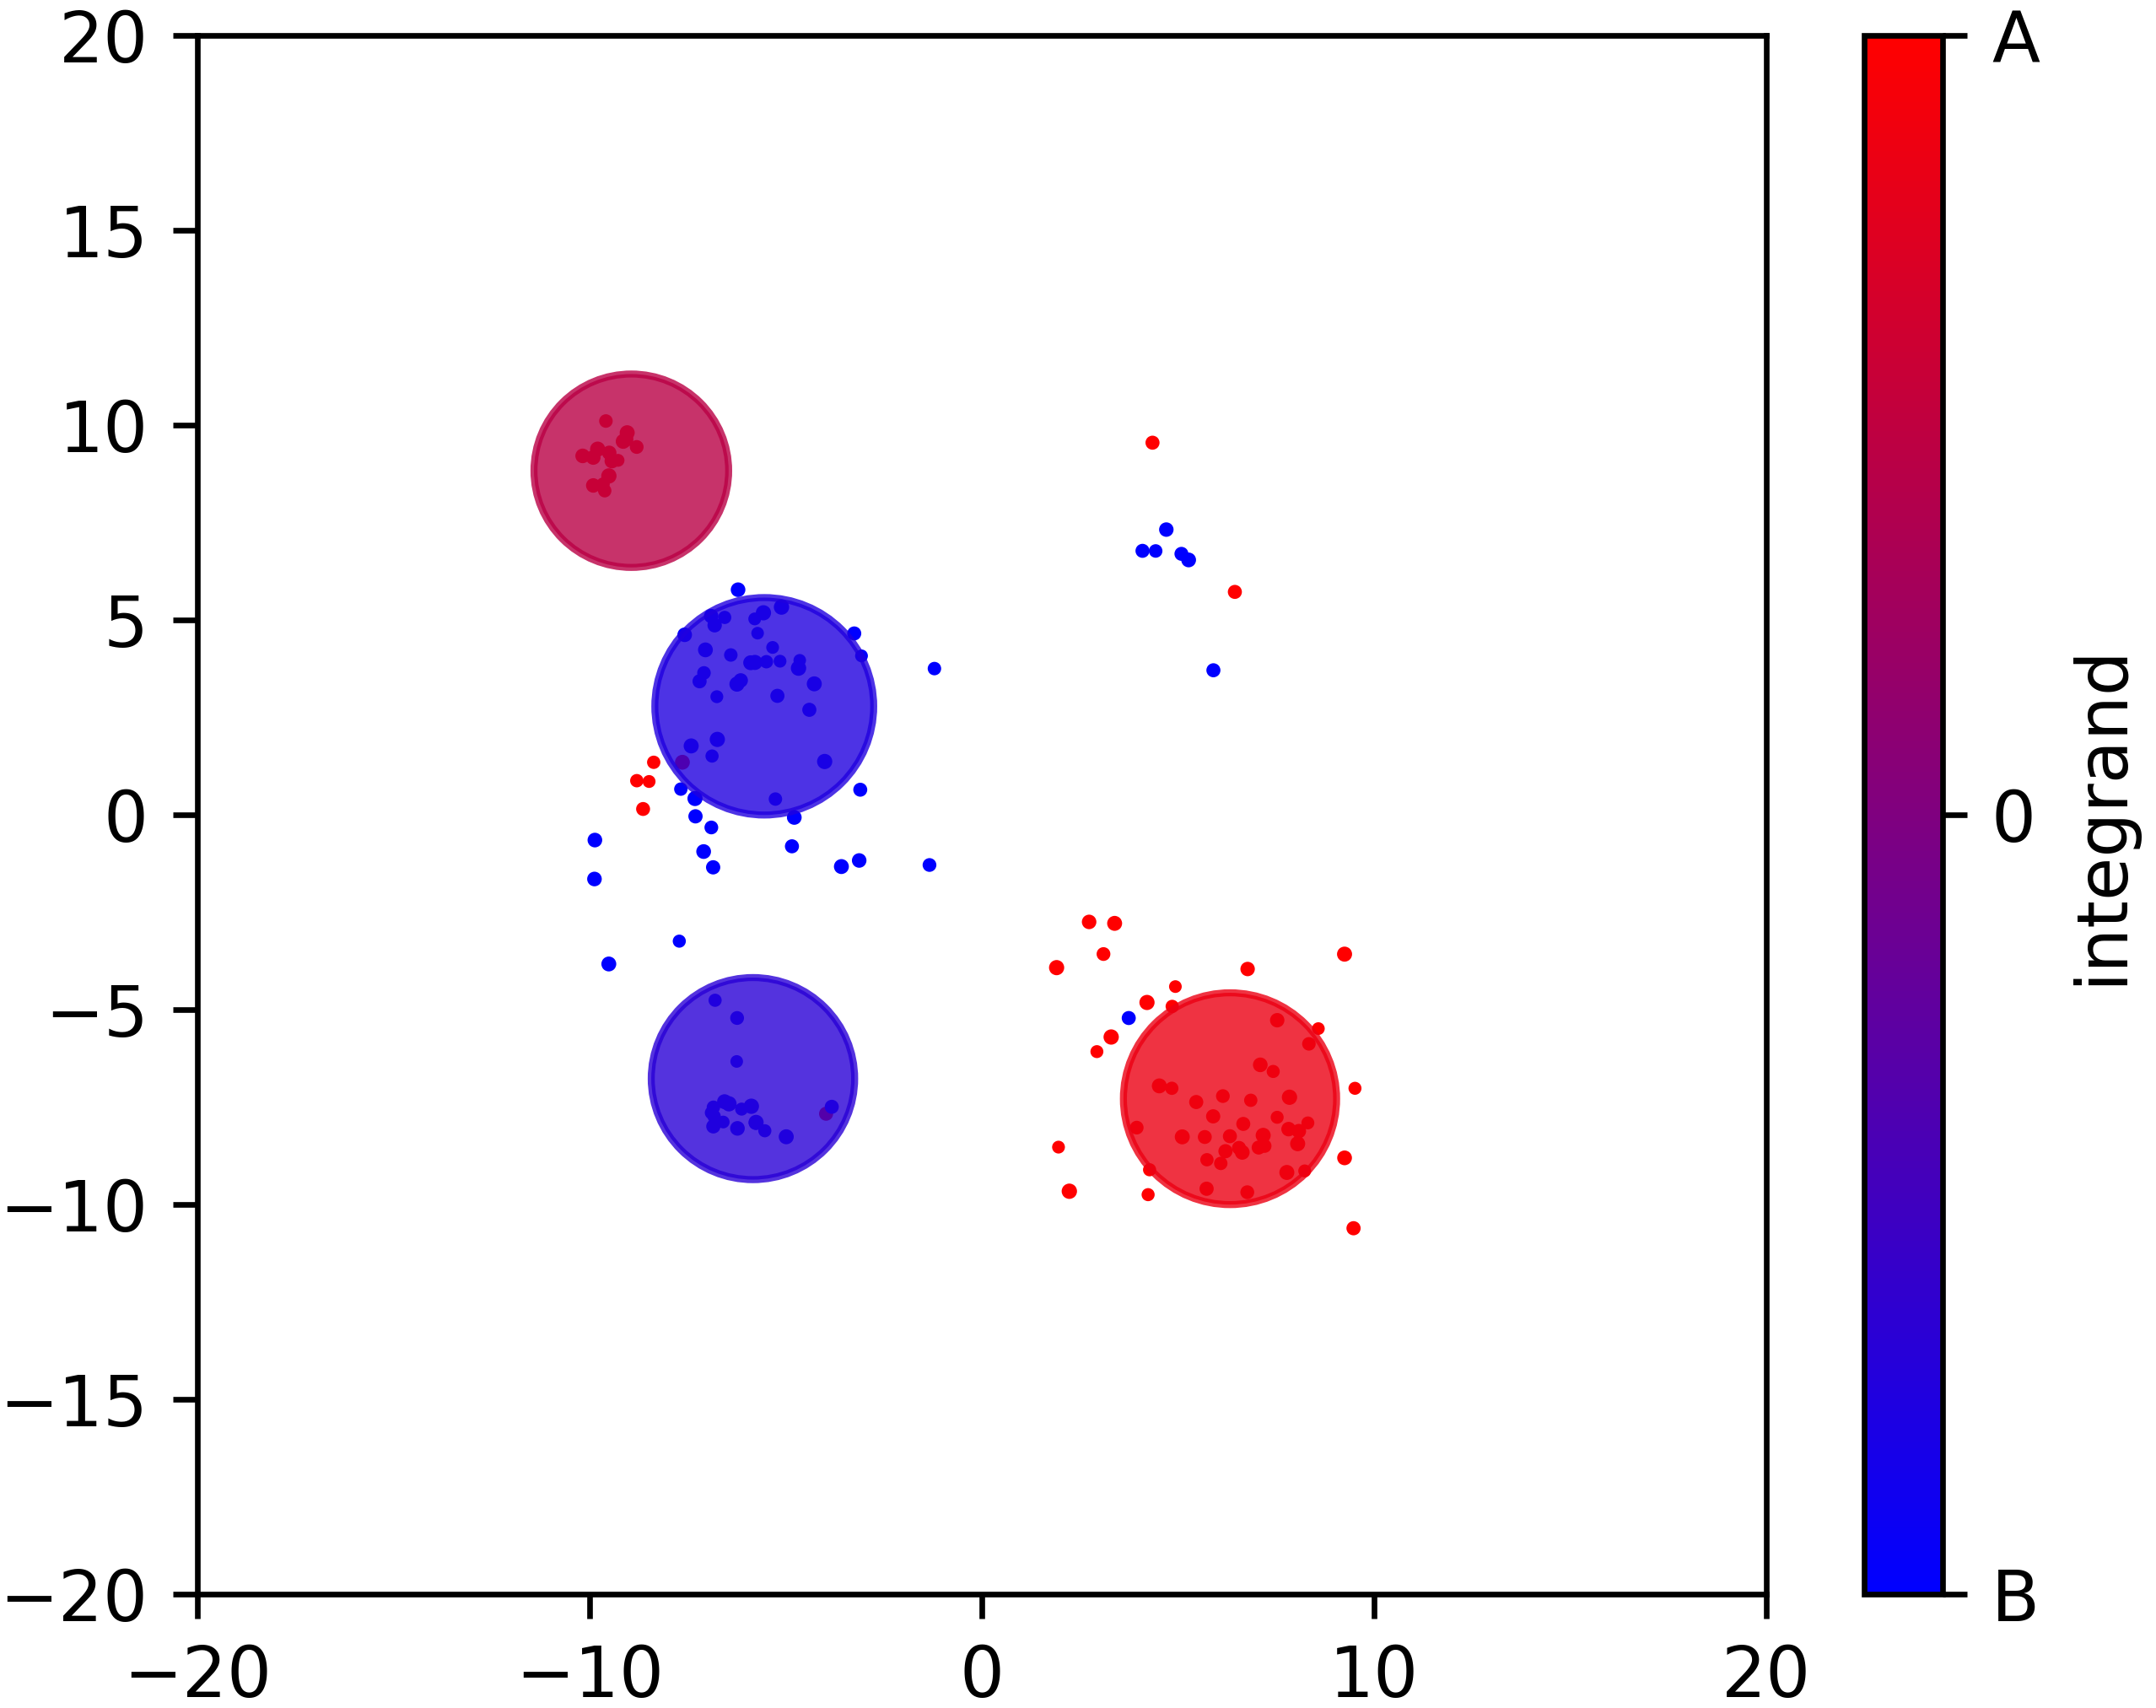
\includegraphics[width=\linewidth]{Figures/fcm_comparison.png}
		\caption[\gls{fcm} clustering, example of comparison]{\gls{fcm} clustering using $4$ centroids.\\ Computed distance $0.289$.}
		\label{fig:fcm_clustering}
	\end{subfigure}
	\caption[example of comparison using $3$ methods]{As can be seen, clusters are assigned a colour that is mapped to $[-1,1]$ ($-1$ is blue, $1$ is red). In particular, this colour is associated with the number $\frac{p_\mathcal{A}(c)-p_\mathcal{B}(c)}{p_\mathcal{A}(c)+p_\mathcal{B}(c)}$ for each cluster of centroid $c$. Furthermore, it is observed that $\gls{kmeans}$ and $\gls{fcm}$ have clusters represented by a circle with area $\mu(c)$ for the two clustering methods.}
\end{figure}
\end{modified}

\begin{modified}
\noindent In order to see the different perspective, we compare the different values obtained from box-clustering, \gls{kmeans} and \gls{fcm}.

\begin{table}[h]
	\centering
	\begin{tabular}{|>{\columncolor{pink}}c|c|c|c|}
		\hline
		\rowcolor{lavender}
		\cellcolor{mint} Values & Box-Clustering & \gls{kmeans} & \gls{fcm} \\
		$\left|D_\mathcal{A}\cap D_\mathcal{B}\right|$ & $4$ & $4$ & $2.889$ \\
		\hline
		$\left|D_\mathcal{A}\cup D_\mathcal{B}\right|$ & $4$ & $4$ & $3.980$ \\
		\hline
		$J_{D_\mathcal{A}, D_\mathcal{B}}$ & $1$ & $1$ & $0.7259$ \\
		\hline
		$\left(1+J_{D_\mathcal{A}, D_\mathcal{B}}\right)^{-1}$ & $0.5$ & $0.5$ & $0.5794$ \\
		\hline
		Integral & $0.5368$ & $0.4418$ & $0.4980$ \\
		\hline
		$d(\mathcal{A},\mathcal{B})$ & $0.268$ & $0.221$ & $0.289$ \\
		\hline
	\end{tabular}
	\caption[Summary of comparison]{Comparing the values obtained from the $3$ algorithms, one can see how \gls{fcm} manages to provide a similar result using fuzzy logic.}
\end{table}
\end{modified}
\begin{toReview}
\begin{exempli_gratia}[Stability of \gls{fcm}]
	Consider a high-dimensional example comparing two sets of samples drawn from two Gaussian distributions with the gradual addition of uniform noise.

	\noindent The goal is to evaluate how noise affects the results obtained from \gls{fcm} compared to \gls{kmeans}.

	\noindent Specifically, we draw two sets of samples from the Gaussian distributions \(\mathcal{N}\left(-\vec{1}, \mathds{1}\right)\) and \(\mathcal{N}\left(\vec{1}, \mathds{1}\right)\) in \(\mathbb{R}^{16}\). Uniform noise with distribution \(\textit{Unif}\left[-5, 5\right]^{16}\) is then added to the data.

	\noindent Each dataset consists of \(500\) samples, combining points from the Gaussian distributions and the noise. The table below shows how the distances between the two distributions decrease as the noise density increases.

	\begin{minipage}{\textwidth}
		\centering
		\begin{tabular}{|>{\columncolor{pink}}c|c|c|}
			\hline
			\rowcolor{lavender}
			\cellcolor{mint} Noise Density & \gls{kmeans} Distance & \gls{fcm} Distance \\
			$0\%$ & $1.000$ & $0.2975$ \\
			\hline
			$1\%$ & $0.5669$ & $0.2427$ \\
			\hline
			$2\%$ & $0.4858$ & $0.2411$ \\
			\hline
			$5\%$ & $0.4076$ & $0.2247$ \\
			\hline
			$10\%$ & $0.0491$ & $0.1921$ \\
			\hline
			$20\%$ & $0.0054$ & $0.1302$ \\
			\hline
		\end{tabular}
	\end{minipage}

	\noindent The results demonstrate that \gls{fcm} is significantly more robust than \gls{kmeans}, as it maintains a discernible distance between the two Gaussian distributions even in the presence of high noise density.
\end{exempli_gratia}
\end{toReview}

\paragraph{\gls{gpu}}
%L'algoritmo presentato è una soluzione sequenziale per l'estrazione delle tessere. Esso lavora iterando attraverso le righe e le colonne dell'immagine, estrae le tessere di dimensioni $N \times N$ e le inserisce in una lista. Tuttavia, questo approccio ha un costo computazionale pari a $O(hwN^2)$.\\
\noindent The \cref{alg:MembershipUpdateSafe} shown is a sequential solution for \gls{fcm}. It works by iterating through the data and centroids to compute the membership matrix. However, this approach has a computational cost of $O(NCk)$.

%Per migliorare l'efficienza computazionale, si può ricorrere all'utilizzo del boost della GPU (General Purpose Graphics Processing Unit). Questo genere di operazioni è noto come GPGPU (General-Purpose computing on Graphics Processing Units). Sfruttare la potenza di calcolo parallelo offerta dalle GPU può notevolmente accelerare il processo di estrazione delle tessere.
\noindent To improve computational efficiency, the use of \gls{gpu} \gls{boost}ing can be employed. This kind of operation is known as \gls{gpgpu}. Exploiting the parallel computing power offered by a \gls{gpu} can greatly accelerate the process of comparison.

%La \gls{gpu}, o unità di elaborazione grafica, è un componente elettronico presente in ogni computer, in grado di eseguire un grande numero di operazioni in parallelo. Originariamente concepita per gestire l'interfaccia grafica nei videogiochi, la \gls{gpu} si trova tipicamente nelle schede grafiche, dove è in grado di visualizzare miliardi di pixel sullo schermo di ogni computer a velocità che la \gls{cpu} non può raggiungere.\\
\noindent The \gls{gpu} is an electronic component present in every computer, able to perform a large number of operations in parallel. Originally designed to handle the graphical interface in video games, the \gls{gpu} is capable of handling billions of pixels on any computer screen at speeds that the \gls{cpu} cannot achieve.

%Questo processore è costituito da migliaia di thread, organizzati gerarchicamente a livello hardware per massimizzarne le prestazioni:
%\begin{enumerate}[label=\roman*.]
%\item \gls{sm}: Esegue un kernel e consiste di numerosi warp;
%\item \gls{warp}: Esegue il kernel del suo stream e possiede una memoria condivisa tra i suoi thread, di solito $32$;
%\item \gls{thread}: Esegue il kernel del suo warp sincronizzandosi con gli altri \gls{thread} dello stesso \gls{warp} e possiede una propria memoria riservata nei suoi registri.
%\end{enumerate}
\noindent This processor is made up of thousands of threads, organised hierarchically at the hardware level to maximise performance:
\begin{enumerate}[label=\roman*.]
\item \gls{sm}: Runs a kernel and consists of numerous \gls{warp}s;
\item \gls{warp}: Runs the kernel of its stream and has shared memory between its threads, usually $32$;
\item \gls{thread}: Executes the kernel of its warp by synchronising with the other \gls{thread}s of the same \gls{warp} and has its own reserved memory in its registers.
\end{enumerate}
%La memoria alla quale può accedere una \gls{gpu} è suddivisa in diverse categorie, tra cui la memoria \textit{global}, \textit{shared}, \textit{cache} e \textit{register}. L'accesso a queste memorie da parte dei \gls{thread} del processore dipende dalla gerarchia dei \gls{thread} stessi. Ad esempio, la memoria \textit{global} è accessibile da ogni \gls{thread}, mentre la memoria \textit{shared} è accessibile solo dai \gls{thread} appartenenti allo stesso \gls{warp}.\\
\noindent The memory that a \gls{gpu} can access is divided into different categories, namely \textit{global}, \textit{shared}, \textit{cache} and \textit{register} memory. Access to these memories by the processor's \gls{thread}s depends on the hierarchy of the \gls{thread}s themselves. For example, the \textit{global} memory is accessible by every \gls{thread}, while the \textit{shared} memory is only accessible by \gls{thread}s in the same \gls{warp}.

%In un computer di alta fascia, è comune trovare schede video dotate di $14$ \gls{sm}, ognuno dei quali contiene $1024$ \gls{thread} suddivisi in $32$ \gls{warp}. Questo totale di $14336$ \gls{thread} può eseguire in parallelo lo stesso identico codice, consentendo un'elaborazione estremamente veloce delle immagini e di altre operazioni che richiedono un alto grado di parallelismo.\\
\noindent In a high-end computer, it is common to find a \gls{gpu} with dozens of \gls{sm}, each containing $64$ or $128$ \gls{core}s. For example, if a process wants to use $\num{1024}$ threads on a single \gls{sm}, the \gls{gpu} will divide these threads into $32$ warps (each containing $32$ threads). Each warp is executed in chunks of $64$ threads at a time, meaning that $2$ warps can be executed simultaneously per clock cycle, while the remaining warps are scheduled for execution in subsequent cycles. This total of tens of thousands of \gls{thread}s can execute the exact same code in parallel, permitting extremely fast processing of images and other operations requiring a high degree of parallelism.

%A partire dagli anni $2000$, l'uso delle \gls{gpu} si è esteso al campo del calcolo scientifico, introducendo importati concetti come la scalabilità e l'\gls{hpc}. Dal $2020$, sono disponibili sul mercato \gls{gpu} dedicate alle operazioni di intelligenza artificiale.\\
\noindent Since the $2000$s, the use of \gls{gpu} has extended to the field of scientific computing, introducing important concepts such as scalability and \gls{hpc}. Since $2020$, dedicated \gls{gpu} are available on the market for artificial intelligence operations.

%In \gls{Python}, esistono framework utili per l'utilizzo delle \gls{gpu}, come \textit{torch} e \textit{TensorFlow}, ampiamente impiegati nell'ambito della computer vision. Tuttavia, anche linguaggi come il \verb"C++" offrono dialetti che consentono di sfruttare queste potenti unità di calcolo. In questo contesto, si userà il dialetto CUDA.\\
\noindent In \gls{Python}, there are useful frameworks for the utilisation of \gls{gpu}, such as \textit{torch} and \textit{TensorFlow}, which are widely employed in the field of computer vision. However, also languages such as \verb "C++" offer dialects that allow these powerful computing units to be exploited. In this paper, the \gls{cuda} dialect will be used.
\footnote{for more details about GPU architecture, see\newline\url{https://researchcomputing.princeton.edu/support/knowledge-base/gpu-computing}}
\footnote{for more details about \gls{cuda} language, see\newline\url{https://docs.nvidia.com/cuda/}}

\bigskip
The integration of \gls{gpgpu} techniques would allow the workload to be distributed over several cores of the \gls{gpu}, thus reducing the time needed for clustering operations. This method is particularly advantageous when handling large amounts of data, as the \gls{gpu} can perform many operations in parallel, speed up computation to be $2000$ times faster than the \gls{cpu} could have done.

\noindent The sum of $N$ numbers can be performed in with computational cost $O(log(N))$. This is because in parallel the \gls{gpu} threads sum one half of the vector over another at the same instant and then repeat until they get a single component that will have only one number. This operation is called \textit{reduction} and we can see it in the \cref{alg:gpu_reduction}. This is just one detail of how the \gls{gpu} can reduce the asymptotic computational cost of an algorithm. Suffice it to say that thanks to reductions and strong parallelism, it is possible to multiply two $N\times K$ and $K\times M$ matrices with cost $O(log(K))$ instead of $O(NMK)$. In clustering many operations can be parallelised and \gls{fcm} in particular requires many sums and linear operations.

\noindent The limitations of \gls{gpu} are not only related to the execution of the same operations on all threads, but also to the nature of these operations. Normally, an instruction takes much longer to be executed by a \gls{gpu} than by a \gls{cpu}. Arithmetic instructions are the most efficient, while the use of conditions tends to be avoided.

\begin{algorithm}
\caption[Parallel algorithm for sum reduction]{Parallel algorithm for sum reduction.\\
	\begin{minipage}[t]{\linewidth}
		\textsc{INPUT}
		\begin{itemize}[noitemsep, topsep=0pt]
			\item[$\textnormal{v}$:] array of values
			\item[$\textnormal{N}$:] number of components
		\end{itemize}
		This algorithm sum all values of an array and write in $\textnormal{v}[0]$ the result. The array is not preserved, in this way the algorithm does not allocate new memory. The computational cost is $O(\log(N))$. In \cref{fig:gpu_reduction} an example over a vector with $7$ components.
	\end{minipage}
}
\begin{algorithmic}[1]
\Procedure{Kernel $\textnormal{i}$, SumReduction}{$\textnormal{v}$,$\textnormal{N}$}
    \State Let $S$ a shared vector with $2^k \geq N$ component
    \State $S[\textnormal{i}] \gets \textnormal{v}[\textnormal{i}]$ if $\textnormal{i}<\textnormal{N}$ else $0$
    \For{$L \gets 2^{k}/2,2^{k}/4,\dots,1$}
        \If{$\textnormal{i} < L$}
            \State $S[\textnormal{i}] \gets S[\textnormal{i}] + S[\textnormal{i}+L]$
        \EndIf
        \State require synchronisation between threads
    \EndFor
\EndProcedure
\label{alg:gpu_reduction}
\end{algorithmic}
\end{algorithm}

\begin{figure}[h]
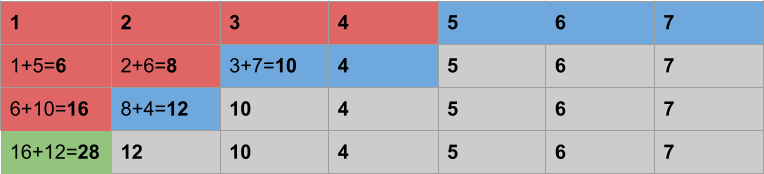
\includegraphics[width=\linewidth]{Figures/example_gpu_reduction.png}
\caption[Application of sum reduction]{We want to calculate the sum of the values in the first row. The idea is to divide the vector into $2$ regions, sum the components, and repeat over the new vector with half the size of the previous vector.}
\label{fig:gpu_reduction}
\end{figure}


% attribution
%\newpage
%\input{main/methodology/Attribution}
  % Corpo vero della tesi in cui si mostra cosa si è fatto
\chapter{Results}
\begin{toDo}
	\section{Architecture}
	Mostrare l'architettura del software a livello implementativo
    \section{Pre processing}
    Mostrare i risultati del pre processing.
    \begin{itemize}
        \item serie di Fourier applicate a griglie sintetiche per dedurre quali sono le frequenze di nostro interesse: griglie dritte e ruotate, griglie chiare e scure, griglie con elementi inquinanti, confronto tra teoria e aspettativa
        \item serie di Fourier applicate a immagini vere, confronto con le immagini sintetiche
        \item mostrare alcuni risultati della pulizia dei quadretti attraverso le varie fasi dell'algoritmo di pulizia
    \end{itemize}
    \section{Synthesis}
    Mostrare una piccola analisi delle sintesi ottenute e della velocità del programma, magari con dettagli implementativi
    \section{Comparison}
   		Mostrare dettagli del clustering a livello esecutivo, come velocità del programma e confronto con l'esecuzione su CPU
    	\subsection{Results}
    		Mostrare dettagli in esecuzione dei vari valori ottenuti dall'algoritmo di comparazione. Quindi concludere con una panoramica dei risultati ottenuti.
\end{toDo}


%\begin{figure}
%	\centering
%	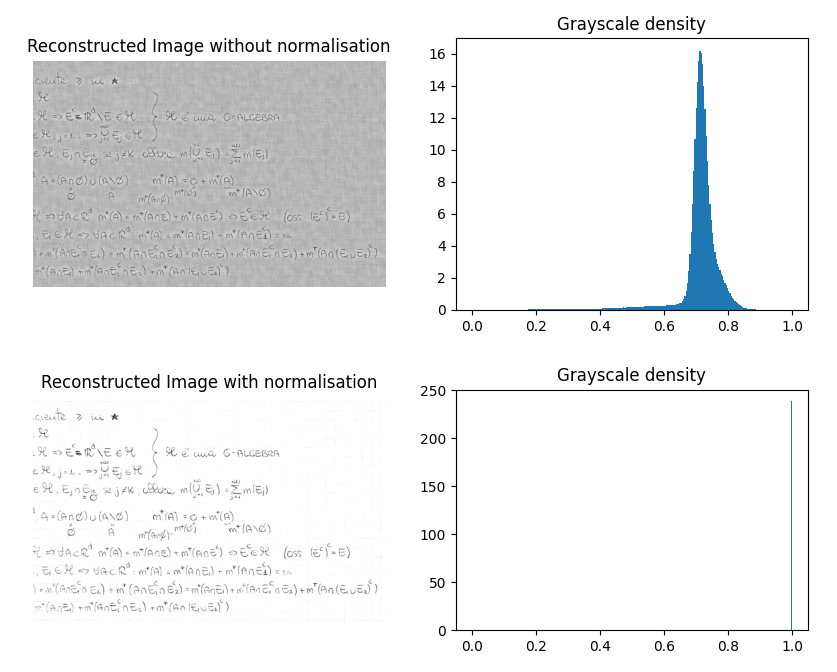
\includegraphics[width=\linewidth]{Figures/first_reconstruct.png}
%	\caption{Come si osserva i grigi si sono molto avvicinati tra loro dopo \gls{fft}, ma è possibile ribilanciare i colori confrontandoli con l'immagine originale.}
%	\label{fig:first_reconstruct}
%\end{figure}
  % Risultati (analisi dei risultati ottenuti in merito la tesi)
%\chapter{Discussion and Conclusions}

\begin{toDo}
	\begin{itemize}
		\item Riassumere i collegamenti tra Results e Methodology
		\item Sottolineare i limiti delle procedure
		\item Proporre varianti da esplorare
	\end{itemize}

\end{toDo}
  % Discussione (confronto tra i risultati e la teoria)
%\chapter{Conclusion}
%Prospettive future, possibili applicazioni.
  % Conclusioni (riepilogo e prospettive future)
\appendix
\chapter{KMeans, GMM, FCM compare figures}

\begin{figure}[h]
	\centering
	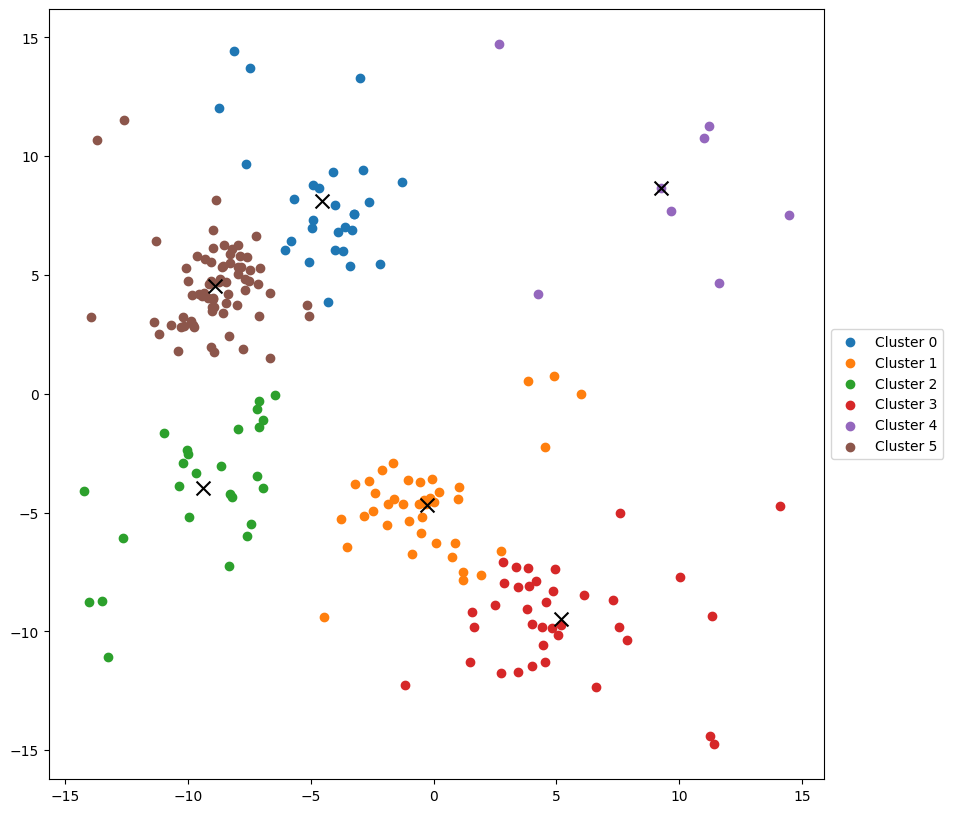
\includegraphics[width=0.9\linewidth]{Figures/dati_kmeans.png}
	\caption[example of \gls{kmeans} clustering]{The data points are coloured according to the calculated label and the estimated centroid is indicated with an $\times$.}
	\label{fig:data_kmeans}
\end{figure}
\begin{modified}
Modificato da \texttt{X} a $\times$
\end{modified}
\begin{figure}[h]
    \centering
    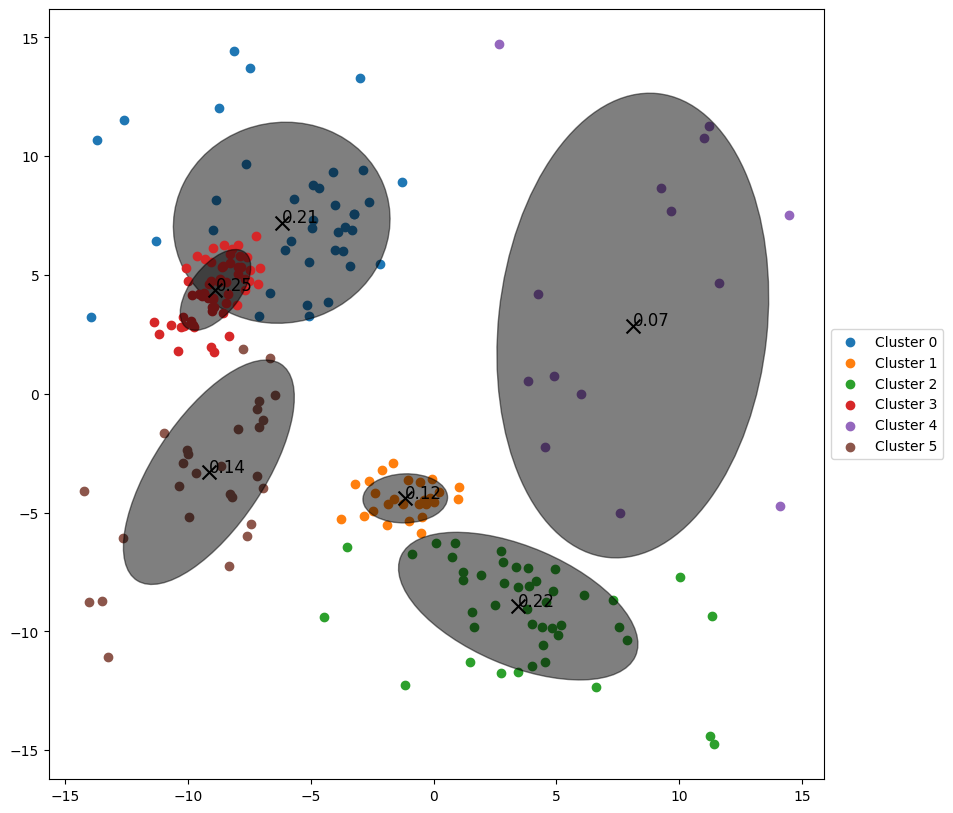
\includegraphics[width=0.9\linewidth]{Figures/dati_gmm.png}
    \caption[example of \gls{gmm} clustering]{The data points are coloured according to the Mahalanobis distance and the estimated centroid is indicated with an $\times$. The ellipse of the normal distribution represents the covariance and is a confidence region of $95\%$.}
    \label{fig:data_gmm}
\end{figure}
\begin{modified}
Modificato da \texttt{X} a $\times$
\end{modified}
\begin{figure}[h]
    \centering
    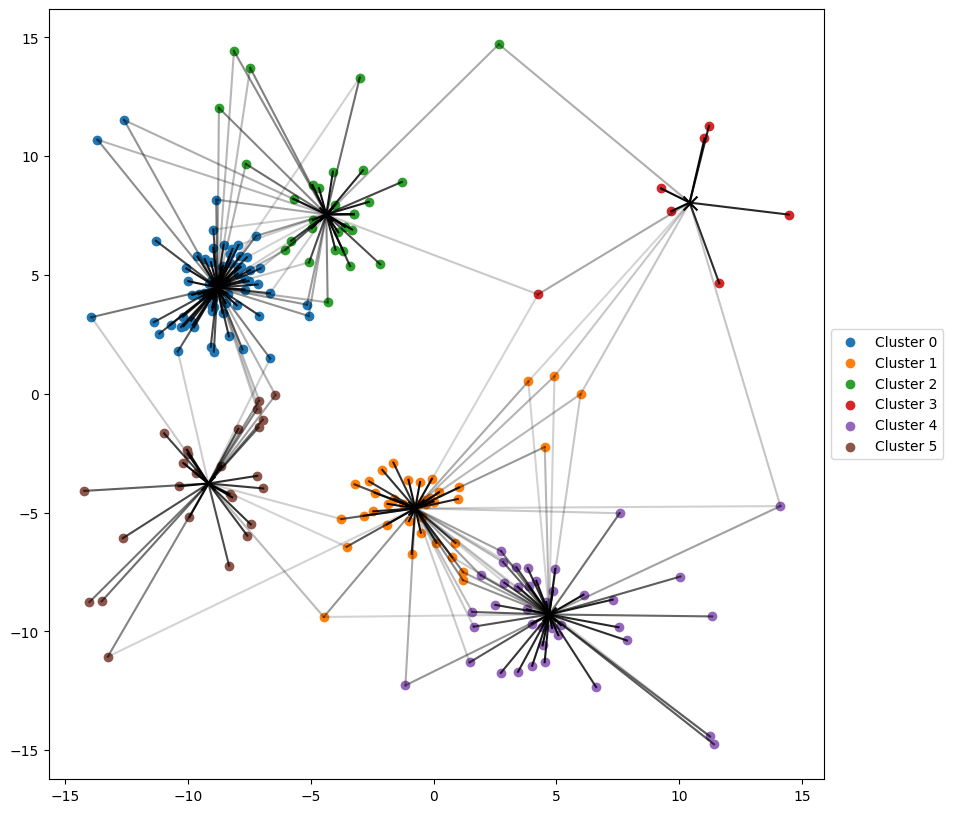
\includegraphics[width=0.9\linewidth]{Figures/dati_fcm.png}
    \caption[example of \gls{fcm} clustering]{The data points are coloured according to the most probable label and the estimated centroid is indicated with an $\times$. The lines indicate the assignments with the greatest degree of affiliation of each point to the clusters; the darker the lines, the stronger the assignment.}
    \label{fig:data_fcm}
\end{figure}
\begin{modified}
Modificato da \texttt{X} a $\times$
\end{modified}

\chapter{FCM implementation with CUDA} \label{appendix:fcm_kernel}
\gls{cuda} è un'architettura hardware supportata dai processori grafici di \emph{NVIDIA}, un'azienda statunitense. E' possibile realizzare il codice che definisce la comunicazione tra \gls{cpu} e \gls{gpu} in un dialetto del \gls{cxx}. Il codice che effettivamente esegue il processore grafico può essere già implementato con funzioni speciali delle librerie \gls{thrust} e \gls{cuBLAS} o realizzato personalmente attraverso dei kernel. In questa appendice si mostra il kernel usato per realizzare il calcolo della matrice $u^2$ in \gls{fcm}. In particolare l'algoritmo è ottimizzato per compiere il calcolo su al più MAX\_THREAD\_PER\_BLOCK centroidi, in questo modo si hanno le maggiori prestazioni poiché si possono usare al meglio le proprietà hardware della \gls{gpu}.

\begin{lstlisting}[style=code, language=C, rulecolor=\color{blue}]
/**
* @brief This kernel computes the matrix U2 of membership between
* data points and centroids
*
* @param[in] d_data : the i-th is d_data[i * n_dimensions + k]
* for k = 0, ..., n_dimensions - 1
* @param[in] d_weights : the weight of the i-th data point is
* d_weights[i]
* @param[in] d_centroids : the j-th is
* d_centroids[j * n_dimensions + k] for k = 0, ..., n_dimensions - 1
* @param[out] d_matrix : the weighted membership between the i-th data point
* and the j-th centroid is stored in d_matrix[i * n_centroids + j]
* @param[out] d_energies : the energy of the i-th data point is stored in
* d_energies[i]
* @param n_data : number of data points
* @param n_dimensions : dimensions of data points
* @param n_centroids : number of centroids
*
* @details This kernel requires a grid of blocks with n_data blocks
* and MAX_THREADS_PER_BLOCK threads for each block.
*
* @note This kernel synchronize threads at the end of the computation
*/
__global__ void
kernel_compute_U2 (const float *const d_data, const float *const d_weights,
const float *const d_centroids, float *const d_matrix,
float *const d_energies, size_t n_data, size_t n_dimensions,
size_t n_centroids)
{
  __shared__ float sdata[MAX_THREADS_PER_BLOCK];
  size_t i = blockIdx.x;  // i-th data
  size_t j = threadIdx.x; // j-th centroid
  float value = 0;
  float reduction_solution = 0;
  float d2 = 0;

  // compute the distance between the i-th data point and the j-th
  // centroid
  if (i < n_data && j < n_centroids)
  {
    for (size_t k = 0; k < n_dimensions; k++)
    {
      float diff = d_data[i * n_dimensions + k]
      - d_centroids[j * n_dimensions + k];
      value += diff * diff;
    }
  }
  d2 = value;
  // syncronyze threads of this block
  __syncthreads ();

  // compute the min value of the block
  if (j < n_centroids)
  sdata[j] = value;
  else
  sdata[j] = FLT_MAX;
  __syncthreads ();
  for (size_t s = MAX_THREADS_PER_BLOCK / 2; s > 0; s >>= 1)
  {
    if (j < s && sdata[j] > sdata[j + s])
    sdata[j] = sdata[j + s];
    __syncthreads ();
  }
  reduction_solution = sdata[0];
  // syncronyze threads of this block
  __syncthreads ();

  // prepare the row to a stable normalization
  if (reduction_solution == 0.0)
  {
    // let to 1 the components that are 0 and to 0 the others
    if (i < n_data && j < n_centroids)
    value = value == 0.0 ? 1.0 : 0.0;
  }
  else
  {
    // for each component of the row, assign min/value
    if (i < n_data && j < n_centroids)
    value = reduction_solution / value;
  }
  // syncronyze threads of this block
  __syncthreads ();

  // compute the sum of the row
  if (j < n_centroids)
    sdata[j] = value;
  else
    sdata[j] = 0.0;
  __syncthreads ();
  for (size_t s = MAX_THREADS_PER_BLOCK / 2; s > 0; s >>= 1)
  {
    if (j < s)
      sdata[j] += sdata[j + s];
    __syncthreads ();
  }
  min_value = sdata[0];
  // syncronyze threads of this block
  __syncthreads ();

  // assign the value to the matrix
  if (i < n_data && j < n_centroids)
  {
    value /= min_value;
    d_matrix[i * n_centroids + j] = value * value * d_weights[i];
  }
  // syncronyze threads of this block
  __syncthreads ();

  // compute energy
  if (i < n_data && j < n_centroids)
    value = d_matrix[i * n_centroids + j] * d2;  // compute partial energy
  // syncronyze threads of this block
  __syncthreads ();

  // compute the sum of the partial energies
  if (j < n_centroids)
    sdata[j] = value;
  else
    sdata[j] = 0.0;
  __syncthreads ();
  for (size_t s = MAX_THREADS_PER_BLOCK / 2; s > 0; s >>= 1)
  {
    if (j < s)
    sdata[j] += sdata[j + s];
    __syncthreads ();
  }
  value = sdata[0];  // energy of the data point
  // syncronyze threads of this block
  __syncthreads ();

  // assign the energy to the matrix
  if (i < n_data && j == 0)
    d_energies[i] = value;
  // syncronyze threads of this block
  __syncthreads ();
}\end{lstlisting}
  % Appendici

\backmatter
\cleardoublepage
\newpage
\printglossary
\phantomsection
\addcontentsline{toc}{chapter}{\glossaryname}
\newpage
\bibliography{bibliography}
\phantomsection
\addcontentsline{toc}{chapter}{\bibname}
\newpage
%\include{Acknowledgments}

\end{document}
